% !TeX program = pdflatex
\documentclass[12pt,a4paper,oneside]{book}


\usepackage{iftex}
\ifXeTeX
  \usepackage{fontspec}
  \usepackage{polyglossia}
  \setdefaultlanguage{english}
  \setotherlanguage{french}
  \setotherlanguage{arabic}
  \makeatletter
  \nofrench@punctuation
  \makeatother
  \setmainfont{TeX Gyre Pagella}
  \setsansfont{TeX Gyre Heros}
  \setmonofont{TeX Gyre Cursor}
  \IfFontExistsTF{Amiri}{%
    \newfontfamily\arabicfont[Script=Arabic,Scale=1.06]{Amiri}%
  }{%
    \IfFontExistsTF{Noto Naskh Arabic}{%
      \newfontfamily\arabicfont[Script=Arabic,Scale=1.06]{Noto Naskh Arabic}%
    }{%
      \newfontfamily\arabicfont[Script=Arabic,Scale=1.06]{Arabic Typesetting}%
    }%
  }%
  \providecommand{\textarabic}[1]{\foreignlanguage{arabic}{#1}}%
\else
  \usepackage[T1]{fontenc}
  \usepackage[utf8]{inputenc}
  \usepackage[french,english]{babel}
  \usepackage{tgpagella}
  \newcommand{\textenglish}[1]{#1}%
  \newcommand{\textarabic}[1]{#1}%
  \newenvironment{Arabic}{}{}%
\fi
\usepackage{geometry}
\usepackage{graphicx}
\usepackage{grffile}
\graphicspath{{Figures/}{Logos/}{images/}{diagrams/}{Screenshots/}}
% svg package removed: Overleaf/pdflatex uses PNG/PDF figures only (no shell-escape)
\usepackage{float}
\usepackage{placeins}
\usepackage{booktabs}
\usepackage{longtable}
\usepackage{tabularx}
\usepackage{array}
\usepackage{amsmath}
\usepackage{amssymb}
\usepackage{setspace}
\usepackage{xcolor}
\usepackage{colortbl}
\definecolor{navyblue}{RGB}{20,55,95}
\usepackage{enumitem}
\usepackage{mdframed}
\PassOptionsToPackage{hyperfootnotes=false}{hyperref}
\usepackage{hyperref}
\usepackage{titlesec}
\usepackage{fancyhdr}
\usepackage{listings}
\usepackage{caption}
\usepackage{microtype}
\usepackage{silence}
\WarningFilter{tracklang}{No `datatool' support for dialect}
\WarningFilter{latex}{Infinite glue shrinkage found in box being split}
\usepackage{afterpage}
\usepackage{pdfpages}
\usepackage[acronym]{glossaries}

\geometry{
    a4paper,
    left=2.5cm,
    right=2.5cm,
    top=2.6cm,
    bottom=2.6cm
}

\setlength{\headheight}{16pt}
\pagestyle{fancy}
\fancyhf{}
\fancyhead[L]{\nouppercase{\leftmark}}
\fancyhead[R]{\thepage}
\renewcommand{\headrulewidth}{0.3pt}
\renewcommand{\footrulewidth}{0pt}

\renewcommand{\chaptermark}[1]{\markboth{\MakeUppercase{#1}}{}}
\renewcommand{\sectionmark}[1]{\markright{\thesection.\ #1}}

\onehalfspacing
\setlength{\parindent}{1.5em}
\setlength{\parskip}{0.12\baselineskip plus 0.04\baselineskip minus 0.04\baselineskip}
\setcounter{secnumdepth}{3}
\setcounter{tocdepth}{3}
\setlength{\emergencystretch}{3em}
\hbadness=10000
\hfuzz=1pt
\setlength{\tabcolsep}{4.5pt}
\setlength{\LTleft}{0pt}
\setlength{\LTright}{0pt}
\setlength{\LTcapwidth}{\textwidth}
\renewcommand{\tabularxcolumn}[1]{>{\raggedright\arraybackslash}m{#1}}

\newcolumntype{Y}{>{\raggedright\arraybackslash}X}
\newcolumntype{P}[1]{>{\raggedright\arraybackslash}p{#1}}

\definecolor{codegreen}{rgb}{0,0.5,0}
\definecolor{codegray}{rgb}{0.45,0.45,0.45}
\definecolor{codepurple}{rgb}{0.58,0,0.82}
\definecolor{backcolour}{rgb}{0.97,0.97,0.95}

\lstdefinestyle{mystyle}{
    backgroundcolor=\color{backcolour},
    commentstyle=\color{codegreen},
    keywordstyle=\color{magenta},
    numberstyle=\tiny\color{codegray},
    stringstyle=\color{codepurple},
    basicstyle=\ttfamily\footnotesize,
    breakatwhitespace=false,
    breaklines=true,
    captionpos=b,
    keepspaces=true,
    numbers=left,
    numbersep=6pt,
    showspaces=false,
    showstringspaces=false,
    showtabs=false,
    tabsize=2
}

\lstset{style=mystyle}
\renewcommand{\lstlistingname}{Code Listing}
\renewcommand{\lstlistlistingname}{List of Code Listings}

\definecolor{primary}{HTML}{1A237E}
\definecolor{accent}{HTML}{0277BD}
\definecolor{success}{HTML}{2E7D32}
\definecolor{warning}{HTML}{BF360C}
\definecolor{lightblue}{HTML}{E3F2FD}
\definecolor{lightgreen}{HTML}{E8F5E9}
\definecolor{lightyellow}{HTML}{FFFDE7}
\definecolor{subtle}{HTML}{546E7A}

\newmdenv[backgroundcolor=lightblue,linecolor=accent,linewidth=1.5pt,
  leftline=true,topline=false,rightline=false,bottomline=false,
  innerleftmargin=10pt,innerrightmargin=8pt,innertopmargin=7pt,innerbottommargin=7pt,
  skipabove=8pt,skipbelow=8pt]{infobox}
\newmdenv[backgroundcolor=lightgreen,linecolor=success,linewidth=1.5pt,
  leftline=true,topline=false,rightline=false,bottomline=false,
  innerleftmargin=10pt,innerrightmargin=8pt,innertopmargin=7pt,innerbottommargin=7pt,
  skipabove=8pt,skipbelow=8pt]{successbox}
\newmdenv[backgroundcolor=lightyellow,linecolor=warning,linewidth=1.2pt,
  leftline=true,topline=false,rightline=false,bottomline=false,
  innerleftmargin=10pt,innerrightmargin=8pt,innertopmargin=7pt,innerbottommargin=7pt,
  skipabove=8pt,skipbelow=8pt]{riskbox}

\newcommand{\reportchapter}[3]{%
  \chapter{#2}%
  \vspace{-0.2cm}
  \begin{center}
    {\small\itshape\color{subtle}#3}
  \end{center}
  \vspace{0.25cm}
}

\newenvironment{dedication}
  {
   \clearpage
   \thispagestyle{empty}
   \vspace*{\stretch{1}}
   \begin{center}
   {\Huge\bfseries Dedication\par}
   \vspace{1cm}
   \itshape
   \begin{minipage}{1\textwidth}
   \raggedright
  }
  {
   \end{minipage}
   \end{center}
   \vspace{\stretch{2}}
   \clearpage
  }
\newcommand\blankpage{%
    \null
    \thispagestyle{empty}%
    \addtocounter{page}{-1}%
    \newpage
}


\hypersetup{
    colorlinks=true,
    linkcolor=black,
    filecolor=black,
    urlcolor=blue,
    pdfauthor={ANOUAR EL IDRISSI},
    pdftitle={Knowledge Graph Exploration and Querying Platform with RAG},
    pdfpagemode=UseOutlines
}

\begin{document}
\hypersetup{pageanchor=false}

\thispagestyle{empty}
\noindent

\includegraphics[height=1.65cm]{Logos/Logo_INPT.png}
\hfill

\includegraphics[height=1.15cm]{Logos/Company_Logo_Scientiae.png}

\vspace{0.45cm}
\begin{center}
{\large \textsc{\textbf{End-of-Study Project Report}}}\\[0.1cm]
{\large \textsc{To obtain the State Engineering Diploma}}\\[0.1cm]
{\large \textsc{\textit{Major: Embedded Systems and Digital Services}}}\\[0.15cm]

\rule{\linewidth}{0.3mm}\\[0.25cm]
{\Large \textbf{Knowledge Graph Exploration}}\\[0.05cm]
{\Large \textbf{and Querying Platform with RAG}}\\[0.12cm]
{\normalsize \textit{Design and implementation of a reasoning multimodal Graph-RAG system}}\\[0.10cm]
\rule{\linewidth}{0.3mm}\\[0.35cm]

{\large \textsc{Project carried out at SCIENTIAE}}\\[0.12cm]
\vspace{0.45cm}

\begin{minipage}{0.9\textwidth}
  \begin{flushleft}\normalsize
    \emph{Authored by:}\\
    Mr. \textsc{ANOUAR EL IDRISSI}
  \end{flushleft}
\end{minipage}\\[0.35cm]

{\normalsize \textit{Defended on Jun 23, 2026 , before the jury composed of:}}\\[0.30cm]

\small
\begin{tabular}{p{1cm}lll}
 & Ms. \textsc{Safae Dahmani} & INPT & - Examiner \\
 & Mr. \textsc{Mouhcine Chami} & INPT & - Examiner \\
 & Ms. \textsc{ASSIA EL HADBI} & INPT & - Internal Supervisor \\
 & Mr. \textsc{Amrouss Issam} & SCIENTIAE & - External Supervisor \\
\end{tabular}
\normalsize

\vspace{0.45cm}

\includegraphics[scale=0.5]{Logos/ZLAFA.png}

\textsc{Institut National des Postes et Télécommunications}\\[0.3cm]
{\normalsize Promotion : 2025/2026}
\end{center}



\afterpage{\blankpage}

\frontmatter

\begin{dedication}
This report is dedicated, first and foremost, to my mother, whose unconditional love, endless sacrifices, and unwavering support have been the foundation of every achievement in my life. Her strength, patience, and encouragement have inspired me throughout my academic journey.

I also dedicate this work to my brother and sisters, whose affection, confidence, and constant encouragement have always motivated me to strive for excellence and persevere through challenges.

To my entire family, thank you for your trust, understanding, and support during every stage of my studies. Your belief in me has been a constant source of strength and determination.

Finally, I dedicate this work to all those who have contributed, directly or indirectly, to my education and personal growth, and who have nurtured my appreciation for scientific rigor, technical discipline, and the pursuit of knowledge.
\end{dedication}

\chapter*{Acknowledgements}
\addcontentsline{toc}{chapter}{Acknowledgements}

I would like to express my sincere gratitude to everyone who contributed to the successful completion of this end-of-study project.

I would first like to thank \textbf{Ms. ASSIA EL HADBI}, my internal supervisor at INPT, for her guidance, rigorous follow-up, and constructive feedback, which helped maintain a demanding academic approach throughout the project.

I also extend my sincere thanks to \textbf{Mr. Amrouss Issam} and \textbf{Mohammed EL AMRANI} for their technical support, availability, and trust during this internship. Their feedback was essential in connecting architectural decisions to the real needs of the platform.

I thank the entire \textbf{Scientiae} team for their welcome, the quality of our exchanges, and the working environment provided during this project. This experience offered a valuable context for deepening key topics in data engineering, natural language processing, and knowledge graphs.

Finally, I thank my teachers and the entire INPT pedagogical staff for the training provided during the engineering program, which supplied the scientific and methodological foundations necessary for completing this report.


\chapter*{Abstract}
\addcontentsline{toc}{chapter}{Abstract}

\begingroup
\setstretch{1.08}

This thesis presents the design and implementation of a reasoning multimodal Graph-RAG platform entitled \textit{Knowledge Graph Exploration and Querying Platform with RAG}. The system combines four complementary capabilities: autonomous web crawling over political sources, dense semantic search over the collected corpus, structured traversal of a Neo4j knowledge graph containing automatically extracted political entities and relations, and grounded answer synthesis supported by the Mistral language model.

The project addresses the limitations of classical retrieval-augmented generation when applied to relational political data. Standard RAG can retrieve relevant passages, but it struggles with multi-hop questions, entity disambiguation, temporal interpretation, and explicit relationship tracking. By integrating vector retrieval with graph-structured evidence, the proposed platform improves the ability to answer complex analytical questions while preserving traceability to source documents.

The implemented architecture includes a three-level crawler, an administrative scheduler, NLP extraction services, deterministic entity resolution, graph persistence, document storage, local vector retrieval, and a user-facing interface for exploration and consultation. The crawler is not limited to a single reference source: it monitors curated RSS feeds, performs query-driven Google News discovery, downloads and parses PDF reports with Docling and PyMuPDF fallback, and exposes operational controls through the administration dashboard. The report also presents the design principles, technical choices, evaluation approach, observed results, and future perspectives of the system.

\noindent\rule[2pt]{\textwidth}{0.5pt}

{\textbf{Keywords:}} Graph-RAG, autonomous crawling, knowledge graph, Neo4j, Mistral, political intelligence, NLP, relation extraction, multi-hop reasoning, distributed systems.

\noindent\rule[2pt]{\textwidth}{0.5pt}
\endgroup


\chapter*{Résumé}
\addcontentsline{toc}{chapter}{Résumé}

\begingroup
\setstretch{1.08}

\begin{otherlanguage}{french}
Ce rapport présente le projet de fin d'études réalisé au sein de la société \textbf{Scientiae} et portant sur la conception et la mise en œuvre d'une plateforme \textit{Graph-RAG} multimodale pour l'exploration et l'interrogation d'un graphe de connaissances avec génération de réponses fondées. Le système combine quatre capacités complémentaires~: un crawl web autonome sur des sources politiques, une recherche sémantique dense sur le corpus collecté, un parcours structuré d'un graphe de connaissances \textbf{Neo4j} contenant des entités et relations politiques extraites automatiquement, et une synthèse de réponses appuyée sur les preuves à l'aide du modèle \textbf{Mistral}. L'objectif est de transformer l'information politique non structurée en une couche de connaissance traçable, exploitable et analysable.

Le projet répond aux limites de la génération augmentée par récupération classique lorsqu'elle est appliquée à des données politiques relationnelles. Le RAG standard peut retrouver des passages pertinents, mais il peine sur les questions multi-sauts, la désambiguïsation d'entités, l'interprétation temporelle et le suivi explicite des relations. En intégrant la récupération vectorielle à des preuves structurées sous forme de graphe, la plateforme proposée améliore la capacité à répondre à des questions analytiques complexes tout en préservant la traçabilité vers les documents sources.

L'architecture retenue sépare la collecte des données, l'orchestration asynchrone, le traitement du langage naturel et les stockages intermédiaires, avant la publication dans \textbf{Neo4j} et l'indexation des segments dans \textbf{ZVec}. La chaîne de collecte couvre la surveillance de flux \textbf{RSS} sélectionnés, la découverte d'actualités via \textbf{Google News}, le téléchargement et l'analyse de rapports \textbf{PDF}, ainsi qu'un tableau de bord d'administration pour la planification et la supervision. La chaîne de traitement comprend le nettoyage, l'extraction d'entités et de relations, la résolution déterministe des référents, le stockage documentaire dans \textbf{MongoDB}, puis l'interrogation via une interface \textbf{React} avec plusieurs modes de raisonnement (\texttt{rag}, \texttt{cot}, \texttt{reflexive}) et un enrichissement possible par recherche web en direct.

La plateforme a été évaluée sur un banc de quatorze questions classées (factuelles, relationnelles, temporelles, comparatives) à l'aide de métriques de type \textbf{RAGAS}, après optimisation des prompts. Les résultats montrent une progression nette du mode \textbf{RAG} vers le mode réflexif, tandis que le rappel du contexte demeure le principal levier d'amélioration. Le graphe de connaissances et la plateforme qui l'entoure constituent une couche réutilisable pour l'aide à la décision, l'analyse politique et l'exploitation structurée de l'information.
\end{otherlanguage}

\noindent\rule[2pt]{\textwidth}{0.5pt}

\begin{otherlanguage}{french}
{\textbf{Mots-clés~:}} Graph-RAG, graphe de connaissances, Neo4j, Mistral, crawl autonome, intelligence politique, traitement du langage naturel, extraction de relations, génération augmentée par récupération, systèmes distribués.
\end{otherlanguage}

\noindent\rule[2pt]{\textwidth}{0.5pt}
\endgroup


% ------------------------------------------------------------------
% Arabic abstract disabled for pdfLaTeX compilation.
% Arabic Unicode text and right-to-left typesetting require XeLaTeX.
%
% To enable the Arabic abstract:
% 1. Change the compiler to XeLaTeX.
% 2. Uncomment the following line:
%
% \chapter*{\textarabic{ملخص}}
\addcontentsline{toc}{chapter}{arabic Abstract}

\begingroup
\setstretch{1.12}

\begin{otherlanguage}{arabic}
يقدم هذا التقرير مشروع نهاية الدراسة المنجز داخل شركة \textenglish{\textbf{Scientiae}} والمتعلق بتصميم وتنفيذ منصة \textenglish{\textit{Graph-RAG}} متعددة الوسائط لاستكشاف الرسم البياني المعرفي والاستعلام عنه مع توليد إجابات موثقة. يجمع النظام بين الزحف الذاتي على المصادر السياسية، والبحث الدلالي الكثيف فوق المجموعة النصية المجمعة، والاجتياز المنظم لرسم بياني معرفي في \textenglish{\textbf{Neo4j}} يضم كيانات وعلاقات سياسية مستخرجة آليا، وتوليف إجابات مؤسسة على الأدلة بمساعدة نموذج \textenglish{\textbf{Mistral}}. يهدف المشروع إلى تحويل المعلومات السياسية غير المهيكلة إلى طبقة معرفية قابلة للتتبع والاستكشاف والتحليل.

يعالج المشروع محدوديات الجيل المعزز بالاسترجاع الكلاسيكي عند تطبيقه على المعطيات السياسية ذات البعد العلائقي. يمكن للاسترجاع التقليدي إيجاد مقاطع ذات صلة، لكنه يواجه صعوبة في الأسئلة متعددة القفزات، وإزالة لبس الكيانات، والتفسير الزمني، وتتبع العلاقات بشكل صريح. ومن خلال دمج الاسترجاع الشعاعي مع أدلة منظمة على شكل رسم بياني، تحسن المنصة المقترحة القدرة على الإجابة عن أسئلة تحليلية معقدة مع الحفاظ على إمكانية الرجوع إلى الوثائق المصدرية.

تعتمد المنصة على معمارية تفصل بين جمع المعطيات، والأوركسترا غير المتزامنة، ومعالجة اللغة الطبيعية، والتخزين الوسيط، ثم النشر في \textenglish{\textbf{Neo4j}} وفهرسة المقاطع في \textenglish{\textbf{ZVec}}. وتشمل سلسلة الجمع مراقبة تدفقات \textenglish{\textbf{RSS}} المنتقاة، واكتشاف الأخبار عبر \textenglish{Google News}، وتنزيل وتفكيك تقارير \textenglish{PDF}، مع لوحة إدارة للجدولة والإشراف. وتشمل سلسلة المعالجة التنظيف، واستخراج الكيانات والعلاقات، وحل الإحالات المرجعية بشكل حتمي، وتخزين الوثائق في \textenglish{\textbf{MongoDB}}، ثم تمكين الاستعلام عبر واجهة \textenglish{\textbf{React}} بأنماط تفكير متعددة (\textenglish{rag}، \textenglish{cot}، \textenglish{reflexive}) مع إمكانية تعزيز الاسترجاع ببحث ويب مباشر.

أجري تقييم المنصة على مجموعة من أربعة عشر سؤالا مصنفة (واقعي، علائقي، زمني، مقارن) بمقاييس من نوع \textenglish{\textbf{RAGAS}} بعد تحسين الموجهات. وأظهرت النتائج تحسنا تدريجيا من نمط \textenglish{RAG} إلى نمط التفكير الانعكاسي، مع بقاء استدعاء السياق محورا للتحسين المستقبلي. ويُنظر إلى الرسم البياني المعرفي والمنصة المحيطة به بوصفهما طبقة معرفية قابلة لإعادة الاستعمال في الاستشارة والتحليل السياسي والاستغلال المنظم للمعلومة.
\end{otherlanguage}

\noindent\rule[2pt]{\textwidth}{0.5pt}

\begin{otherlanguage}{arabic}
{\textbf{الكلمات المفتاحية:}} \textenglish{Graph-RAG}، رسم بياني معرفي، \textenglish{Neo4j}، \textenglish{Mistral}، زحف ذاتي، استخبارات سياسية، معالجة اللغة الطبيعية، استخراج العلاقات، استرجاع معزز بالتوليد، أنظمة موزعة.
\end{otherlanguage}

\noindent\rule[2pt]{\textwidth}{0.5pt}
\endgroup

% ------------------------------------------------------------------

\listoffigures
\addcontentsline{toc}{chapter}{List of Figures}

\listoftables
\addcontentsline{toc}{chapter}{List of Tables}


\chapter*{List of Acronyms}
\addcontentsline{toc}{chapter}{List of Acronyms}

\renewcommand{\arraystretch}{1.2}

\begin{longtable}{p{3cm} p{11cm}}
\toprule
\textbf{Acronym} & \textbf{Meaning} \\
\midrule
\endhead

ANN    & Approximate Nearest Neighbour \\
AI     & Artificial Intelligence \\
API    & Application Programming Interface \\
BLEU   & Bilingual Evaluation Understudy \\
CoT    & Chain of Thought \\
CSS    & Cascading Style Sheets \\
CRUD   & Create, Read, Update, Delete \\
CSV    & Comma-Separated Values \\
DFD    & Data Flow Diagram \\
DPR    & Dense Passage Retrieval \\
DSPy   & Declarative Self-improving Python \\
ERD    & Entity Relationship Diagram \\
FR     & Functional Requirements \\
F1     & Harmonic Mean of Precision and Recall \\
GDELT  & Global Database of Events, Language, and Tone \\
GKG    & Global Knowledge Graph \\
GPU    & Graphics Processing Unit \\
GQA    & Grouped-Query Attention \\
GraphQL & Graph Query Language \\
HTML   & HyperText Markup Language \\
HTTP   & HyperText Transfer Protocol \\
JSON   & JavaScript Object Notation \\
JWT    & JSON Web Token \\
KG     & Knowledge Graph \\
LLM    & Large Language Model \\
MIPRO  & Multi-prompt Instruction Proposal Optimizer \\
MRR    & Mean Reciprocal Rank \\
MS     & Microsoft \\
NFR    & Non-Functional Requirement \\
NER    & Named Entity Recognition \\
NLP    & Natural Language Processing \\
OCR    & Optical Character Recognition \\
PDF    & Portable Document Format \\
QA     & Question Answering \\
RAG    & Retrieval-Augmented Generation \\
RAGAS  & Retrieval-Augmented Generation Assessment \\
RDF    & Resource Description Framework \\
REST   & Representational State Transfer \\
ROUGE  & Recall-Oriented Understudy for Gisting Evaluation \\
RSS    & Really Simple Syndication \\
SAS    & Semantic Answer Similarity \\
SLI    & Service Level Indicator \\
SOA    & Service-Oriented Architecture \\
SPARQL & SPARQL Protocol and RDF Query Language \\
SQL    & Structured Query Language \\
SSE    & Server-Sent Events \\
TKG    & Temporal Knowledge Graph \\
UI     & User Interface \\
URI    & Uniform Resource Identifier \\
URL    & Uniform Resource Locator \\
UX     & User Experience \\
XML    & eXtensible Markup Language \\
YAML   & YAML Ain't Markup Language \\

\bottomrule
\end{longtable}




\tableofcontents
\addcontentsline{toc}{chapter}{Table of Contents}

\hypersetup{pageanchor=true}
\mainmatter

% General Introduction
\chapter*{General Introduction}
\addcontentsline{toc}{chapter}{General Introduction}

The digital transformation of political communication has produced an unprecedented volume of public information. News agencies, parliamentary bodies, governmental institutions, research organizations, and civil society actors publish large numbers of articles, reports, and official documents every day. These sources contain valuable signals about actors, events, institutions, alliances, conflicts, financial links, and temporal changes, but most of this information remains embedded in unstructured text.

For analysts, journalists, and researchers, the difficulty is no longer only to access information, but to connect dispersed facts and interpret them in a reliable way. Keyword search can retrieve documents, and classical retrieval-augmented generation can summarize passages, yet both approaches remain limited when the question requires entity disambiguation, multi-hop reasoning, temporal filtering, and explicit source attribution.

This difficulty is amplified by the rhythm of political information. Relevant evidence may appear first in an RSS entry, then in a full news article, then in an institutional report or policy PDF. A platform designed for political intelligence must therefore do more than consume a static dataset. It must continuously discover, collect, normalize, and evaluate heterogeneous sources while preserving the provenance of every fact. In this project, that role is fulfilled by an autonomous crawler composed of several complementary levels: curated RSS monitoring, query-driven news discovery, PDF report ingestion, and administrative controls for scheduled collection.

Within its research and development activities, SCIENTIAE is developing a
sovereign Graph-RAG framework designed to adapt to different domains rather
than remain tied to a single use case. The framework provides reusable
components for data acquisition, LLM-based knowledge extraction, graph
construction, semantic retrieval, evidence-grounded answer generation, and
system evaluation. A new domain can therefore be integrated by adapting its
sources, entity and relation models, extraction rules, and evaluation
questions while preserving the same core architecture.

Politics and geopolitics were selected as the application and validation domain for this work because they provide a demanding environment for testing the framework. Political intelligence analysis often depends on relational questions: a user may need to understand how two actors are connected, which events created a diplomatic shift, how an institution evolved over time, or which documents support a specific claim. Such questions cannot be answered robustly by treating documents as isolated text fragments; they require a representation that combines textual evidence with structured relations.

The implemented system constitutes a domain-specific instance of this broader
multimodal Graph-RAG framework. It combines dense semantic retrieval, a Neo4j
knowledge graph, DSPy-optimized entity and relation extraction during
ingestion, and an LLM-based reasoning layer. Its goal is to transform a large
corpus of political and geopolitical information into an exploitable
knowledge layer that supports grounded, explainable, and temporally aware
analysis. The resulting platform serves both as a functional decision-support
tool and as an experimental environment for assessing how the framework can
later be adapted to other domains.

A second challenge concerns data acquisition itself. Many Graph-RAG systems assume that the corpus already exists and focus only on retrieval and generation. In this project, the corpus is produced by the platform. The crawler must avoid duplicates, preserve source metadata, handle heterogeneous formats, operate politely with external websites, and provide enough operational visibility for an administrator to supervise ingestion. This makes crawling and ingestion a central contribution of the project rather than a peripheral utility.

The final challenge is trust. Political analysis is sensitive because a generated answer may influence the interpretation of institutions, actors, or conflicts. The system must therefore expose its evidence, separate raw documents from extracted relations, preserve timestamps, and make retrieval behavior auditable. This need explains the combination of MongoDB for document storage, Neo4j for explicit relations, ZVec for local semantic search, and observability tools for operational monitoring.

To address these challenges, the project pursues three main objectives. The
first is to contribute to a modular Graph-RAG framework whose principal
processing stages can be configured for different domains. The second is to
instantiate this framework for political and geopolitical analysis by
implementing an autonomous ingestion and knowledge-graph construction
pipeline together with a reasoning engine that combines vector retrieval,
graph traversal, and cited answer synthesis. The third is to evaluate the
system in terms of extraction reliability, retrieval quality, answer
grounding, reasoning depth, and response time.

These objectives are translated into concrete engineering goals. The platform must collect data autonomously from RSS feeds, Google News queries, direct URLs, and PDF sources. It must normalize the collected material into document records that can be processed by the same extraction pipeline. It must resolve entities deterministically through canonical names and stable identifiers, without depending on a Wikidata backbone as the main source of truth. It must also provide an administration interface where ingestion status, scheduler state, logs, source filters, and backfill operations can be controlled without modifying code.

From a user perspective, the objective is to provide an integrated analytical workspace. The analyst can ask questions in natural language, inspect sources, explore graph neighborhoods, follow political trends, consult documents, and observe system health. From an engineering perspective, the objective is to build a modular pipeline in which crawling, extraction, graph publication, chunking, embedding, retrieval, and evaluation remain separable and testable.

The expected contribution is therefore both methodological and practical. Methodologically, the project studies how autonomous crawling, knowledge graph construction, and retrieval-augmented generation can be combined in a reusable, domain-adaptable workflow. Practically, it delivers and evaluates a political and geopolitical implementation in which source acquisition, evidence structuring, semantic search, graph exploration, and answer generation are connected through operational backend services and frontend controls.

The remainder of this report is organized into five chapters. Chapter~1
introduces the host organization, project context, problem statement,
objectives, actors, requirements, technology choices, and project-management
approach. Chapter~2 presents the state of the art concerning knowledge graphs,
retrieval-augmented generation, Graph-RAG, ingestion strategies, embeddings,
and large language models. Chapter~3 describes the system architecture, data
flows, domain model, ingestion pipeline, and reasoning design. Chapter~4
details the implementation, persistence layers, interfaces, deployment,
observability, and optimization mechanisms. Finally, Chapter~5 presents the
system evaluation and performance analysis, including RAGAS metrics,
reasoning-mode comparison, embedding performance, DSPy-based knowledge
extraction optimization, requirements validation, and limitations.


% Chapter 1 -- structure from table of content.md; writing style from README_STYLE_PFE.md

\reportchapter{1}{Context and State of the Art}{Institutional context, project motivation, theoretical foundations, and research positioning.}

\section{Introduction}

In this chapter, the end-of-study internship is situated within the research environment of the host organization, SCIENTIAE, and the theoretical background required to understand the platform developed during the PFE is reviewed. The chapter first presents the company and the constraints of political intelligence analysis, then surveys large language models, retrieval-augmented generation, knowledge graphs, political NLP, and reasoning paradigms. It closes by stating the research gap and the positioning of the project. This progression moves from institutional context to scientific foundations before Chapter~2 formalizes requirements, actors, and validation criteria.

\section{Host Organization Overview}

\subsection{Company Profile}

This graduation project took place at \textbf{SCIENTIAE}, the host organization in Rabat. Before the technical chapters, it is useful to recall the institutional setting in which the platform was designed, tested, and progressively enriched with real political data.

\begin{figure}[H]
    \centering
    \vspace{1cm}
    
\includegraphics[height=1.5cm]{Logos/Company_Logo_Scientiae.png}
    \caption{SCIENTIAE, host organization of the end-of-study internship.}
    \label{fig:host-organization}
    \vspace{1cm}
\end{figure}

SCIENTIAE is an emerging company based in Hay Riad, Rabat, oriented towards high-tech activities in data, security, and digital solutions. Its offering is centered on consulting, support, and tailored solution design, with a commitment to service quality, industry standards, and innovation.

Beyond this profile, SCIENTIAE provides a favorable environment for exploratory engineering work in software engineering, data processing, automation, and knowledge valuation. This context offered technical autonomy and a clear application domain for a platform devoted to extracting, enriching, and structuring knowledge from heterogeneous textual sources. The PFE therefore fits the company's R\&D strategy aimed at sovereign decision-intelligence solutions for institutional partners.

\subsection{Organizational Structure}

The internal organization of SCIENTIAE is summarized below to clarify how the project was supervised and integrated. The company is structured around a General Management from which two major poles are deployed: an Administrative Department (Human Resources, Finance) and a Research and Development Department coordinating software engineering, data science engineering, and cybersecurity engineering.

\begin{figure}[H]
    \centering
    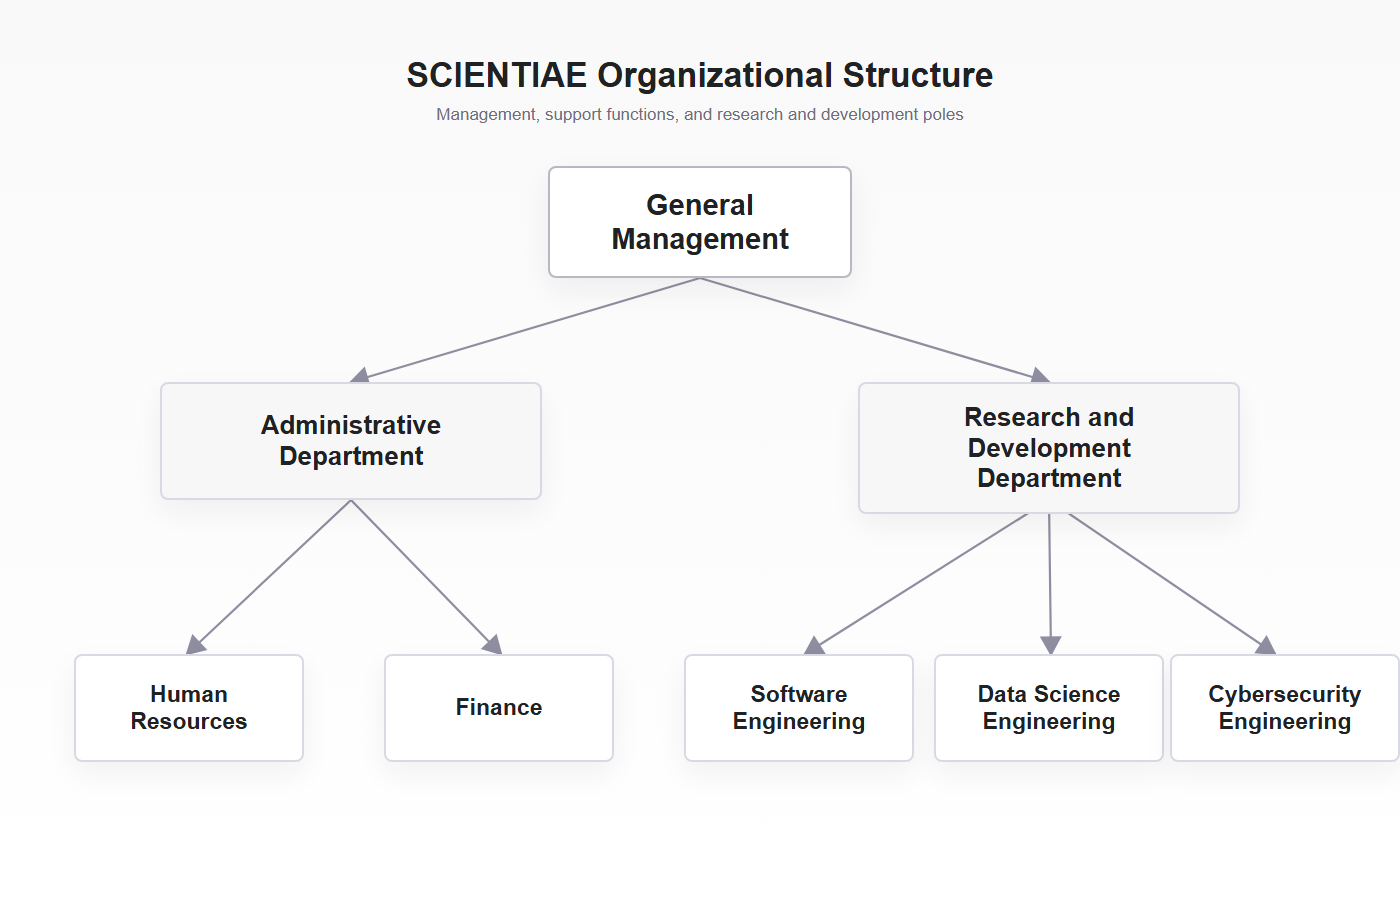
\includegraphics[width=0.96\textwidth,height=0.78\textheight,keepaspectratio]{images/org_chart.png}
    \caption{Organizational structure of SCIENTIAE.}
    \label{fig:org-chart}
\end{figure}

Figure~\ref{fig:org-chart} summarizes this organization. The project was anchored in the R\&D pole, which facilitated regular exchanges with profiles specialized in data and platform development. The internship was conducted under academic supervision at INPT and professional supervision at SCIENTIAE, with periodic reviews of progress, architecture choices, and demonstration milestones. The technical stack, component boundaries, and deployment choices are detailed in Chapters~3 and~4 rather than in this contextual section.

\subsection{Services and R\&D Focus}

The R\&D pole combines three complementary professions that shaped the orientation of the project. Cybersecurity supports the protection of information systems and incident monitoring. Web development covers application services, hosting, and user interfaces. Data science, the most central orientation here, focuses on structuring and exploiting large volumes of data to extract actionable knowledge. A knowledge-graph approach follows this logic: political documents are transformed into structured evidence that can be queried, explored, and reasoned over.

From a technological perspective, the internship mobilized a modern data-and-AI stack rather than a monolithic toolchain. Figure~\ref{fig:tech-overview} illustrates representative components: Python and FastAPI for backend services, React for the analytical interface, DSPy for structured LLM orchestration \cite{khattab-dspy}, and containerized deployment for reproducibility. The platform also relies on document, graph, vector, and cache stores, together with observability tooling. These families are introduced here only as context; versions, APIs, schemas, and engineering trade-offs are presented in the design and implementation chapters.

\begin{figure}[H]
    \centering
    \raisebox{-0.15\height}{
\includegraphics[height=0.95cm]{Logos/python.png}}\hspace{0.6cm}
    \raisebox{-0.15\height}{
\includegraphics[height=0.95cm]{Logos/fastapi.png}}\hspace{0.6cm}
    \raisebox{-0.15\height}{
\includegraphics[height=0.95cm]{Logos/react.png}}\hspace{0.6cm}
    \raisebox{-0.15\height}{
\includegraphics[height=0.95cm]{Logos/dspy_logo.png}}
    \caption{Representative technologies of the R\&D environment (detailed architecture in Chapters~3--4).}
    \label{fig:tech-overview}
\end{figure}

This overview clarifies why the PFE could be conducted as applied research with industrial constraints rather than as a purely theoretical study. The following section addresses the political intelligence context that motivated the platform.

\section{Project Context and Motivation}

\subsection{Political Intelligence Challenges}
\label{sec:political-intelligence-challenges}

Political intelligence targets a domain where information is abundant but difficult to exploit reliably. Analysis requires connecting actors, institutions, events, alliances, and temporal changes that are rarely stated explicitly in a single document. Keyword search and classical retrieval-augmented generation remain weak when the question depends on entity disambiguation, multi-hop relations, or temporal consistency.

Three recurring limitations motivate a hybrid architecture. First, flat retrieval cannot navigate explicit relationships between actors. Second, surface forms such as ``The President'' and ``Macron'' may be treated as distinct entities without resolution. Third, standard RAG often treats retrieved chunks as equally current, which leads to temporal drift when political positions evolve. These constraints are developed further in the state of the art and translated into requirements in Chapter~2.

\subsection{Data Volume and Heterogeneity}

Before any reasoning layer can operate, a political intelligence platform must obtain a reliable and continuously updated corpus. Web crawling is therefore a foundational requirement rather than a peripheral utility. Unlike large-scale search engines, the objective is constrained: prioritize relevant sources, preserve provenance, avoid duplicates, and produce clean documents for downstream NLP extraction.

The target platform must support complementary collection strategies: curated monitoring of RSS feeds and official portals; query-driven discovery through news aggregators; and document-oriented ingestion of PDF reports. Operational supervision (scheduling, manual triggers, logs) is also required so that freshness does not compromise control. Unlike approaches centered on a fixed external knowledge base, the PFE aims at a system that builds its own corpus and then extracts graph knowledge from collected evidence. The engineering realization of these ingestion levels is described in Chapter~4.

\subsection{Need for Evidence Traceability}

Autonomous crawling introduces a quality challenge that differs from classical information retrieval. A crawler decides what enters the corpus, which affects extraction quality, graph reliability, retrieval precision, and answer faithfulness. Traceability therefore requires preserving source URL, source name, topic, publication date, scraping date, language, and quality indicators, together with deduplication to limit syndication bias.

Another principle is to separate acquisition from interpretation: collection should remain broad, while extraction and graph publication decide whether a document contains political entities, relations, or events worth keeping. Table~\ref{tab:crawler-positioning} compares the \emph{design target} of the platform with common acquisition approaches. In the table, ``real-time updates'' for curated RSS means scheduled refresh of known feeds, not unconstrained open-web recrawl.

\begin{table}[H]
\centering
\scriptsize
\renewcommand{\arraystretch}{1.25}
\begin{tabularx}{\textwidth}{@{}>{\bfseries\raggedright\arraybackslash}p{3.1cm}XXXX@{}}
\toprule
\rowcolor{lightblue}
Approach & Source Coverage & Format Handling & Freshness & Operational Control \\
\midrule
Manual collection & Limited to analyst effort & Depends on user work & Irregular & No automation \\
Simple RSS reader & Curated feeds only & RSS summaries and linked articles & Scheduled feed refresh & Limited monitoring \\
One-shot web scraper & Targeted pages & Usually HTML only & Poor after execution & Weak supervision \\
External knowledge base & Structured reference data & Already normalized & Not focused on breaking news & Dependent on external updates \\
\textbf{Platform design target} & RSS, news discovery, direct URLs, PDF sources & HTML, RSS, PDF, normalized records & Scheduled and triggerable collection & Supervised dashboard and logs \\
\bottomrule
\end{tabularx}
\caption{Positioning of the platform ingestion design against common acquisition approaches.}
\label{tab:crawler-positioning}
\end{table}

The table highlights a deliberate choice: political intelligence depends on freshness, provenance, format diversity, and supervision rather than on a single channel. Manual collection and simple RSS readers lack operational depth; one-shot scrapers degrade over time; external knowledge bases are strong on structure but weak on breaking news under local control. The platform design target combines broader coverage with supervisable ingestion, at the cost of higher engineering complexity. Having established this context, the following section reviews the scientific foundations that informed the architectural choices retained for the platform.

\section{State of the Art}

\subsection{Large Language Models}

Large language models (LLMs) are neural sequence models based on the Transformer architecture \cite{vaswani-attention}. Self-attention computes, for each token, a weighted combination of all other token representations, which enables long-context modeling and parallel training at scale. This mechanism underpins contemporary extraction, classification, and answer synthesis pipelines.

Several model families are discussed in the literature and in industrial practice. Proprietary models such as GPT-4 offer strong reasoning but raise privacy and data-sovereignty concerns for sensitive political analysis. Open-weight families such as LLaMA~3 reduce vendor lock-in but may require substantial local GPU resources at scale. European foundation models such as Mistral Large are often selected when regulatory alignment and API governance matter. Independently of the vendor, LLMs remain subject to hallucination and to knowledge cutoffs unless generation is grounded in external retrieval \cite{lewis-rag}.

For the PFE, these observations justify an architecture where the LLM is not the sole source of truth. Parametric knowledge is complemented by retrieved documents, graph facts, and explicit citations, as developed in the following subsections.

\subsection{Retrieval-Augmented Generation (RAG)}

Retrieval-Augmented Generation (RAG) augments LLM generation with dynamically retrieved external knowledge \cite{lewis-rag}. The classical pipeline indexes documents by chunking and embedding them, retrieves the top-$k$ relevant passages for a query, and conditions answer generation on that evidence. This workflow is efficient for direct factual questions but structurally limited for relational political analysis, as noted in Section~\ref{sec:political-intelligence-challenges}.

Recent extensions focus on \textbf{evidence grounding and citation}: retrieved passages are linked to sources, incomplete evidence triggers additional retrieval, and confidence checks reduce unsupported synthesis. These mechanisms do not replace RAG; they make generation auditable, which is essential when answers may influence interpretation of institutions, actors, or conflicts. Grounding also prepares the transition to graph-backed retrieval, where evidence includes explicit relations rather than isolated text spans.

\subsection{Knowledge Graphs and Graph-RAG}

Classical RAG retrieves passages through semantic similarity. Graph-RAG constructs graph-structured knowledge from a corpus and retrieves through entities, relationships, communities, and source passages \cite{edge-graphrag,microsoft-graphrag}. Figure~\ref{fig:rag-vs-graphrag} contrasts the two retrieval paths and shows why geopolitical questions often require relational traversal.

\begin{figure}[H]
    \centering
    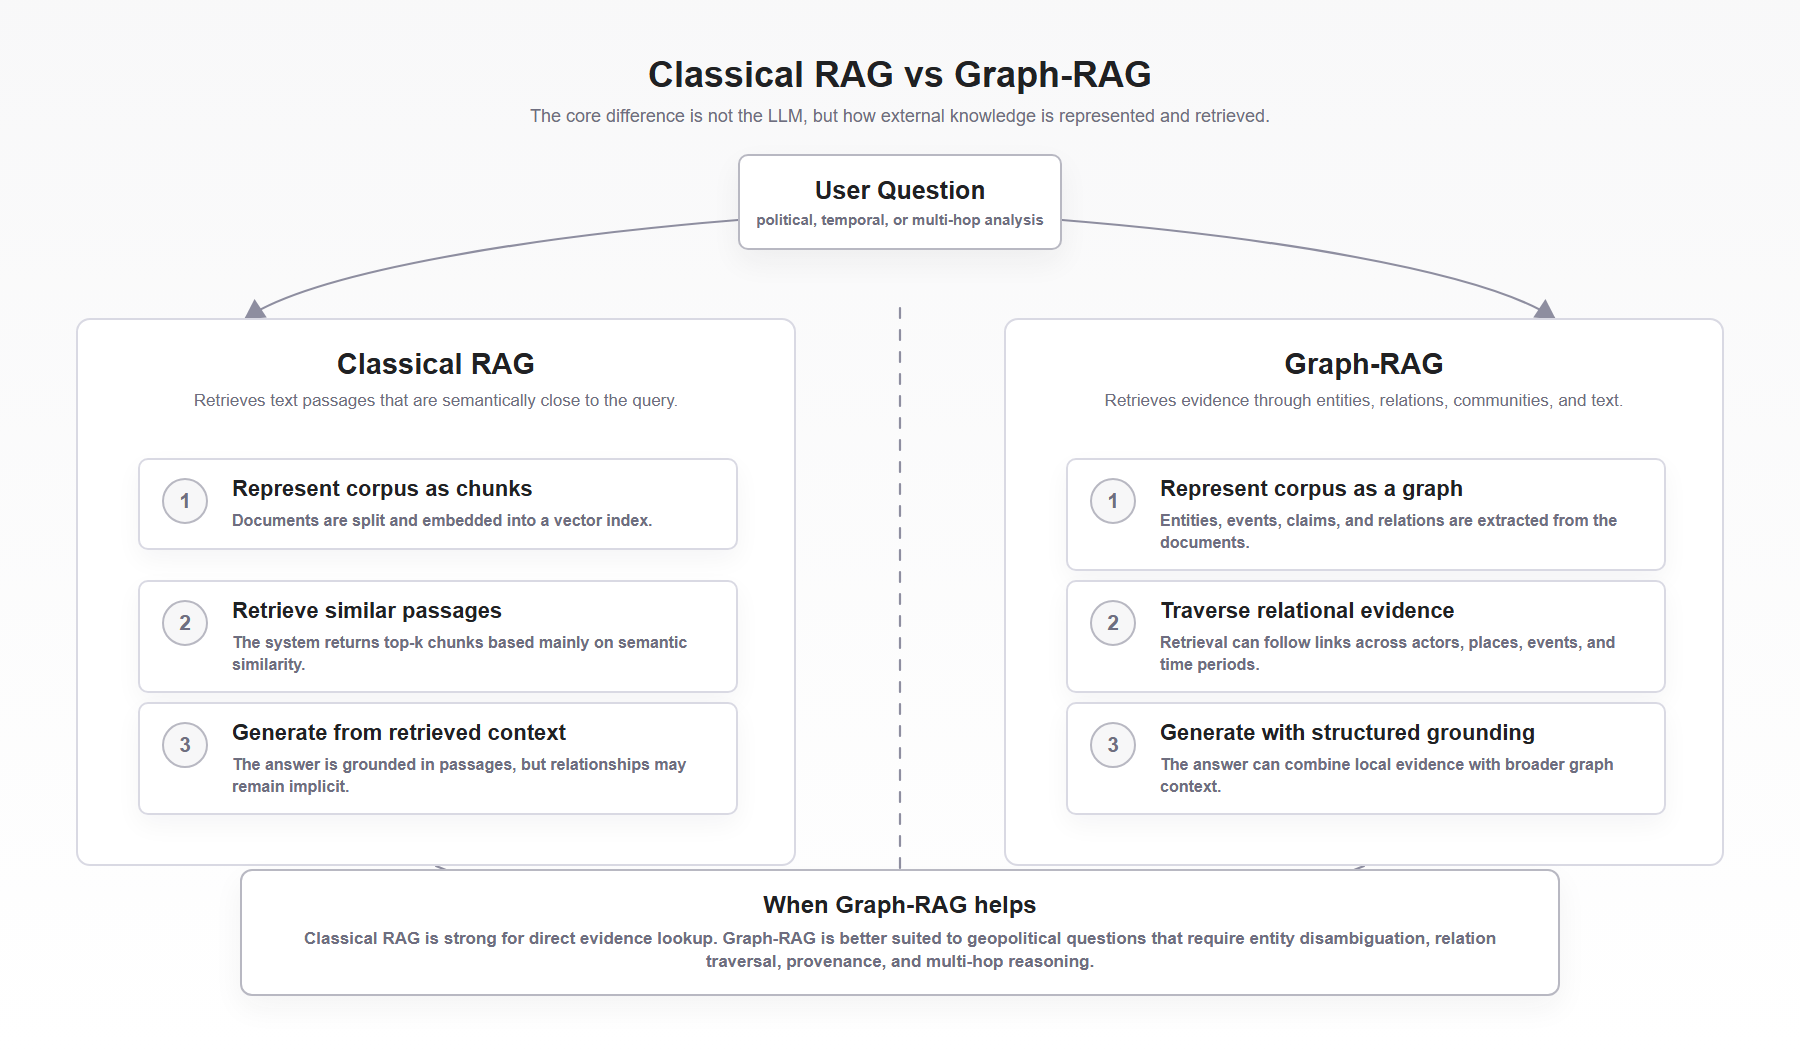
\includegraphics[width=0.96\textwidth,height=0.78\textheight,keepaspectratio]{images/rag_vs_graphrag.png}
    \caption{Comparison between classical RAG and Graph-RAG retrieval paths.}
    \label{fig:rag-vs-graphrag}
\end{figure}

\textbf{Knowledge graph concepts.} A knowledge graph represents entities and typed relations, optionally with temporal or provenance metadata. It supports entity disambiguation, path queries, and hybrid retrieval that combines vector similarity with structural constraints.

\textbf{Graph construction from text.} Pipelines typically perform extraction, entity resolution, and provenance linking so that each relation remains traceable to a source document. Noise control is critical because LLM-based extraction can introduce spurious nodes or edges if resolution rules are weak.

\textbf{Graph-RAG retrieval and reasoning.} Once published, the graph enables multi-hop traversal, community summarization, and fusion with textual chunks retrieved by dense search \cite{edge-graphrag,microsoft-graphrag}. This combination is particularly relevant when answers depend on chains of actors and events rather than on a single paragraph.

\subsection{LLM Reasoning and Thinking Modes}

Beyond retrieval format, recent work studies how a language model \emph{uses} evidence during generation. Classical RAG follows a mostly linear pipeline: retrieve once, then generate. This design is efficient for localized factual questions, but it is structurally weak when a query requires several retrieval steps, intermediate planning, or verification of partial evidence \cite{lewis-rag}.

\textbf{Chain-of-Thought and query decomposition.} Chain-of-Thought (CoT) prompting asks the model to produce intermediate reasoning steps before the final answer \cite{wei-cot}. In retrieval settings, decomposition splits a complex question into sub-questions and guides evidence collection step by step. The goal is not longer answers for their own sake, but better coverage when the first retrieved batch is incomplete.

\textbf{Interleaved retrieval and multi-hop reasoning.} IRCoT interleaves retrieval with ongoing chain-of-thought generation: each reasoning step can trigger a new retrieval call guided by what was learned in the previous step \cite{trivedi-ircot}. This pattern is especially relevant for multi-hop questions where bridge entities only become visible after an initial pass. When knowledge is graph-structured, multi-hop traversal plays a similar role by following explicit paths between actors and events rather than relying on lexical similarity alone.

\textbf{ReAct and tool-interleaved control.} ReAct combines reasoning traces with actions such as search, graph lookup, or tool invocation \cite{yao-react}. Instead of a fixed retrieve-then-generate sequence, the model alternates between thinking steps and operations on external memory. This architecture is a precursor to modern agentic pipelines in which a controller decides when to retrieve again, when to stop, and when to synthesize.

\textbf{Reflection and Self-RAG.} Reflection-based methods add a critique step that evaluates whether the current evidence supports the draft answer. Self-RAG trains the model to decide when retrieval is needed, when generation is sufficient, and when the output should be revised \cite{asai-selfrag}. These approaches reduce unsupported synthesis at the cost of additional model calls and higher latency.

\textbf{Agentic RAG.} Agentic RAG generalizes the above patterns into loops that may include planning, routing, iterative retrieval, critique, and final synthesis. Surveys of the field describe a recurring trade-off: iterative and reflective pipelines improve faithfulness on relational or multi-step tasks, but they increase token cost and response time compared with naive RAG. For political intelligence, this literature motivates architectures in which reasoning depth can be adapted to question complexity rather than forcing every query through the heaviest pipeline.

Chapter~4 presents the reasoning modes implemented in the platform and describes how these ideas are operationalized in production.

\subsection{Political NLP and Temporal Modeling}

Political NLP extends language understanding to actors, institutions, stances, conflicts, and temporal relations. \textbf{Entity and relation extraction} increasingly relies on joint models that predict tuples under schema constraints, reducing error propagation compared with rigid pipelines. \textbf{Stance and conflict analysis} aims to detect how an actor relates to a target event or entity; zero-shot and weakly supervised methods are common when labeled political data are scarce \cite{allaway-stance}. \textbf{Temporal knowledge graphs} attach validity intervals to facts so that snapshot and trend queries remain consistent when information evolves \cite{trivedi-hyte}.

Together, these strands explain why political intelligence systems combine NLP extraction, temporal modeling, and retrieval architectures rather than a single summarization model.

\subsection{Related Systems and Gap Analysis}

Table~\ref{tab:comparative-summary} compares representative families of approaches along criteria relevant to political intelligence. The comparison is intentionally literature-oriented: it does not claim that one row is universally superior, but it reveals structural trade-offs that motivate the platform studied in this PFE.

\begin{table}[H]
\centering
\scriptsize
\renewcommand{\arraystretch}{1.25}
\begin{tabularx}{\textwidth}{@{}>{\bfseries\raggedright\arraybackslash}X >{\centering\arraybackslash}p{1.42cm} >{\centering\arraybackslash}p{1.42cm} >{\centering\arraybackslash}p{1.42cm} >{\centering\arraybackslash}p{1.42cm} >{\centering\arraybackslash}p{1.42cm} >{\centering\arraybackslash}p{1.42cm}@{}}
\toprule
\rowcolor{lightblue}
Approach & Multi-hop reasoning & Entity disambiguation & Temporal reasoning & Source citation & Structured queries & Scheduled corpus refresh \\
\midrule
Classical RAG & No & No & No & Yes & No & Yes \\
MS GraphRAG & Yes & Yes & Partial & Yes & No & No \\
Knowledge Graph & Yes & Yes & Yes & Partial & Yes & Yes \\
\bottomrule
\end{tabularx}
\caption{Comparative summary of major approach families (literature-oriented criteria).}
\label{tab:comparative-summary}
\end{table}

Classical RAG supports citation and scheduled refresh of indexed corpora but lacks explicit multi-hop and temporal modeling. Microsoft GraphRAG improves structured retrieval but is not designed as a continuously supervised political ingestion platform. Pure knowledge graphs excel at structured and temporal queries but do not, by themselves, provide conversational synthesis with the same interaction model as a chat-oriented RAG interface. No single row satisfies all criteria; the remaining challenge is to integrate ingestion, hybrid retrieval, graph reasoning, and grounded generation in one auditable workflow.

\section{Research Gap and Positioning}
\label{sec:research-gap-positioning}

The central research gap is the inability of classical retrieval systems to represent political information as evolving relational structures. Semantic search can surface topically similar documents, but it does not explicitly model who is connected to whom, through which event, under which institutional role, and during which temporal interval.

The platform developed during the internship addresses this gap through a hybrid architecture. Dense vector retrieval contributes semantic recall over unstructured documents, while the knowledge graph contributes relational precision, entity disambiguation, and multi-hop traversal. Compared with Table~\ref{tab:comparative-summary}, the contribution of this PFE does not claim universal superiority on every criterion; rather, it targets an integrated combination that was missing in the compared families:

\begin{itemize}[leftmargin=*, itemsep=4pt]
\item \textbf{Hybrid evidence:} joint use of vector chunks, graph relations, and document provenance in the same query workflow.
\item \textbf{Supervised ingestion:} autonomous collection with operational control, rather than a static benchmark corpus only.
\item \textbf{Selectable reasoning depth:} one-hop, decomposed multi-hop, and reflexive modes to trade latency against analytical coverage (Chapter~4).
\item \textbf{Remaining limits:} semantic deduplication, full temporal normalization, and large-scale multilingual coverage are still partial and are discussed in Chapter~5.
\end{itemize}

From this perspective, the project contributes along three axes:

\begin{itemize}[leftmargin=*, itemsep=4pt]
\item \textbf{Methodological contribution:} studying how graph-structured evidence improves faithfulness, explainability, and temporal consistency of LLM-based political analysis.
\item \textbf{Technical contribution:} combining ingestion, hybrid retrieval, graph publication, and reasoning modes in one platform grounded in provenance.
\item \textbf{Operational contribution:} delivering an end-to-end workflow in which analysts query evidence, inspect sources, explore graph neighborhoods, and supervise ingestion without modifying backend code.
\end{itemize}

In functional terms, the system is a reasoning multimodal Graph-RAG platform: it collects heterogeneous political documents, converts them into chunks and graph relations, retrieves evidence through vector and graph stores, and produces cited answers through an LLM orchestration layer (Mistral with DSPy modules, as detailed in Chapter~4). This gap therefore corresponds to a concrete need observed during the internship: analysts require continuous ingestion, structured knowledge, semantic retrieval, and explainable generation in a single environment.

\section{Conclusion}

This chapter situated the PFE within SCIENTIAE and the domain of political intelligence. It explained why traceable ingestion and hybrid evidence matter, reviewed the state of the art on LLMs, RAG, Graph-RAG, reasoning paradigms, and political NLP, and stated the research gap addressed by the platform. Methodologically, the project studies graph-structured grounding; technically, it integrates ingestion, hybrid retrieval, and selectable reasoning; operationally, it provides a supervised analyst workflow. Chapter~2 will now formalize requirements, actors, and validation criteria that translate this vision into an implementable specification.

\input{Chapters/chapter2_requirements_foundations}
% Chapter 3 -- structure from table of content.md; impersonal academic style; no shallow subsections

\reportchapter{3}{System Design and Architecture}{Design principles, data flows, ingestion and persistence models, and reasoning architecture.}

\section{Introduction}

This chapter translates the requirements defined in Chapter~2 into a concrete system design for the political Graph-RAG platform. The objective is to specify how evidence is acquired, structured, stored, retrieved, and synthesized without yet entering implementation-level code detail (Chapter~4) or empirical evaluation (Chapter~5). The presentation proceeds from design principles and refined use cases to data flows, ingestion architecture, knowledge representation, physical schemas, and the reasoning loop that connects hybrid retrieval to grounded answers.

\section{Design Principles}

Four principles guided architectural decisions throughout the PFE: separation of concerns, hybrid evidence representation, traceability by design, and evolvability with modularity. Together they ensure that each pipeline stage can be inspected, replaced, or extended independently while preserving analytical trust.

\textbf{Separation of concerns.} Acquisition, normalization, extraction, graph publication, vector indexing, retrieval, and synthesis are isolated into distinct services and storage roles. The frontend exposes analytical and administrative routes separately; the backend groups API endpoints by responsibility (ingestion, query, administration, health). Figure~\ref{fig:component-architecture} summarizes the major component boundaries and their interactions across the offline and online paths. Ingestion workers, extraction services, persistence connectors, and the reasoning engine communicate through well-defined interfaces rather than shared mutable state. This separation supports the modularity required by FR-09 and allows partial pipeline reruns when only one derived artifact changes.

\begin{figure}[H]
    \centering
    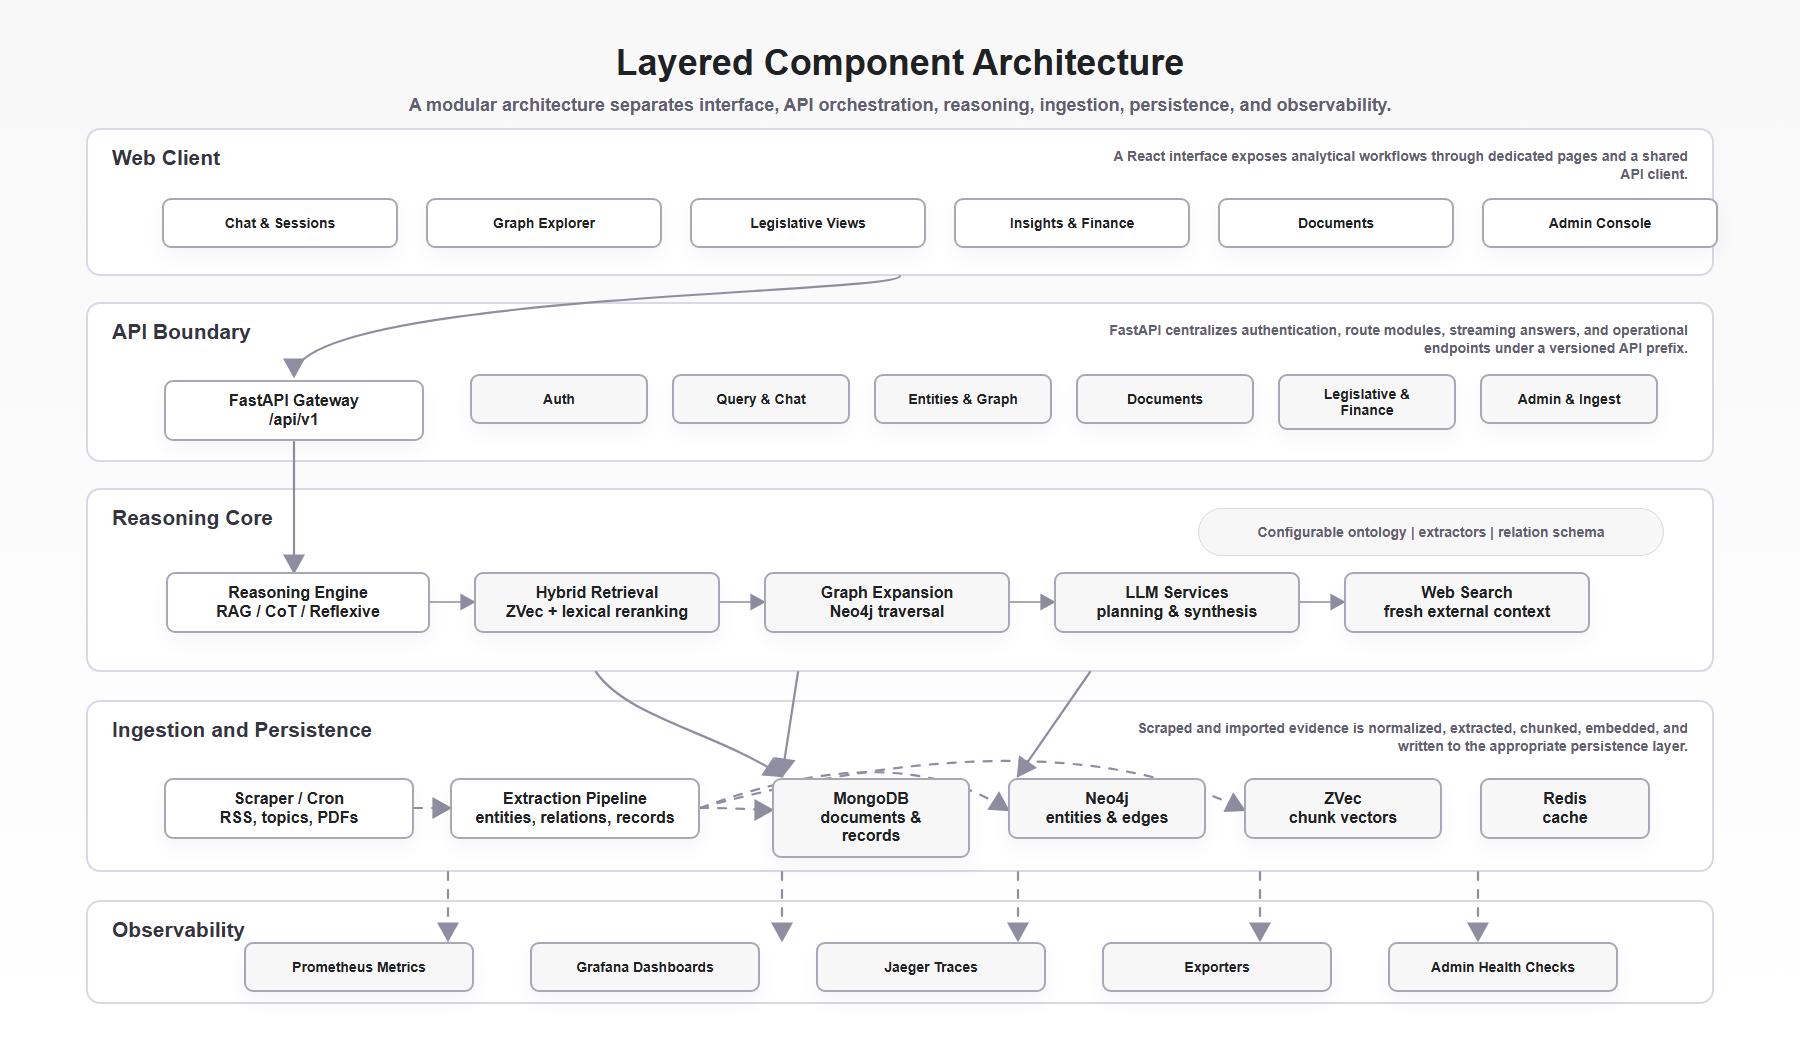
\includegraphics[width=0.96\textwidth,height=0.78\textheight,keepaspectratio]{images/component_architecture.png}
    \caption{Logical component architecture and separation of pipeline responsibilities.}
    \label{fig:component-architecture}
\end{figure}

\textbf{Hybrid evidence representation.} Political analysis requires both unstructured textual recall and structured relational precision. The design therefore maintains parallel representations: document-centric records and chunks for semantic search, canonical entities and typed edges for traversal, and structured analytical records (legislative, financial, conflict-oriented) where schema-specific views add value. Figure~\ref{fig:vector-vs-graph} contrasts the roles of vector space and graph space in the same query workflow. Vector retrieval contributes topical similarity and passage-level grounding; graph traversal contributes entity disambiguation, multi-hop paths, and temporal constraints. Neither store alone satisfies FR-04; the reasoning layer must fuse evidence from both modalities before synthesis (FR-07).

\begin{figure}[H]
    \centering
    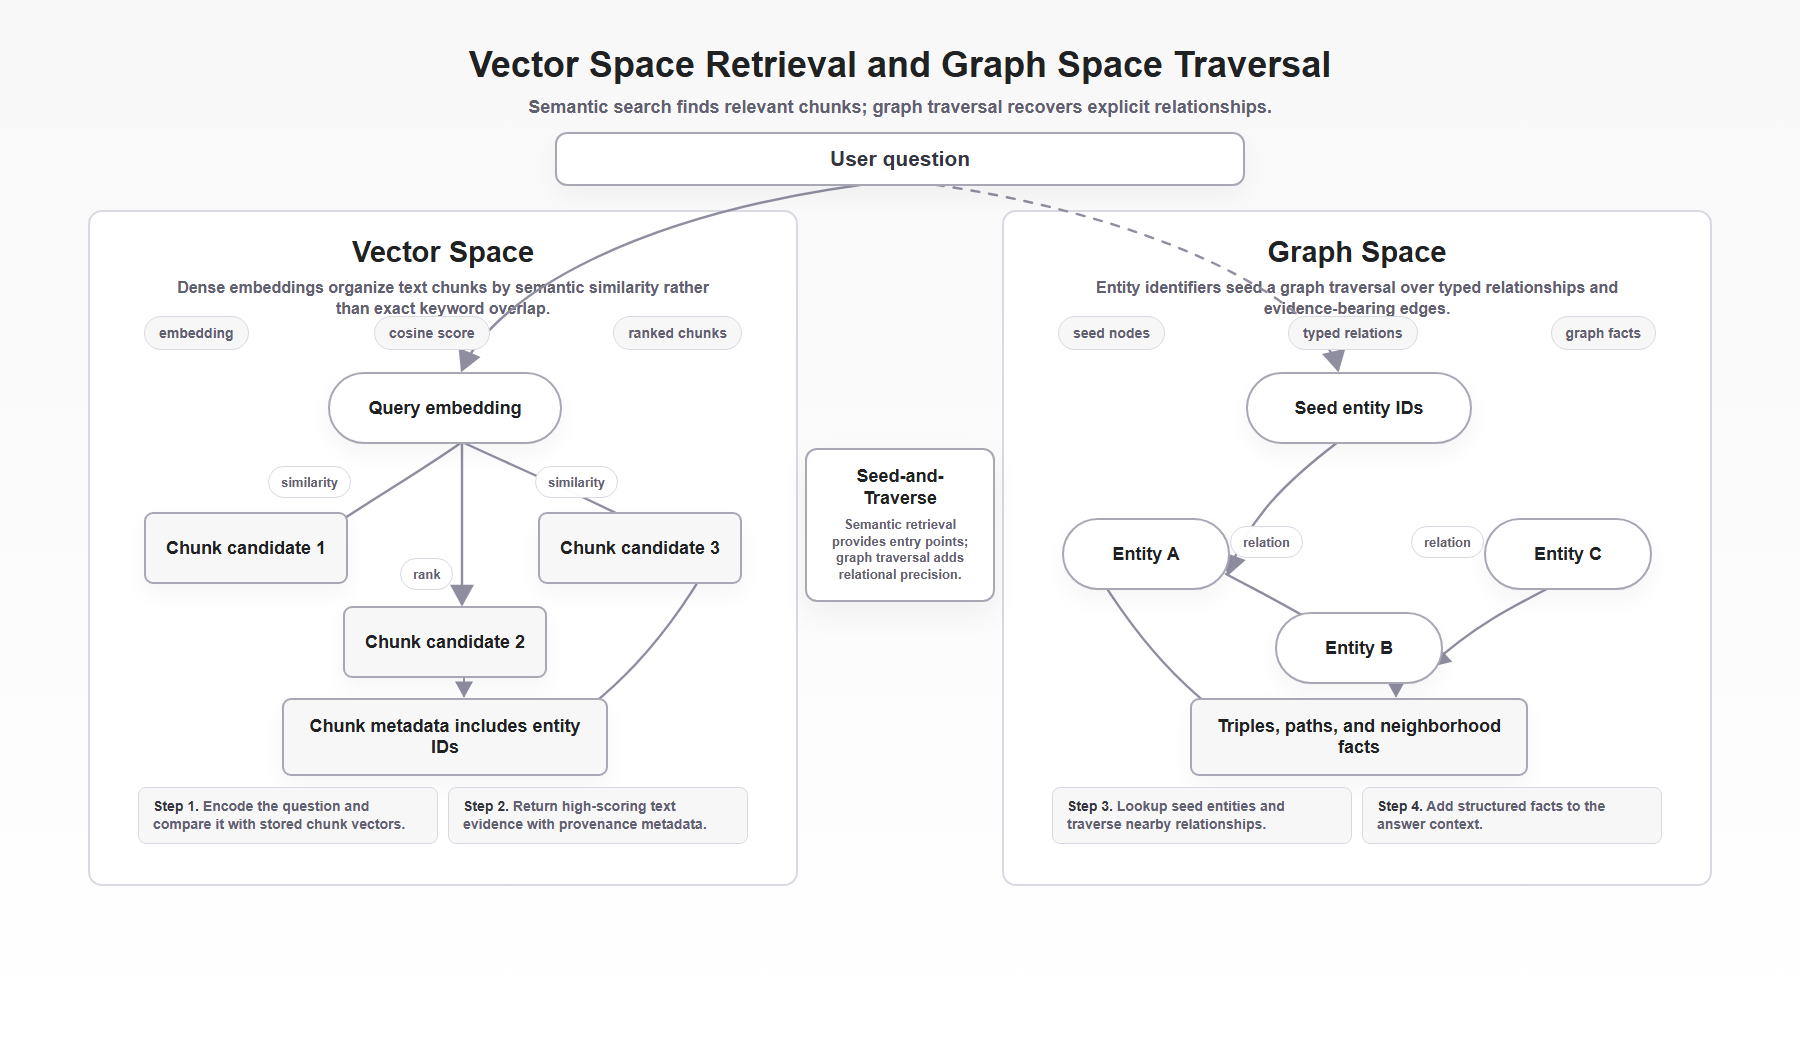
\includegraphics[width=0.96\textwidth,height=0.78\textheight,keepaspectratio]{images/vector_vs_graph_spaces.png}
    \caption{Complementary roles of vector retrieval and graph traversal in hybrid evidence access.}
    \label{fig:vector-vs-graph}
\end{figure}

\textbf{Traceability by design.} Every analytical output must remain linked to inspectable artifacts: source documents, chunk identifiers, graph nodes and edges used in traversal, and reasoning-step metadata exposed in the interface. Traceability is enforced at the data-model level (provenance fields on documents and assertions) and at the reasoning level (cited spans, graph-fact references, and optional audit loops in reflexive mode). This principle implements the validation criteria for reasoning and observability defined in Chapter~2.

\textbf{Evolvability and modularity.} Domain ontologies, extraction prompts, source connectors, and embedding settings may evolve during the internship and in later deployments. The architecture therefore treats MongoDB documents as the system of record for raw evidence and processing checkpoints, while Neo4j and ZVec hold derived views that can be rebuilt from documents without re-scraping sources. Containerized services and horizontal scaling of stateless workers (ingestion, API, reasoning) support growth in corpus size without redesigning the logical topology illustrated in Figure~\ref{fig:system-component-overview}. Observability (metrics, logs, traces) is treated as a cross-cutting concern rather than an afterthought, consistent with the non-functional requirements on auditability and operational diagnosis.

\begin{figure}[H]
    \centering
    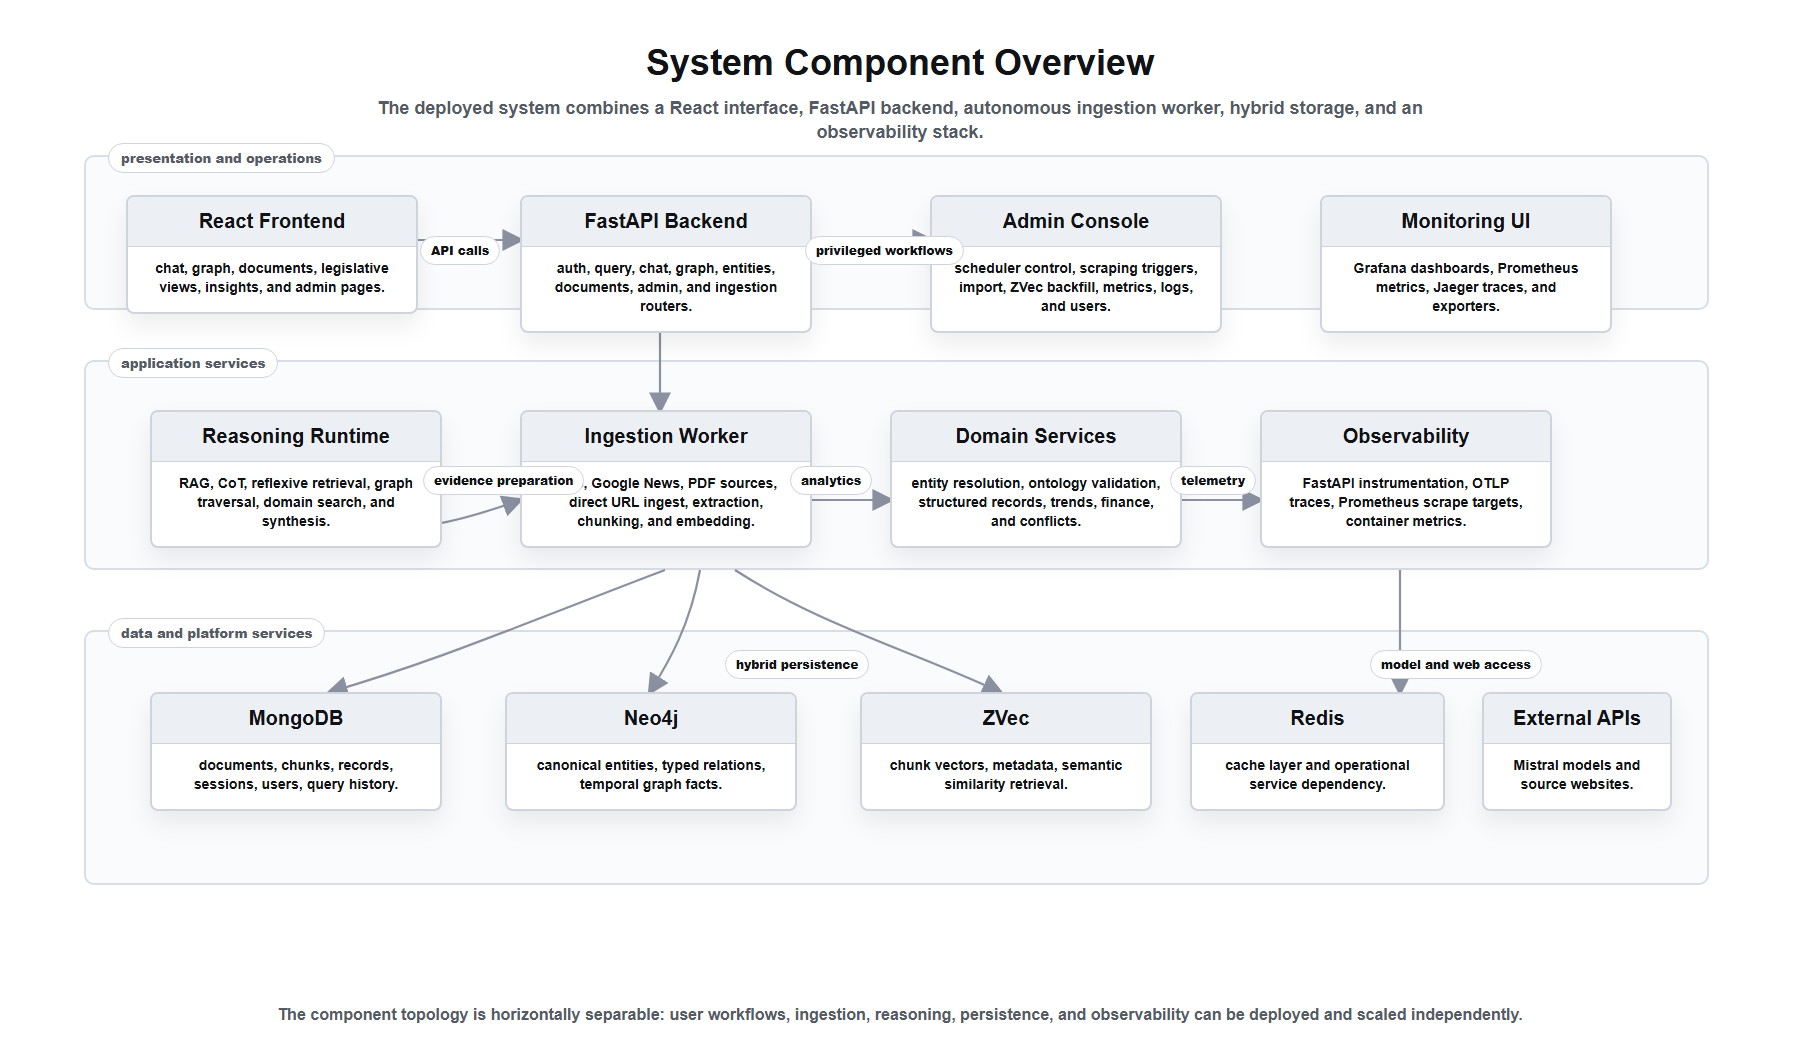
\includegraphics[width=0.96\textwidth,height=0.78\textheight,keepaspectratio]{images/system_component_overview.png}
    \caption{System component overview for ingestion, persistence, reasoning, and observability.}
    \label{fig:system-component-overview}
\end{figure}

\section{Use Case Refinement}

Chapter~2 introduced actors and primary use cases at requirement level. The detailed model refined here guided API and frontend boundaries. Authenticated users interact through cited question answering (with selectable reasoning depth), chat history, graph exploration, document library consultation, legislative and financial dashboards, trend and conflict views, and entity comparison. Each analytical workflow consumes prepared evidence from MongoDB, Neo4j, and ZVec rather than triggering full ingestion at query time; live web supplementation applies only when configured for recent events not yet indexed locally.

The system administrator supervises scheduler configuration, scraping and backfill jobs, ingestion log inspection, user management, health metrics, and selective reindexing of derived artifacts. Operational routes are isolated from standard analytical navigation through role-based access control in the frontend and privileged backend endpoints, so infrastructure actions are not conflated with everyday analytical sessions. Access control is modeled as a strict boundary between \emph{user} and \emph{administrator} roles: analytical capabilities require authentication, while administrative capabilities require an elevated role verified on both client and server.

Figure~\ref{fig:detailed-use-case} formalizes the use cases attached to each side of this boundary and aligns them with the implemented route structure. The model clarifies that graph exploration and document inspection are peer workflows to chat-based questioning, not secondary features. Administrative use cases (scheduler control, scraping supervision, reindexing) operate on the same evidence pipeline but must not bypass quality gates or idempotency rules defined for ingestion.

\begin{figure}[H]
    \centering
    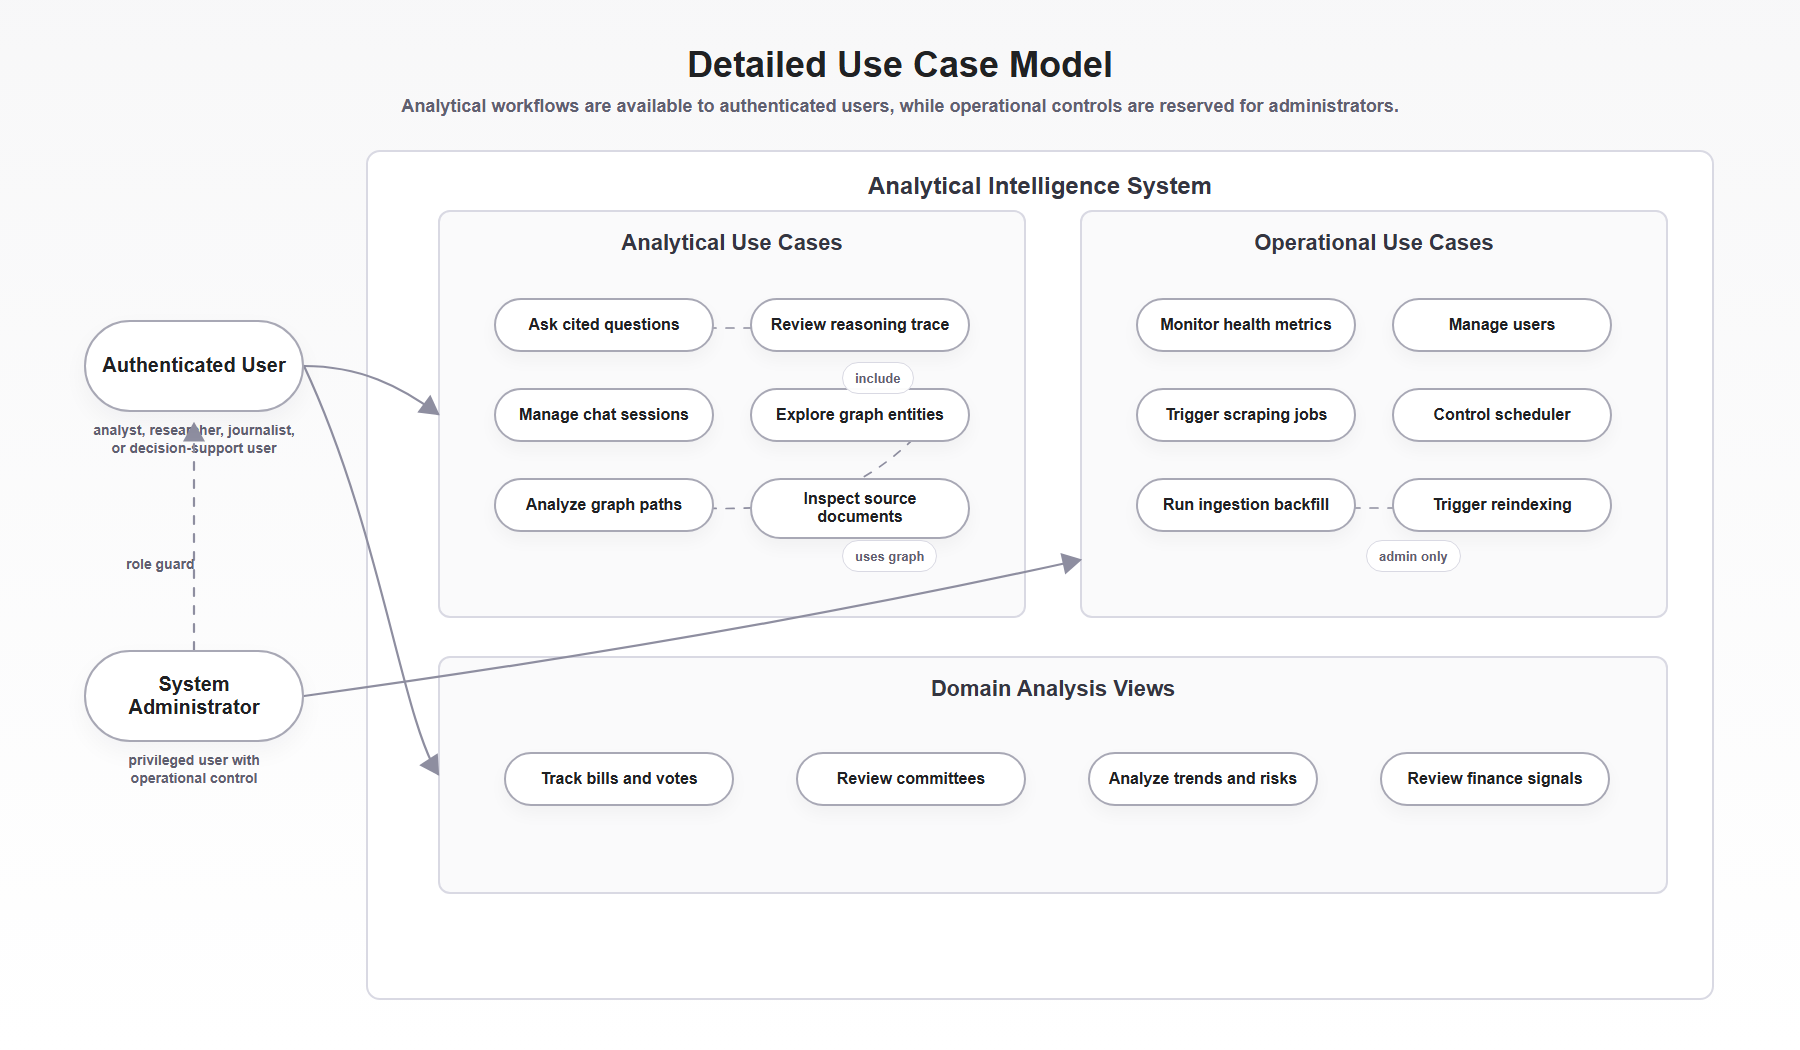
\includegraphics[width=0.96\textwidth,height=0.78\textheight,keepaspectratio]{images/detailed_use_case.png}
    \caption{Detailed use case model for analytical and administrative workflows.}
    \label{fig:detailed-use-case}
\end{figure}

\section{Data Flow Architecture}

The platform distinguishes \textbf{offline} evidence construction from \textbf{online} query-time reasoning. Offline flows prepare documents, structured records, graph topology, and vectors; online flows consume those artifacts under latency constraints suitable for interactive analysis.

External sources (RSS feeds, web articles, Google News topics, direct URLs, PDF reports) enter through the acquisition layer and are normalized into MongoDB documents with source metadata and processing flags. Quality gating rejects unsuitable content before extraction. Accepted documents pass through graph extraction (entities and relations to Neo4j; mentions and assertions in MongoDB), structured extraction (domain records such as bills, votes, committees, contributions, conflict flags), and chunking with embedding into ZVec. Checkpoint flags on each document make the offline sequence resumable and idempotent.

At query time, a request arrives at the FastAPI endpoint with parameters for reasoning mode, hop limit, and optional web search. The reasoning engine retrieves ZVec chunks and Neo4j paths (and structured records when the planner requests them), fuses evidence, and invokes synthesis with citation metadata. The response returns answer text, sources, graph facts, traces, and confidence signals for the frontend. Online flow does not mutate the corpus except through explicit administrative ingestion triggers.

Figure~\ref{fig:data-flow-diagram} consolidates both paths from external sources to cited answers. The diagram emphasizes responsibility splits: MongoDB holds documents and derived textual artifacts; Neo4j holds canonical relational topology; ZVec holds embedded chunks linked to document and entity identifiers. Query execution reads from all three stores but writes only to session and history collections unless an administrator launches ingestion.

\begin{figure}[H]
    \centering
    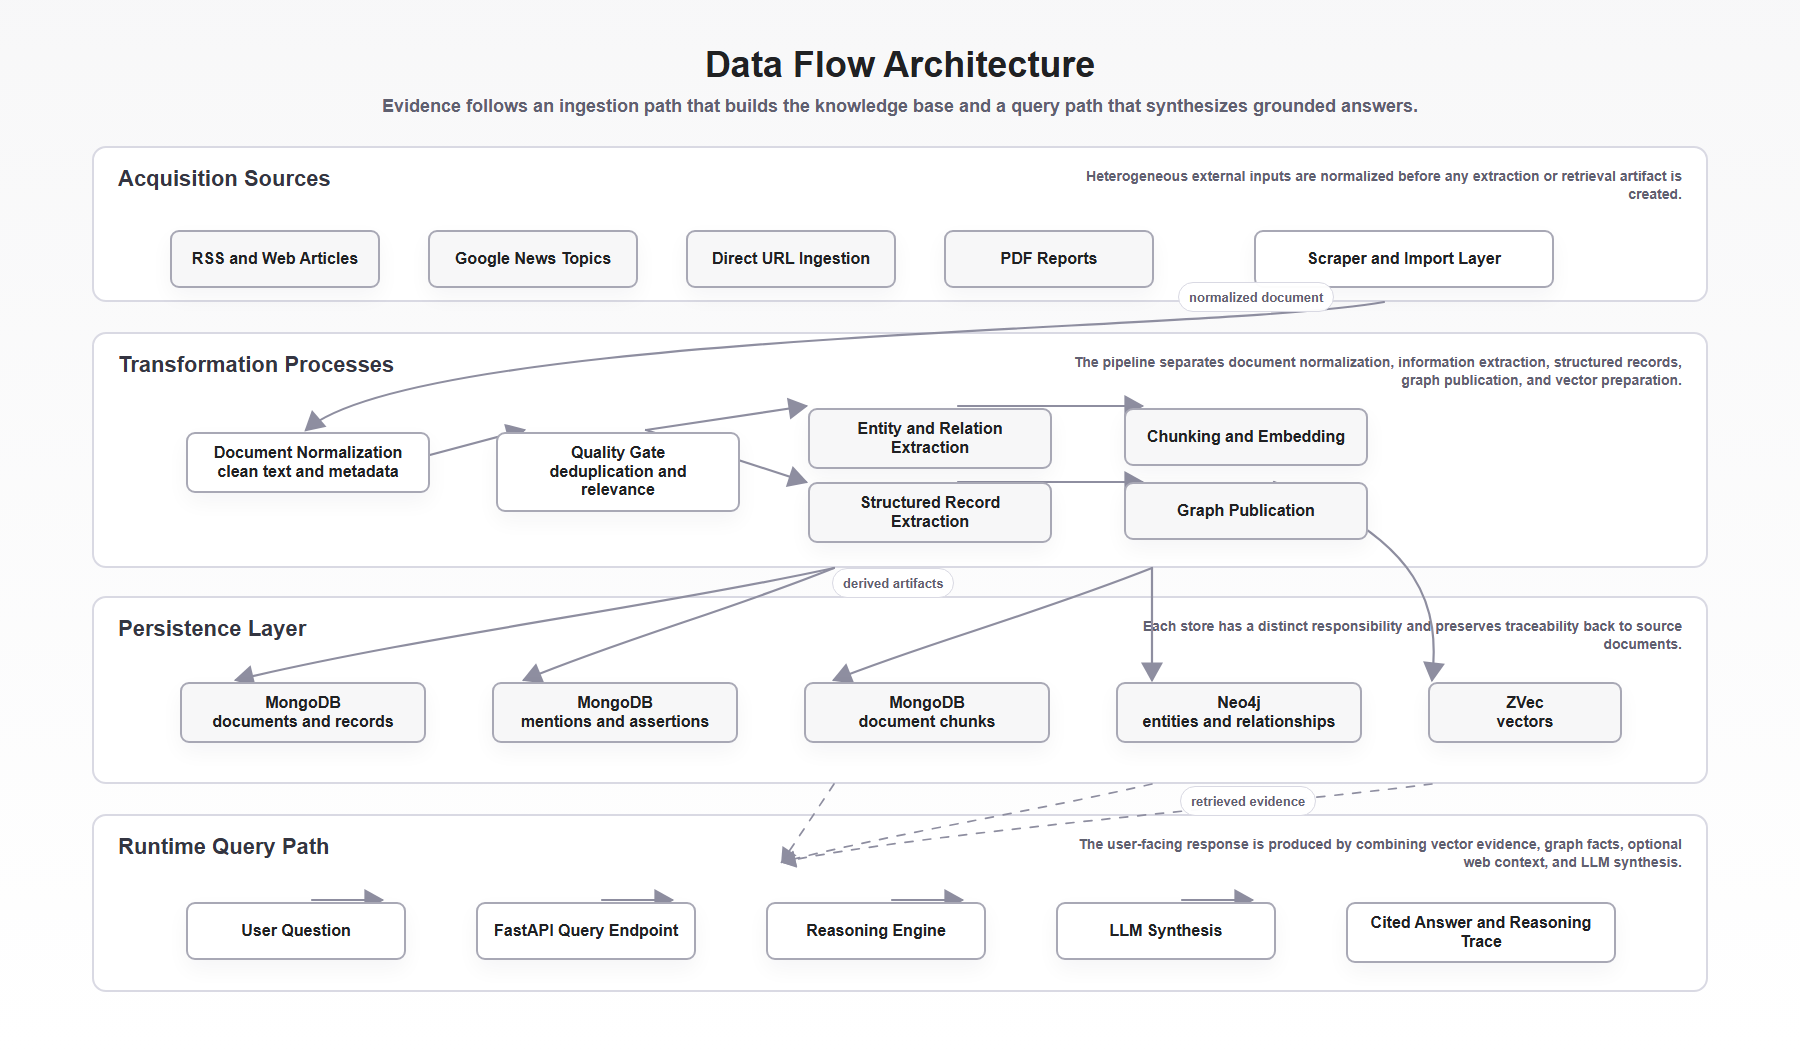
\includegraphics[width=0.96\textwidth,height=0.78\textheight,keepaspectratio]{images/data_flow_diagram.png}
    \caption{Data flow architecture from acquisition to grounded answer generation.}
    \label{fig:data-flow-diagram}
\end{figure}

\section{Ingestion Architecture}

Ingestion implements FR-01, FR-08, FR-09, and FR-10 through a multi-level acquisition strategy, explicit normalization and quality gates, and a document-level state machine.

The ingestion engine combines three complementary levels rather than a single crawler template. \textbf{Level~1} monitors a curated registry of \textbf{57 high-precision outlets} on schedules (RSS, institutional portals, known political feeds). \textbf{Level~2} extends coverage with query-driven deep discovery for thematic gaps (search, link traversal, dynamic rendering, pagination). \textbf{Level~3} handles unstructured documents such as PDF reports through high-fidelity parsers that preserve layout and tables. Figure~\ref{fig:autonomous-crawler-final} summarizes the pipeline from collection to retrieval-ready artifacts. Discovery, extraction, normalization, and quality control remain separate stages so new source families can be added without rewriting the reasoning engine.

\begin{figure}[H]
    \centering
    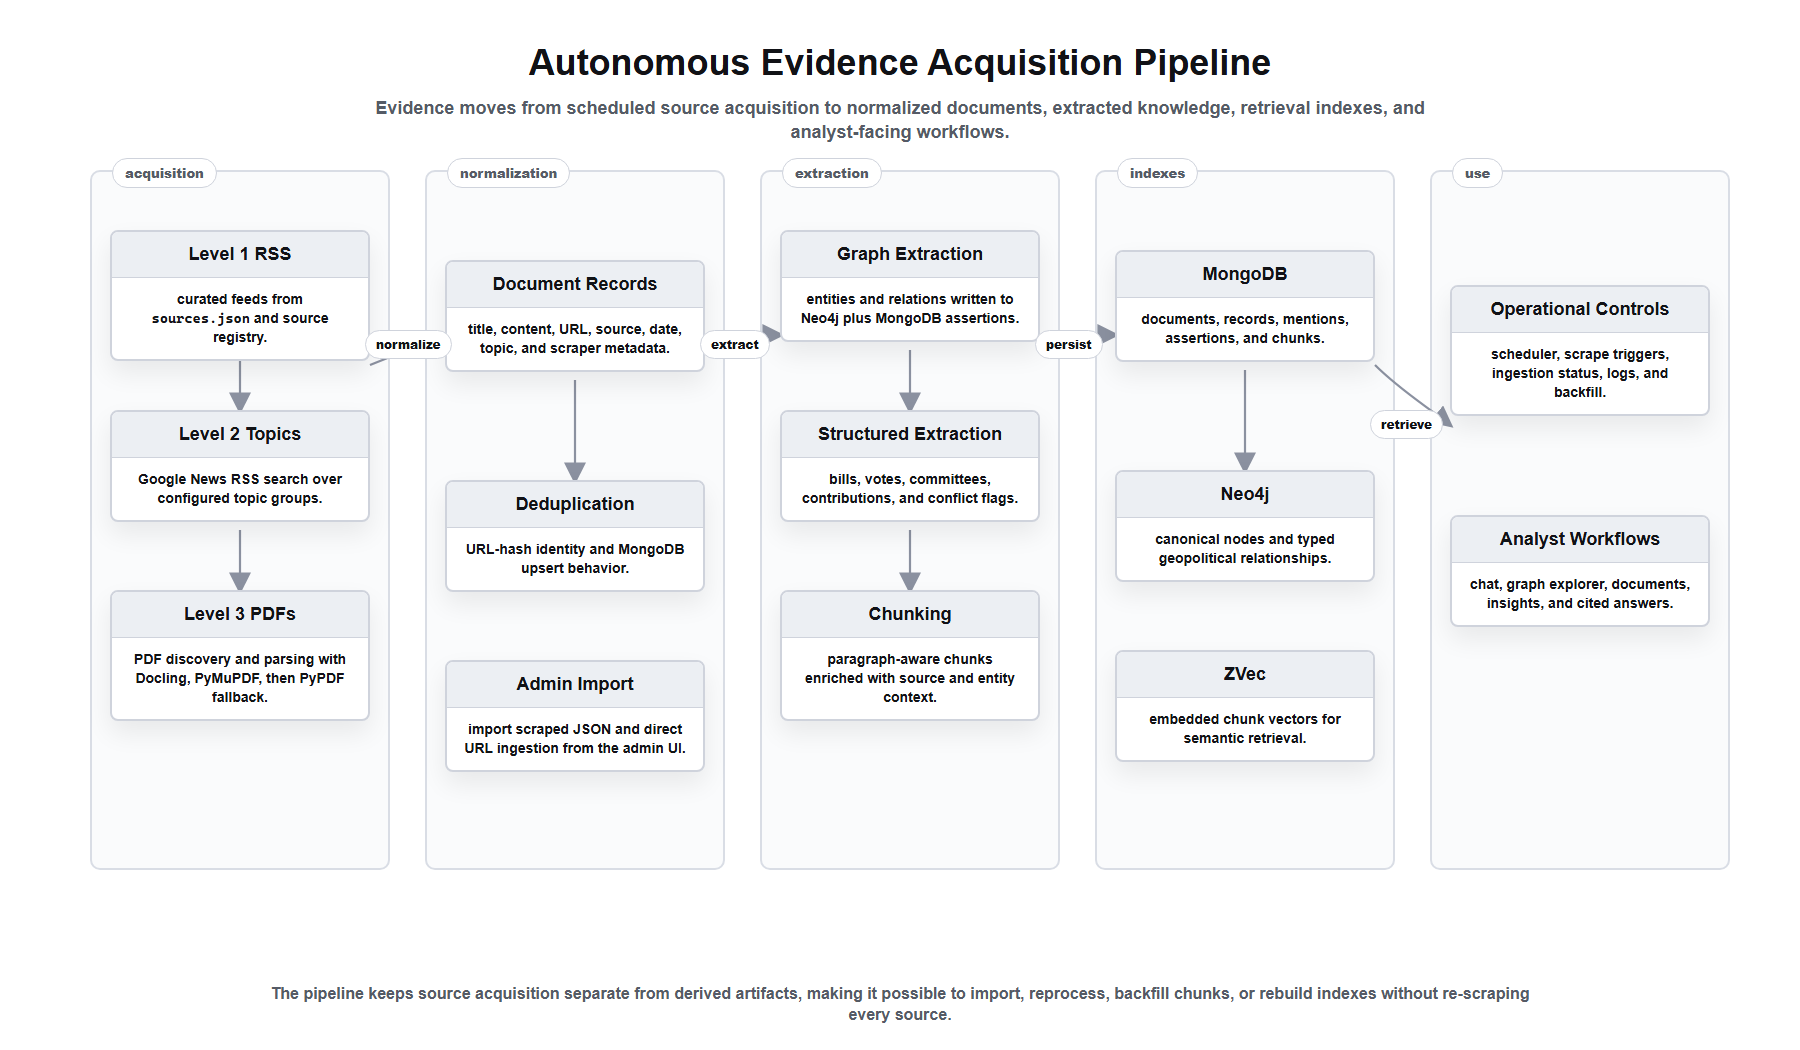
\includegraphics[width=0.96\textwidth,height=0.78\textheight,keepaspectratio]{images/autonomous_crawler_pipeline.png}
    \caption{Autonomous evidence acquisition pipeline from source collection to retrieval-ready artifacts.}
    \label{fig:autonomous-crawler-final}
\end{figure}

All acquired content converges on a unified document schema: identifiers, timestamps, provenance, language hints, and normalized body text. Quality gates filter documents whose length, metadata, or topical signal fall below thresholds for reliable extraction; rejected items remain logged for administrator review without polluting graph or vector indexes. Normalization is the prerequisite for deduplication and for consistent joint extraction (FR-02).

The document lifecycle is modeled as an explicit state machine with checkpoints rather than a monolithic ingest operation. Flags such as \texttt{graph\_extracted}, \texttt{structured\_extracted}, and \texttt{chunks\_created} record completion of each derived stage so that partial reprocessing is possible when prompts, schemas, or embeddings change. Figure~\ref{fig:state-document-lifecycle} shows transitions from raw acquisition through quality gating to graph publication, structured records, and vector indexing. Explicit states improve operational control: the pipeline can resume after interruption, skip completed work, or rebuild only derived layers without re-scraping originals.

\begin{figure}[H]
    \centering
    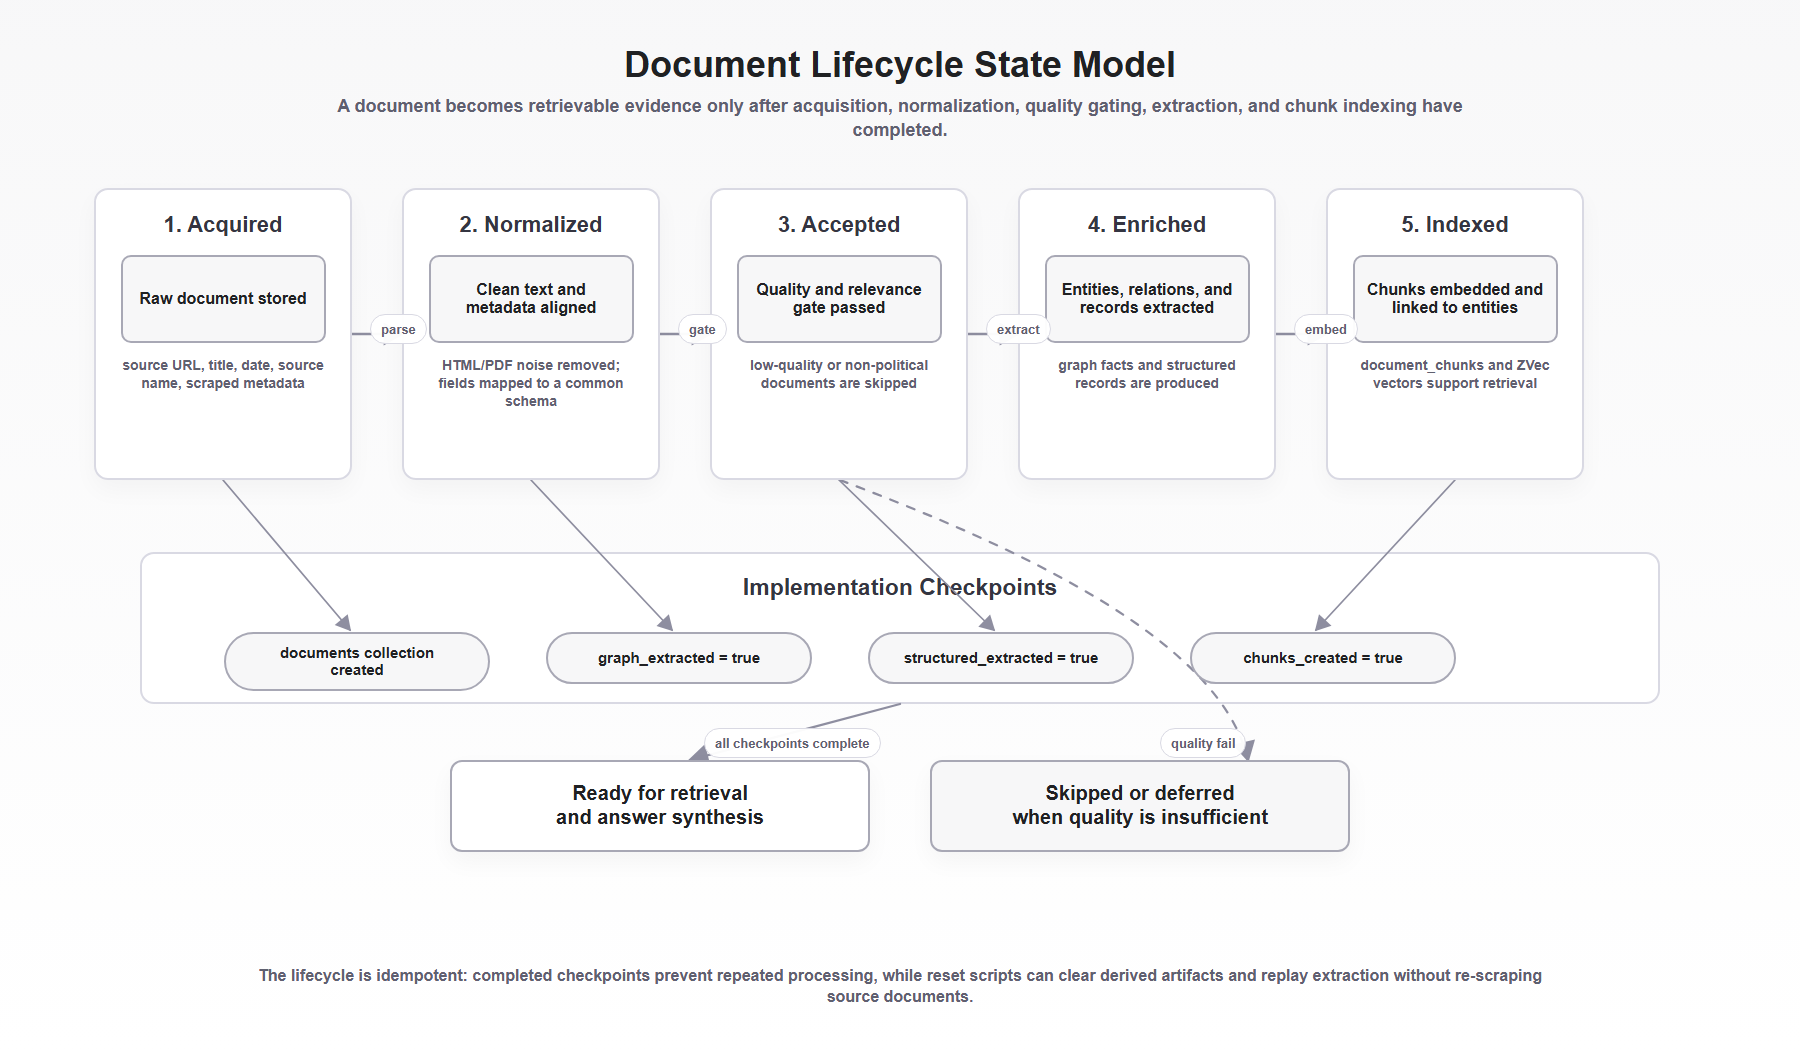
\includegraphics[width=0.96\textwidth,height=0.78\textheight,keepaspectratio]{images/state_document_lifecycle.png}
    \caption{Document lifecycle and ingestion checkpoints before retrieval.}
    \label{fig:state-document-lifecycle}
\end{figure}

\section{Knowledge Representation and Ontology}

The knowledge layer centers on a geopolitical property graph supplemented by document-grounded structured records and vectorized chunks.

The Neo4j ontology defines canonical node types including \texttt{POLITICIAN}, \texttt{PARTY}, \texttt{ORGANIZATION}, \texttt{INSTITUTION}, \texttt{EVENT}, and related geopolitical categories. Approximately \textbf{32 typed relation families} cover actor ties, geopolitical links, events, financial or influence relations, and evidence-backed assertions. Entity resolution maps surface mentions to stable canonical identifiers so syndicated or variant spellings do not fragment the graph. Figure~\ref{fig:class-domain-model} links graph topology to MongoDB evidence objects and ZVec chunks: bills, votes, contributions, and conflict flags remain document-grounded structured data in MongoDB, while actors, institutions, places, and events form traversable graph structure in Neo4j.

\begin{figure}[H]
    \centering
    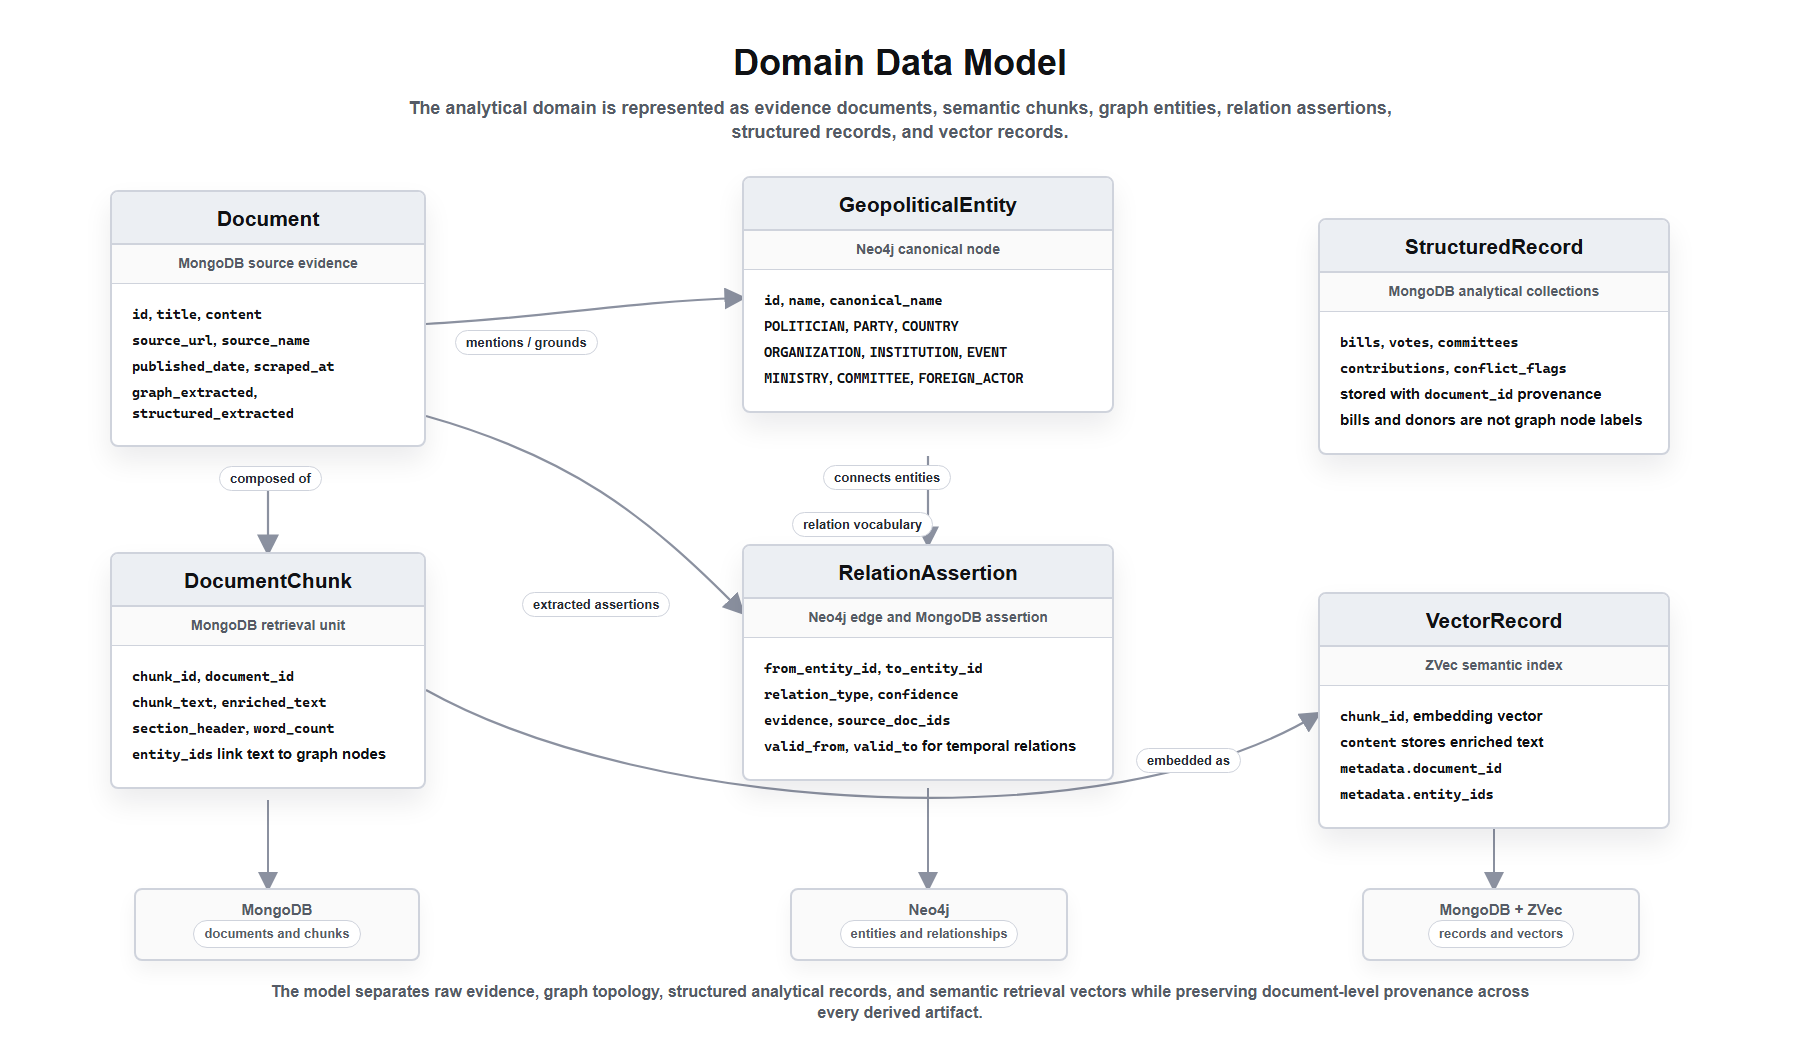
\includegraphics[width=0.96\textwidth,height=0.78\textheight,keepaspectratio]{images/class_domain_model.png}
    \caption{Domain data model linking evidence, graph topology, structured records, and vector retrieval.}
    \label{fig:class-domain-model}
\end{figure}

Political relations are time-bounded: office holding, alliances, and opposition change with elections, conflicts, and institutional reform. Where chronology is available, edges carry \texttt{valid\_from} and \texttt{valid\_to} attributes so queries can reconstruct states valid at a requested period rather than mixing obsolete and current facts. Temporal attributes support trend, conflict, and comparative use cases from Chapter~2 and condition multi-hop answers on FR-06.

Provenance is anchored on the \texttt{documents} collection: each chunk, mention, assertion, and structured record references its source document and extraction pass. Graph edges in Neo4j remain traceable to assertions stored in MongoDB before publication. This dual linkage satisfies traceability by design and enables the citation layer in the reasoning architecture.

\section{Data Model and Physical Schema}

Persistence is deliberately polyglot: a document store for evidence and operational metadata, a graph store for relational traversal, and a vector store for semantic recall.

MongoDB is the system of record for raw and derived textual evidence. Core collections include \texttt{documents} (provenance and processing state), \texttt{document\_chunks}, entity \texttt{mentions}, relation \texttt{assertions}, and domain-specific structured collections (legislative, financial, conflict). Application collections (\texttt{users}, chat \texttt{sessions}, \texttt{messages}, query \texttt{history}) are separated from evidence collections so that user activity does not complicate corpus rebuilds. Figure~\ref{fig:graph-vs-relational} motivates the document-centric primary store versus graph specialization: document storage preserves full text, extraction artifacts, and flexible schemas for heterogeneous political sources, while the graph store optimizes typed traversal and disambiguation rather than replacing document provenance.

\begin{figure}[H]
    \centering
    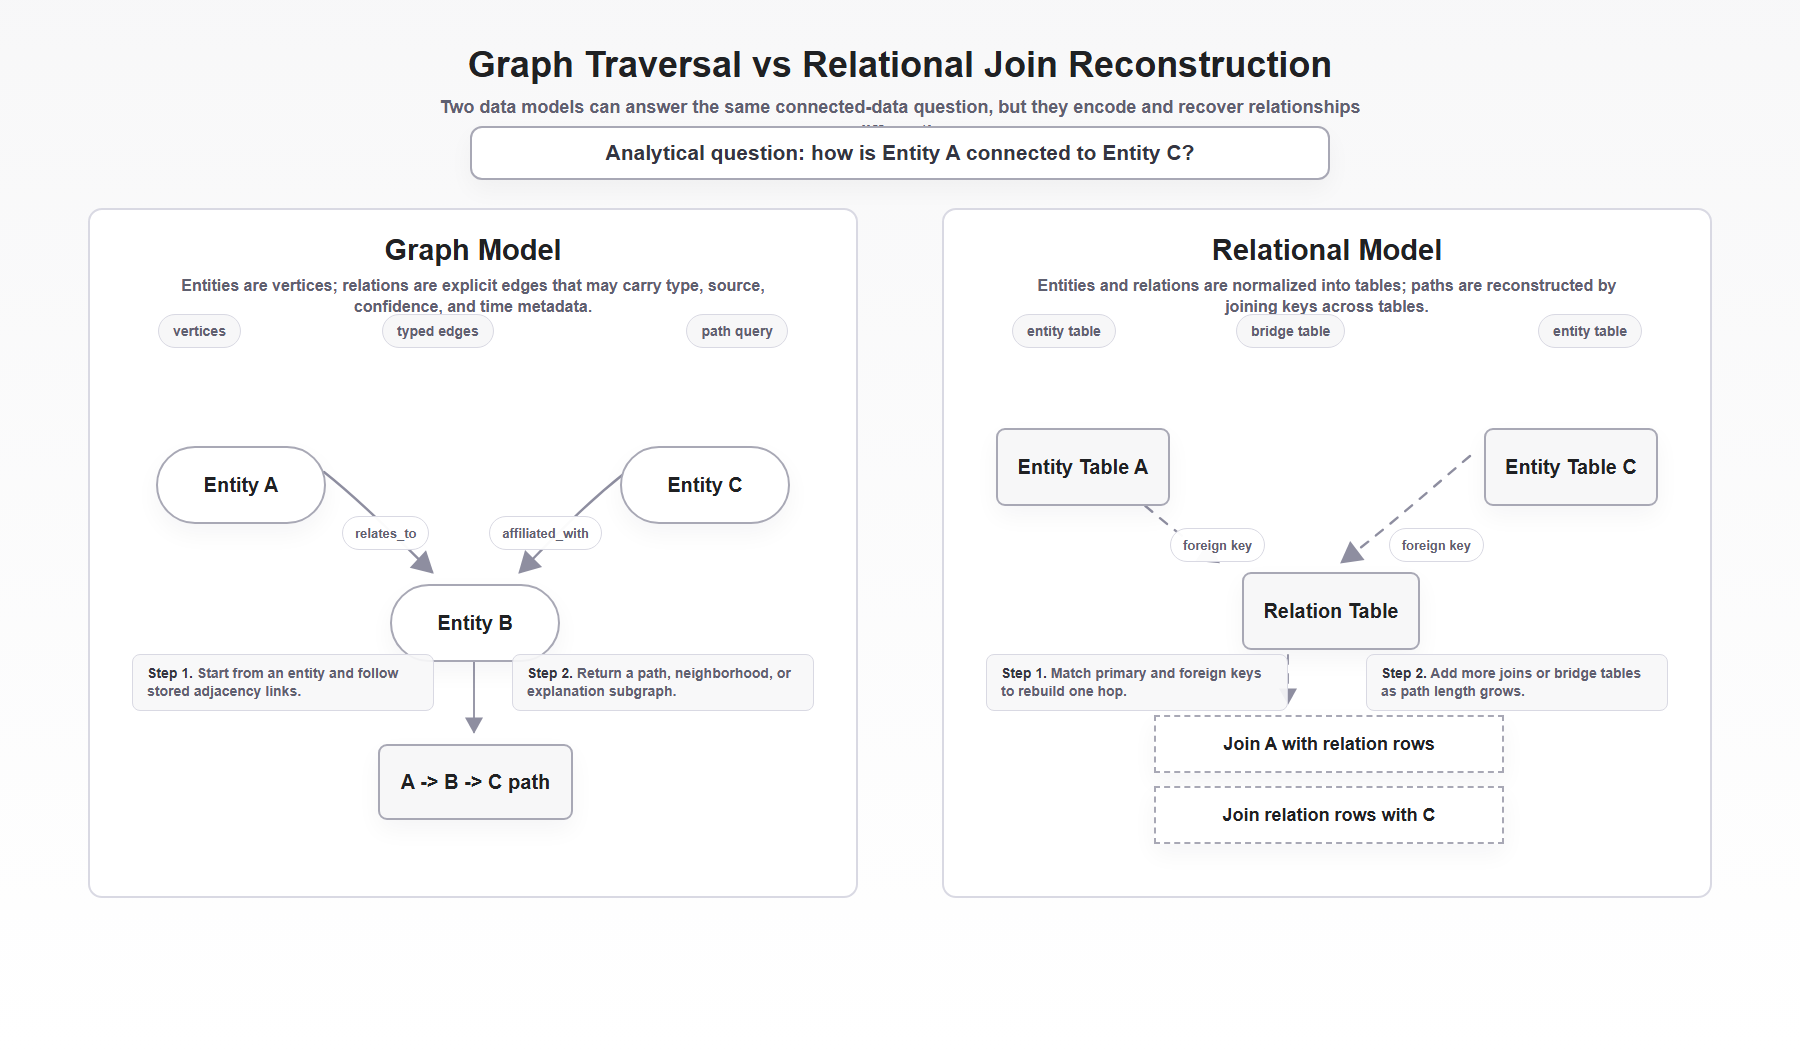
\includegraphics[width=0.96\textwidth,height=0.78\textheight,keepaspectratio]{images/graph_vs_relational.png}
    \caption{Document-centric evidence storage versus graph-native relational queries.}
    \label{fig:graph-vs-relational}
\end{figure}

Neo4j holds canonical entities and typed relationships produced after resolution and validation. The schema is optimized for multi-hop queries up to the performance target defined in Chapter~2 (approximately three hops under nominal load). Indexes and relationship types align with the ontology categories above; temporal attributes are applied on edges when evidence supports interval bounds.

ZVec stores dense embeddings of \texttt{document\_chunks} with metadata linking chunk identifiers, document identifiers, and associated entity identifiers where available. Vector records enable semantic recall in hybrid search (FR-04) and feed the first hop of standard RAG mode. Re-embedding can be executed independently of graph republication when only the embedding model changes.

Figure~\ref{fig:database-erd} presents the integrated physical view across MongoDB, Neo4j, and ZVec, including runtime collections for authentication and chat. The ERD clarifies that \texttt{documents} sit at the center of provenance links to chunks, structured records, and extraction artifacts, while Neo4j and ZVec remain rebuildable derived stores.

\begin{figure}[H]
    \centering
    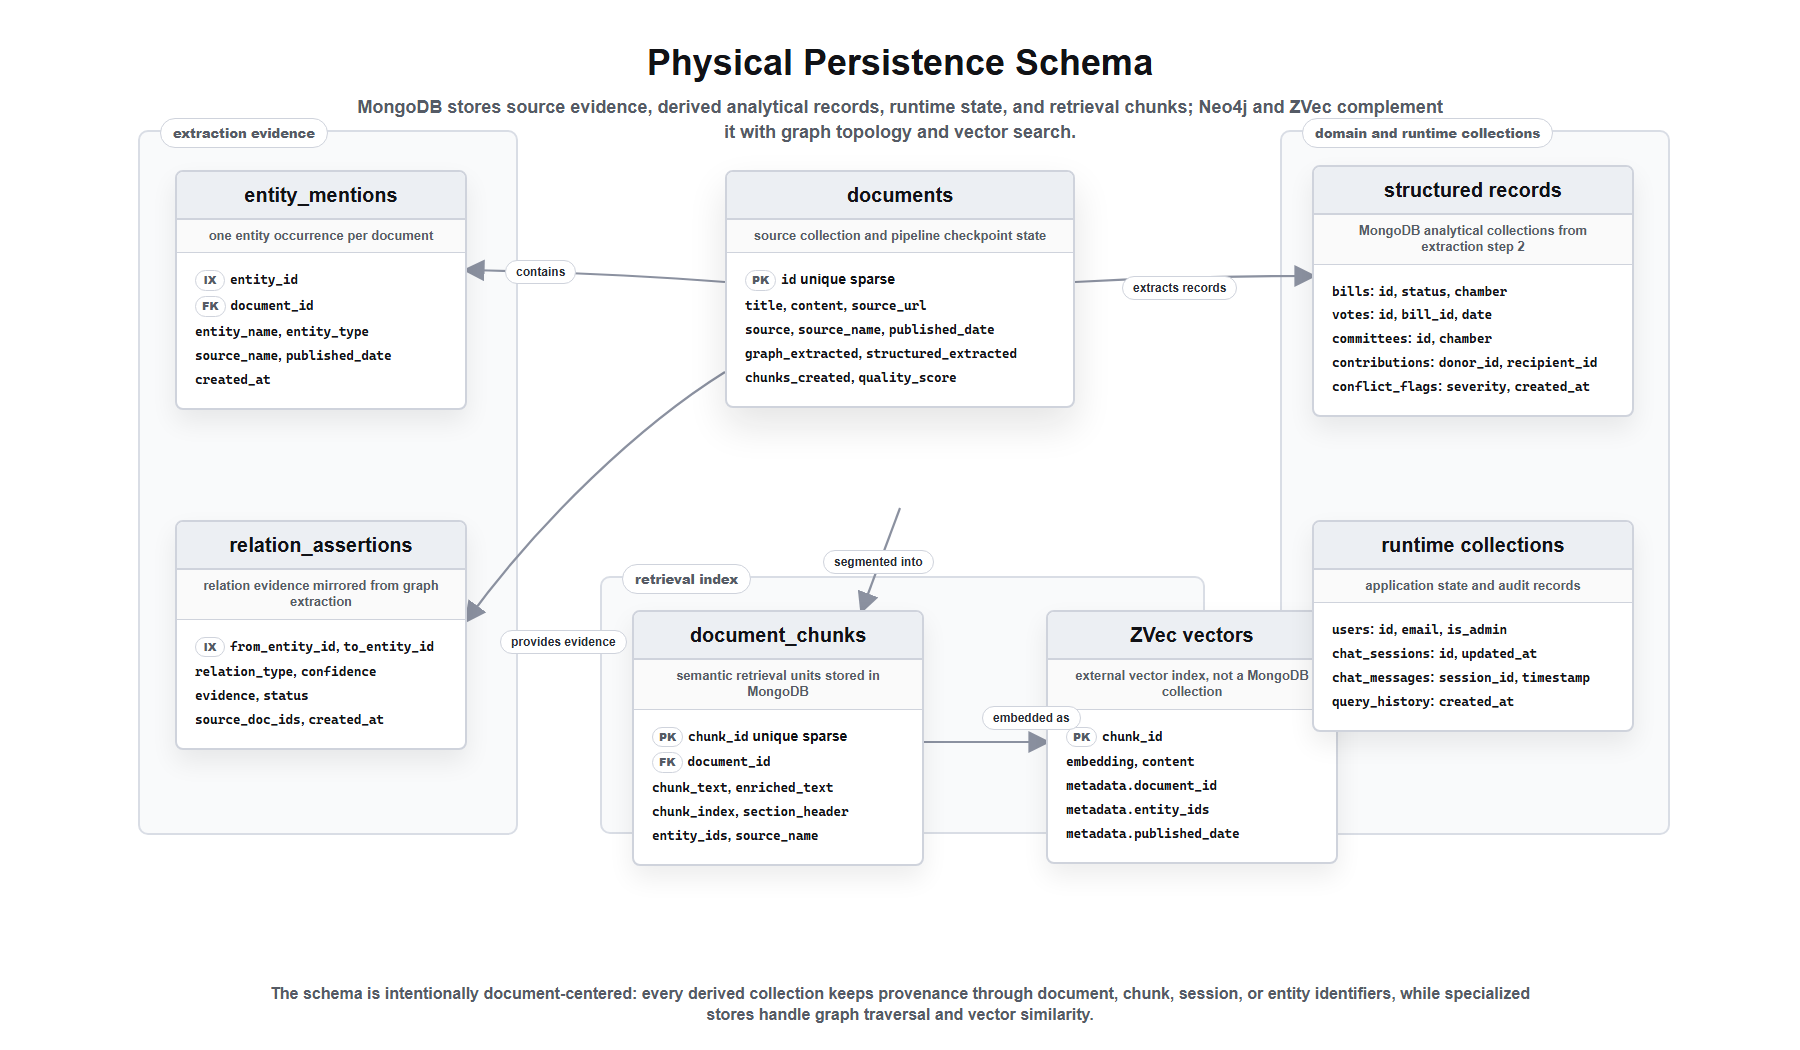
\includegraphics[width=0.96\textwidth,height=0.78\textheight,keepaspectratio]{images/database_erd.png}
    \caption{Physical persistence schema across MongoDB, Neo4j, and ZVec.}
    \label{fig:database-erd}
\end{figure}

\section{Reasoning Architecture}

The reasoning layer implements FR-04, FR-05, and FR-07 through a plan--retrieve--synthesize loop with selectable modes and explicit evidence fusion.

At design level, each query iteration performs three stages. \textbf{Planning} interprets the question and, in multi-hop modes, decomposes sub-questions or selects seed entities. \textbf{Retrieval} fetches ZVec chunks, Neo4j paths, and optional structured records. \textbf{Synthesis} generates a cited answer from fused context. Reflexive mode adds an audit step that tests evidence sufficiency and may trigger additional hops up to \textbf{MAX\_HOPS = 3}. Optional live web search supplements the local corpus when configured for breaking events not yet ingested. Figure~\ref{fig:sequence-reasoning} shows interactions among the API, reasoning engine, persistence stores, and language model; the loop terminates when acceptance criteria for the selected mode are met or the hop limit is reached.

\begin{figure}[H]
    \centering
    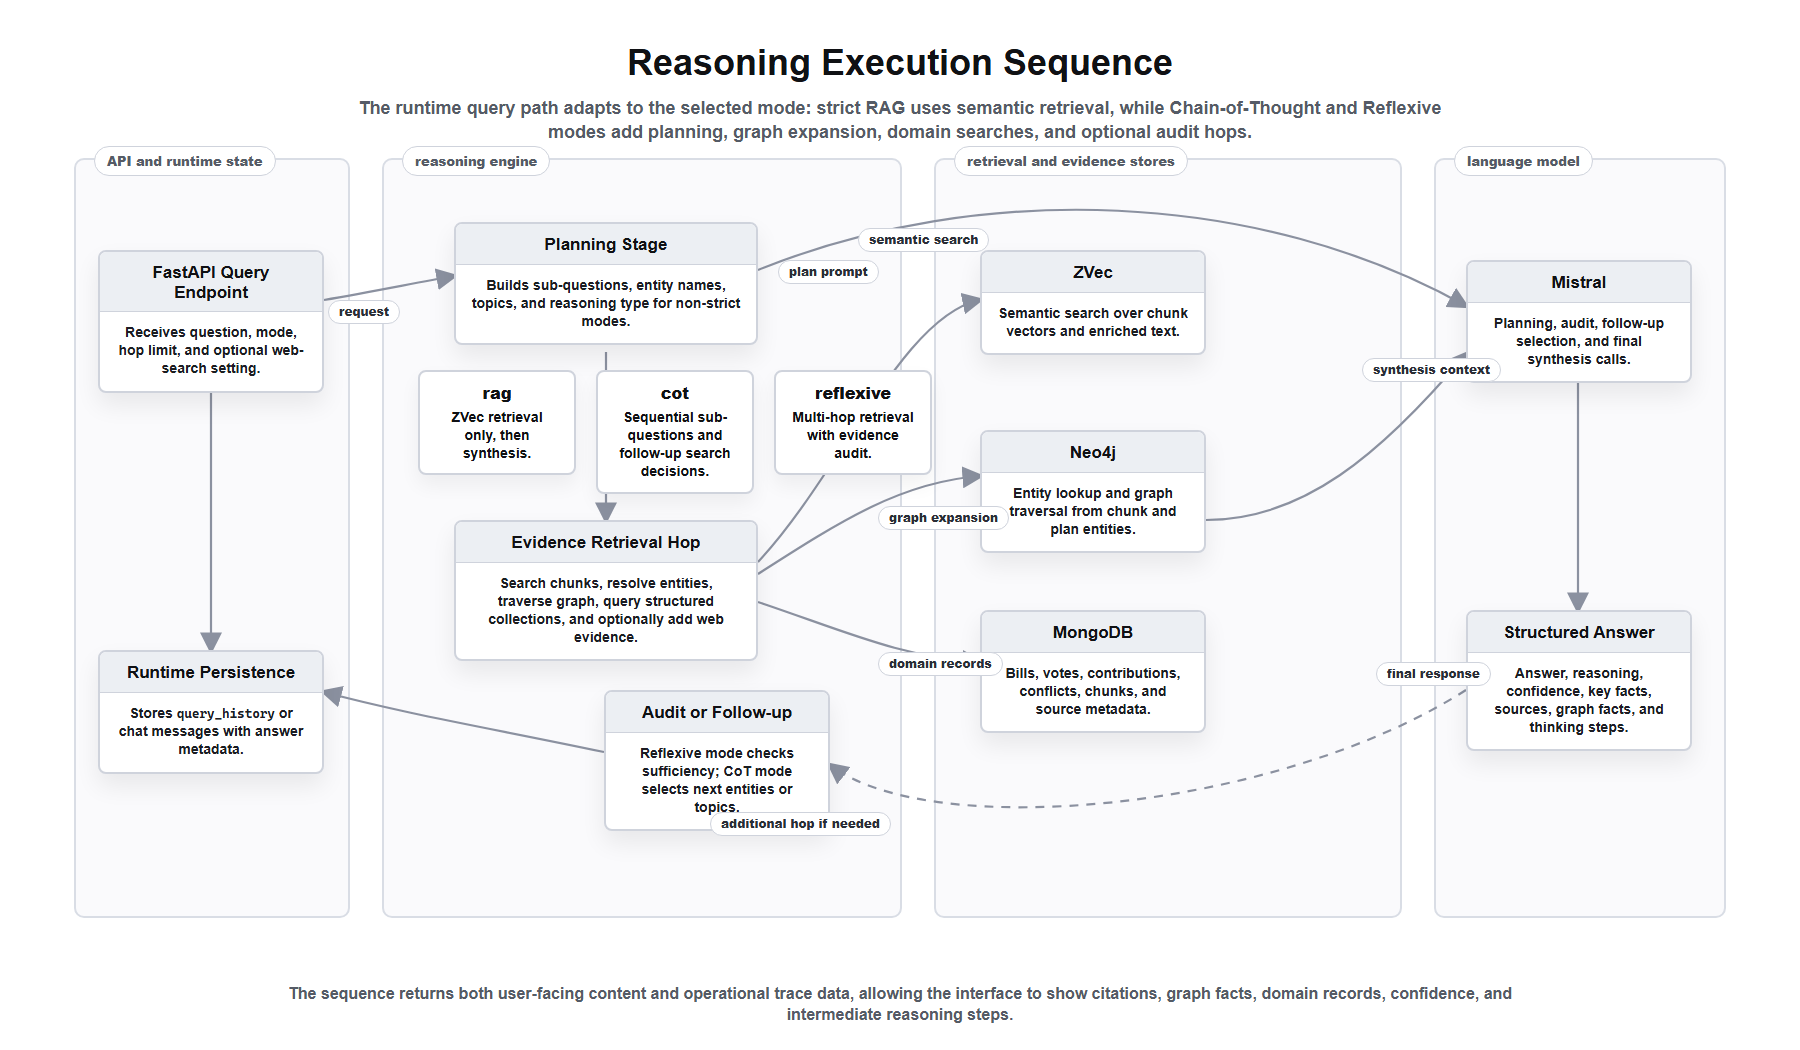
\includegraphics[width=0.96\textwidth,height=0.78\textheight,keepaspectratio]{images/sequence_reasoning.png}
    \caption{Reasoning execution sequence across retrieval, graph expansion, audit, and synthesis.}
    \label{fig:sequence-reasoning}
\end{figure}

Three modes are exposed at query time, trading latency against analytical depth. \textbf{Standard RAG (\texttt{rag})} performs one-hop semantic retrieval from ZVec using the user question, then direct synthesis; it suits factual lookups with minimal latency. \textbf{Chain-of-thought (\texttt{cot})} decomposes complex questions into sub-queries and may follow entities or topics across hops before synthesis. \textbf{Reflexive (\texttt{reflexive})} evaluates completeness and consistency after retrieval; insufficient evidence triggers refined retrieval rather than immediate answer generation. Mode selection implements FR-05 at architecture level; Chapter~4 details the \texttt{ReasoningEngine} and DSPy orchestration. Interface-level traces expose steps to satisfy FR-07 regardless of mode.

Evidence fusion merges ranked chunks, graph facts (nodes, edges, paths), and relevant structured records into a single context package for the synthesizer. Ranking considers semantic score, graph distance to seed entities, temporal validity, and deduplication of syndicated passages. Conflicting assertions are passed with provenance so synthesis can qualify claims rather than collapse contradictions silently. Fusion rules are mode-dependent: standard RAG prioritizes chunk relevance; multi-hop modes weight graph expansion; reflexive mode may narrow retrieval targets after audit feedback.

Figure~\ref{fig:technical-class-diagram} summarizes the logical service layering (API routes, domain services, store connectors, model clients) that implements the reasoning and ingestion designs above. Persistence access is isolated from orchestration logic so stores can be mocked or replaced during testing and evolution.

\begin{figure}[H]
    \centering
    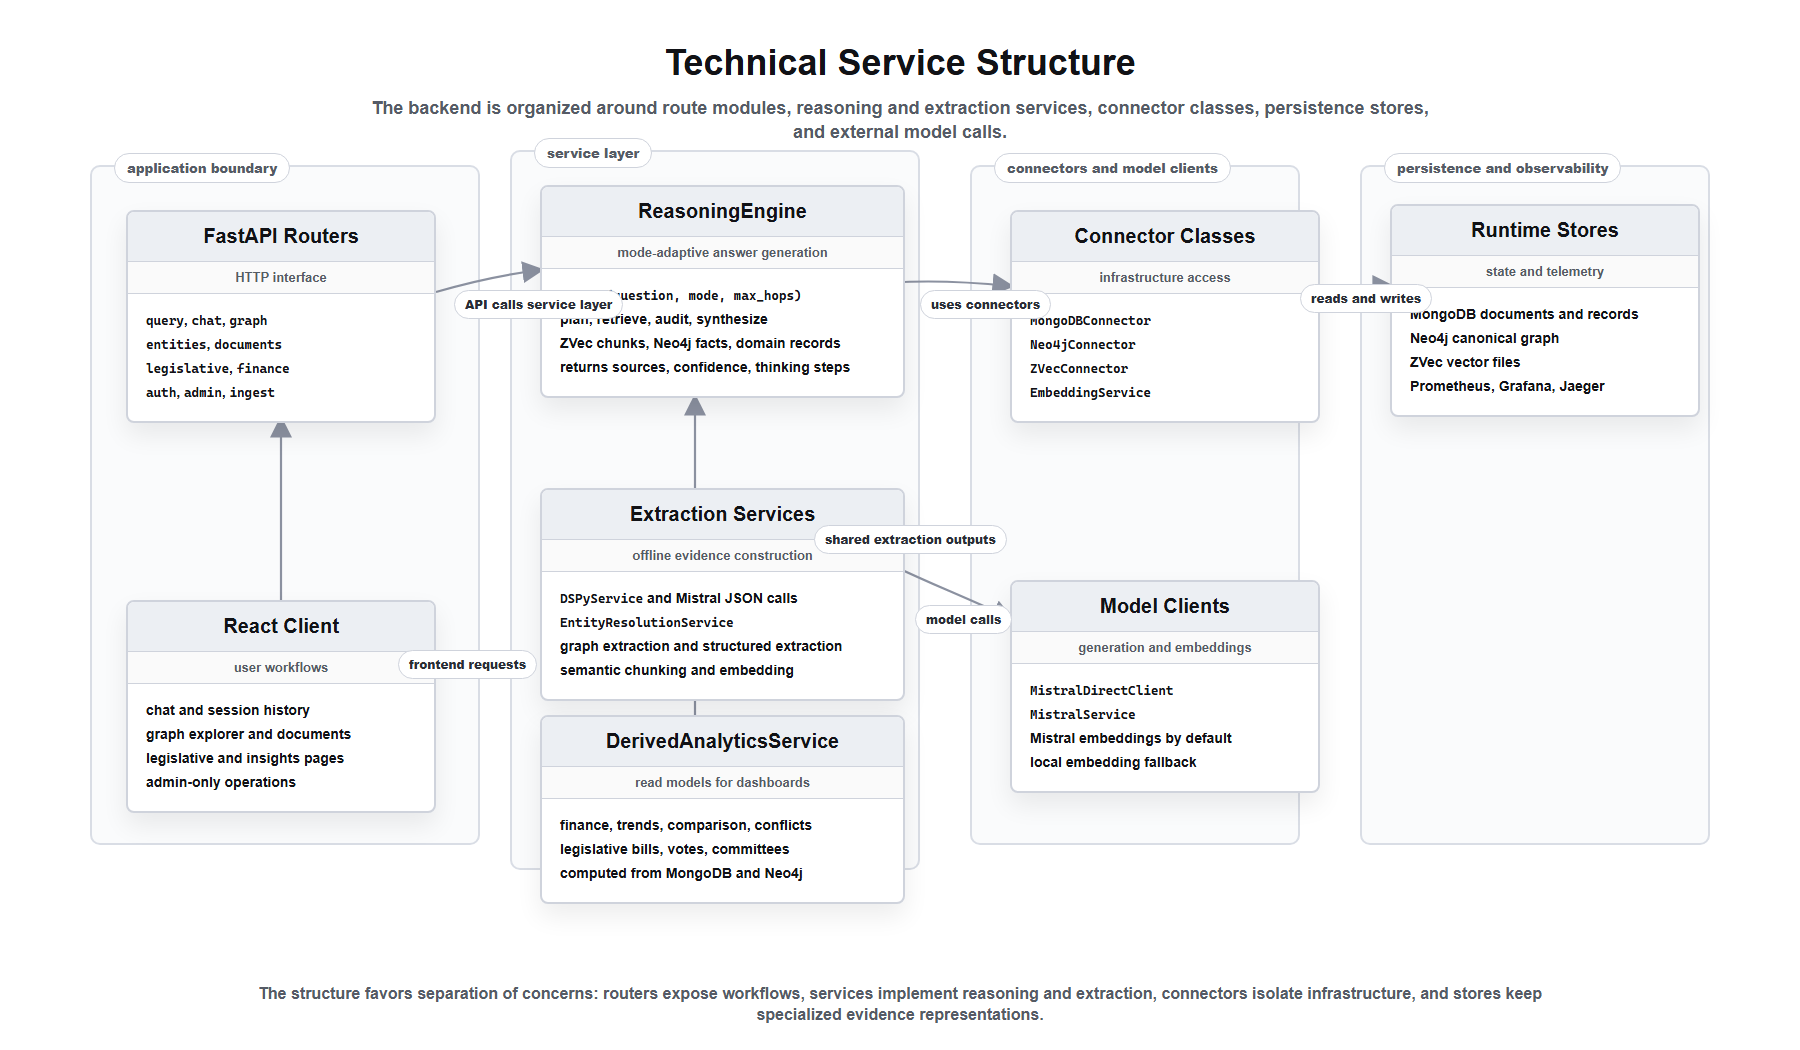
\includegraphics[width=0.96\textwidth,height=0.78\textheight,keepaspectratio]{images/technical_class_diagram.png}
    \caption{Technical service structure across API routes, services, connectors, stores, and model clients.}
    \label{fig:technical-class-diagram}
\end{figure}

\section{Conclusion}

This chapter specified the design of the political Graph-RAG platform: principles for modularity and traceability, refined use cases with access boundaries, offline and online data flows, multi-level ingestion with quality gates and state checkpoints, hybrid knowledge representation with temporal and provenance links, polyglot physical schemas, and a plan--retrieve--synthesize reasoning architecture with three selectable modes. The design directly addresses the functional and non-functional requirements of Chapter~2. Chapter~4 will describe how these structures are implemented in code, containers, and operational tooling; Chapter~5 will evaluate whether the resulting system meets the validation criteria in practice.

% Chapter 4 -- structure from table of content.md; impersonal academic style; no shallow subsections

\reportchapter{4}{Implementation and Engineering}{NLP extraction, persistence, retrieval and reasoning services, frontend interfaces, deployment, and observability.}

\section{Introduction}

This chapter describes how the design of Chapter~3 was engineered in code, containers, and user-facing interfaces. The presentation covers the NLP and extraction pipeline, polyglot persistence, hybrid retrieval and reasoning services, the React frontend documented through operational screenshots, and the deployment plus observability stack that supports production-like operation. Implementation choices emphasize explicit service boundaries, deterministic identifiers where possible, and traceability from interface actions back to backend evidence. Evaluation against curated benchmarks is deferred to Chapter~5.

\section{NLP Pipeline and Extraction}

Joint entity--relation extraction is orchestrated through DSPy modules calling Mistral in JSON mode. Prompt templates are treated as optimizable modules rather than static strings: the MIPROv2 Bayesian optimizer explores alternative instructions and few-shot examples on controlled batches, then retains the configuration that maximizes a composite extraction score. Reported gains on the project benchmark include approximately \textbf{+2.9\%} on the composite score and roughly \textbf{1.18\,s} lower average inference time per document compared with the initial manual prompt. Offline optimization with DSPy is therefore separated from online serving with the production Mistral client, so prompt iteration does not destabilize the live API.

The extraction contract requires a single pass over each normalized MongoDB document, emitting entities, typed relations, and structured fields aligned with the geopolitical ontology (Chapter~3). Deterministic identifier generation is enforced in prompt logic so that repeated runs map the same canonical actor to the same graph key, preserving topological consistency between MongoDB assertions and Neo4j nodes. Validation rejects malformed JSON, empty extractions, and role titles mistaken for personal names before graph publication. Failed documents remain in MongoDB with explicit error states for administrator inspection rather than silently polluting Neo4j or ZVec indexes.

\section{Persistence Layer Implementation}

\textbf{MongoDB.} Fourteen indexed collections hold documents, chunks, mentions, assertions, structured legislative and financial records, conflict flags, users, chat sessions, messages, and query history. The \texttt{documents} collection carries processing checkpoints (\texttt{graph\_extracted}, \texttt{structured\_extracted}, \texttt{chunks\_created}) that drive idempotent pipeline scripts. Dashboard views and the document library read directly from these collections while keeping application state separate from evidence records.

\textbf{Neo4j.} The property graph enforces ten canonical entity types and thirty-two relationship types. The \texttt{EntityResolutionService} normalizes surface forms, filters verb-like or generic role phrases, maps aliases to canonical types, and assigns stable identifiers before \texttt{MERGE} operations. Traversal queries use parameterized Cypher with depth limits aligned to the design target (up to three hops under nominal load). Graph writes occur only after MongoDB assertions pass schema and quality checks.

\textbf{ZVec.} Embeddings of \texttt{document\_chunks} are stored locally with chunk, document, and entity metadata for hybrid ranking. At query time the backend embeds the user question, retrieves candidates by cosine similarity, and applies lexical reranking before passing chunks to synthesis. Local persistence supports data-sovereignty constraints and removes dependency on an external vector SaaS. Figure~\ref{fig:zvec-performance} summarizes published benchmark characteristics that motivated this choice \cite{zvec-repo,zvec-benchmarks}.

\begin{figure}[H]
    \centering
    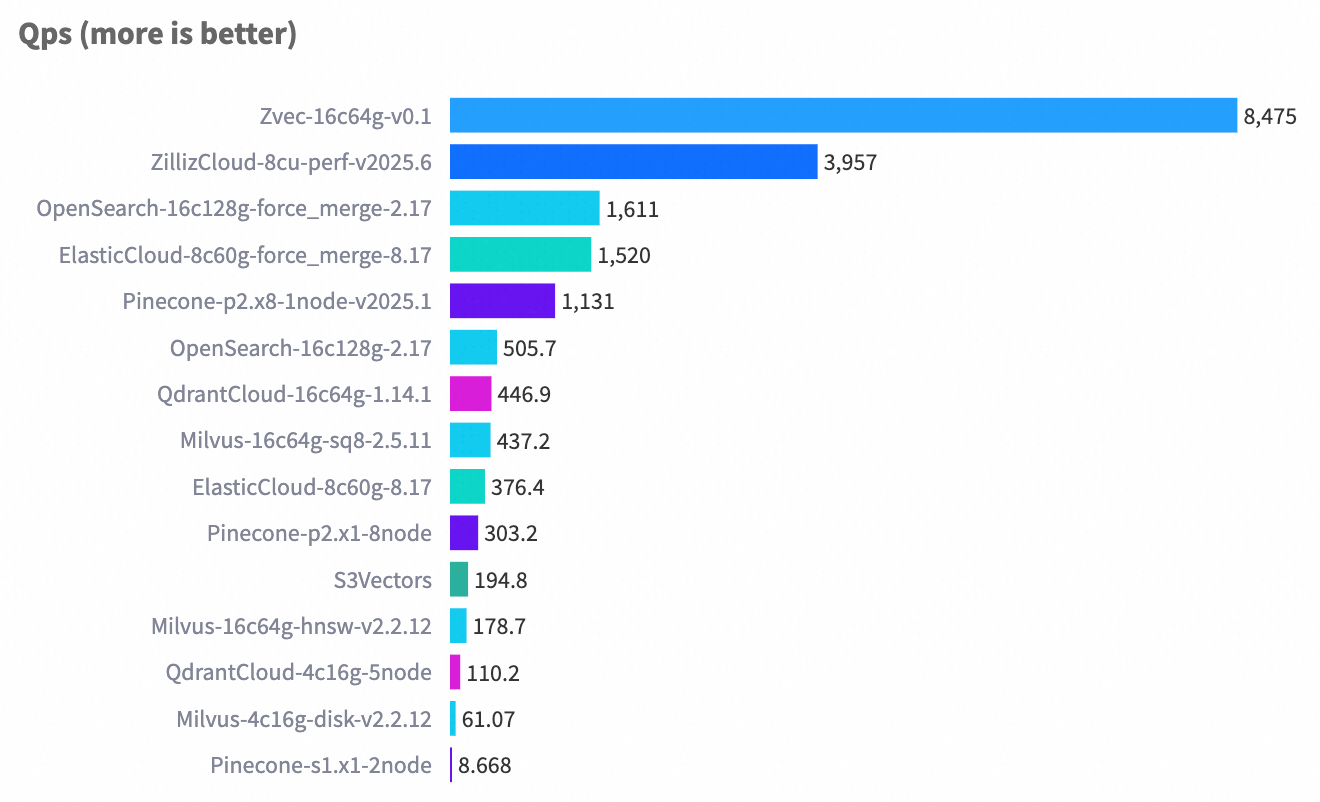
\includegraphics[width=0.92\textwidth,keepaspectratio]{images/zvec Performance at Scale.png}
    \caption{ZVec performance at scale (official benchmark overview).}
    \label{fig:zvec-performance}
\end{figure}

\textbf{Redis.} A cache layer stores reasoning traces, session context, and frequently accessed metadata so repeated analytical sessions remain responsive. Cache entries are keyed by session and query identifiers; invalidation follows session lifecycle events rather than corpus-wide flushes, so ingestion backfills do not unnecessarily evict active conversations.

\section{Retrieval and Reasoning Implementation}

The \texttt{ReasoningEngine} service implements the plan--retrieve--synthesize loop described in Chapter~3. Regardless of mode, the skeleton comprises planning (when enabled), ZVec chunk retrieval, optional Neo4j entity lookup and traversal (depth~2 by default, up to \texttt{MAX\_HOPS = 3} iterations in multi-hop modes), synthesis through Mistral with structured citation fields, and serialization of a reasoning trace for the frontend. Optional web search augments the local corpus when the query signals recency or when the user explicitly enables it.

Figure~\ref{fig:reasoning-modes-implementation} maps the three production modes to retrieval depth. \textbf{RAG mode} skips decomposition and graph expansion: the original question queries ZVec once, chunks are deduplicated, and synthesis proceeds immediately---minimizing latency for factual lookups. \textbf{Chain-of-thought mode} runs the planner, executes sub-questions sequentially, accumulates chunks and graph facts across hops, then synthesizes. \textbf{Reflexive mode} adds an audit step after each hop; insufficient evidence triggers refined retrieval before synthesis. Redis caches traces so the UI can replay steps without recomputation.

\begin{figure}[H]
    \centering
    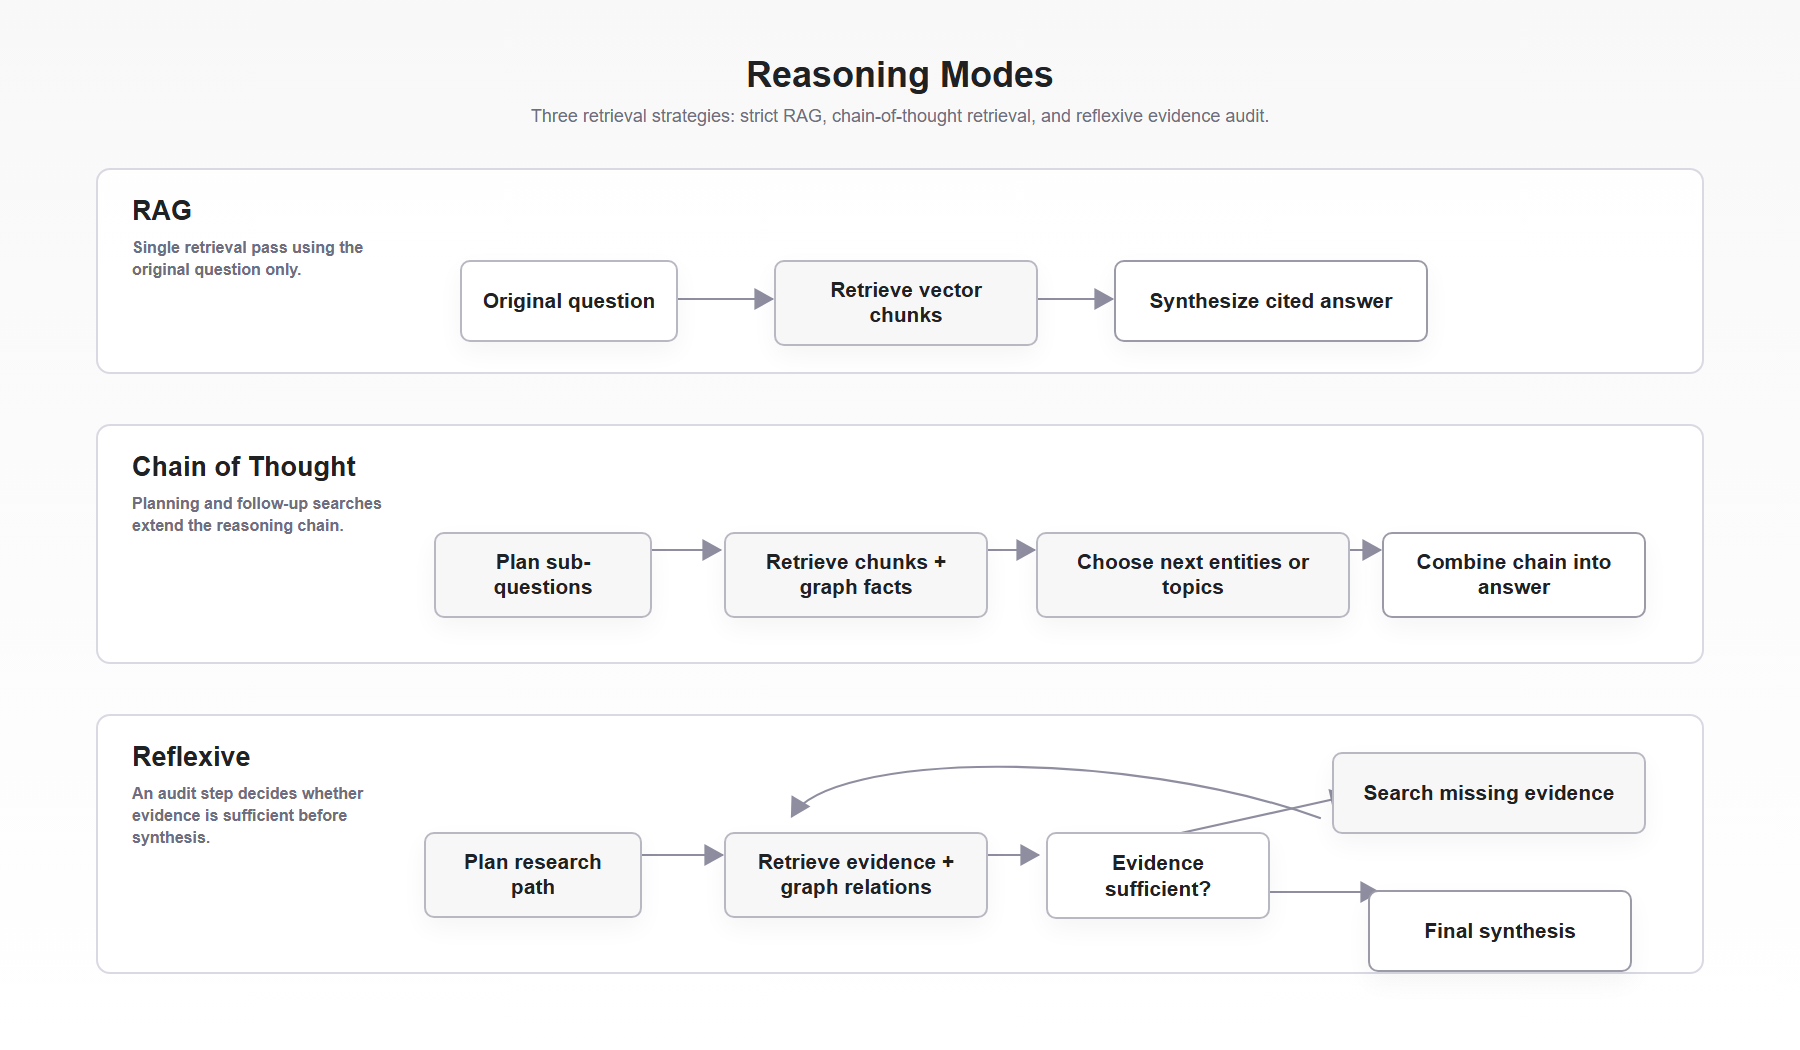
\includegraphics[width=0.96\textwidth,height=0.78\textheight,keepaspectratio]{images/reasoning_modes.png}
    \caption{Three reasoning modes in the query engine: one-hop RAG, chain-of-thought multi-hop, and reflexive control.}
    \label{fig:reasoning-modes-implementation}
\end{figure}

Hybrid ranking combines semantic scores from ZVec, graph distance to seed entities, temporal validity on edges, and deduplication of syndicated passages. Synthesis prompts require explicit source references: chunk identifiers, document titles, and graph fact summaries are passed as structured context. The FastAPI \texttt{/query} route streams thinking steps to the client using server-sent events so the chat interface can render planning, retrieval, audit, and synthesis phases in real time. Chapter~5 evaluates answer quality and grounding across modes on the same deployed endpoint.

\textbf{Optional live web search (DuckDuckGo).} All three reasoning modes can augment the local corpus with external web evidence through \texttt{DuckDuckGoSearchRun} (\texttt{services/websearch.py}). \textbf{DuckDuckGo} is a privacy-oriented search engine: it returns ranked results without user profiling and without a commercial search API key, which aligns with sovereignty constraints and with patterns used by many modern AI agents that combine indexed knowledge with fresh public web pages. The service posts queries to DuckDuckGo's HTML results endpoint (Instant Answer API as fallback), normalizes hits as \texttt{type: web\_search} objects, and passes them to synthesis separately from ZVec chunks so provenance remains explicit. The chat \textbf{Web On / Off} toggle sets \texttt{enable\_web\_search}; recency keywords can auto-enable search; administration exposes \emph{AI Search (DuckDuckGo)} for topic-driven ingestion. Figure~\ref{fig:duckduckgo-rag-websearch} summarizes the implementation flow.

\begin{figure}[H]
    \centering
    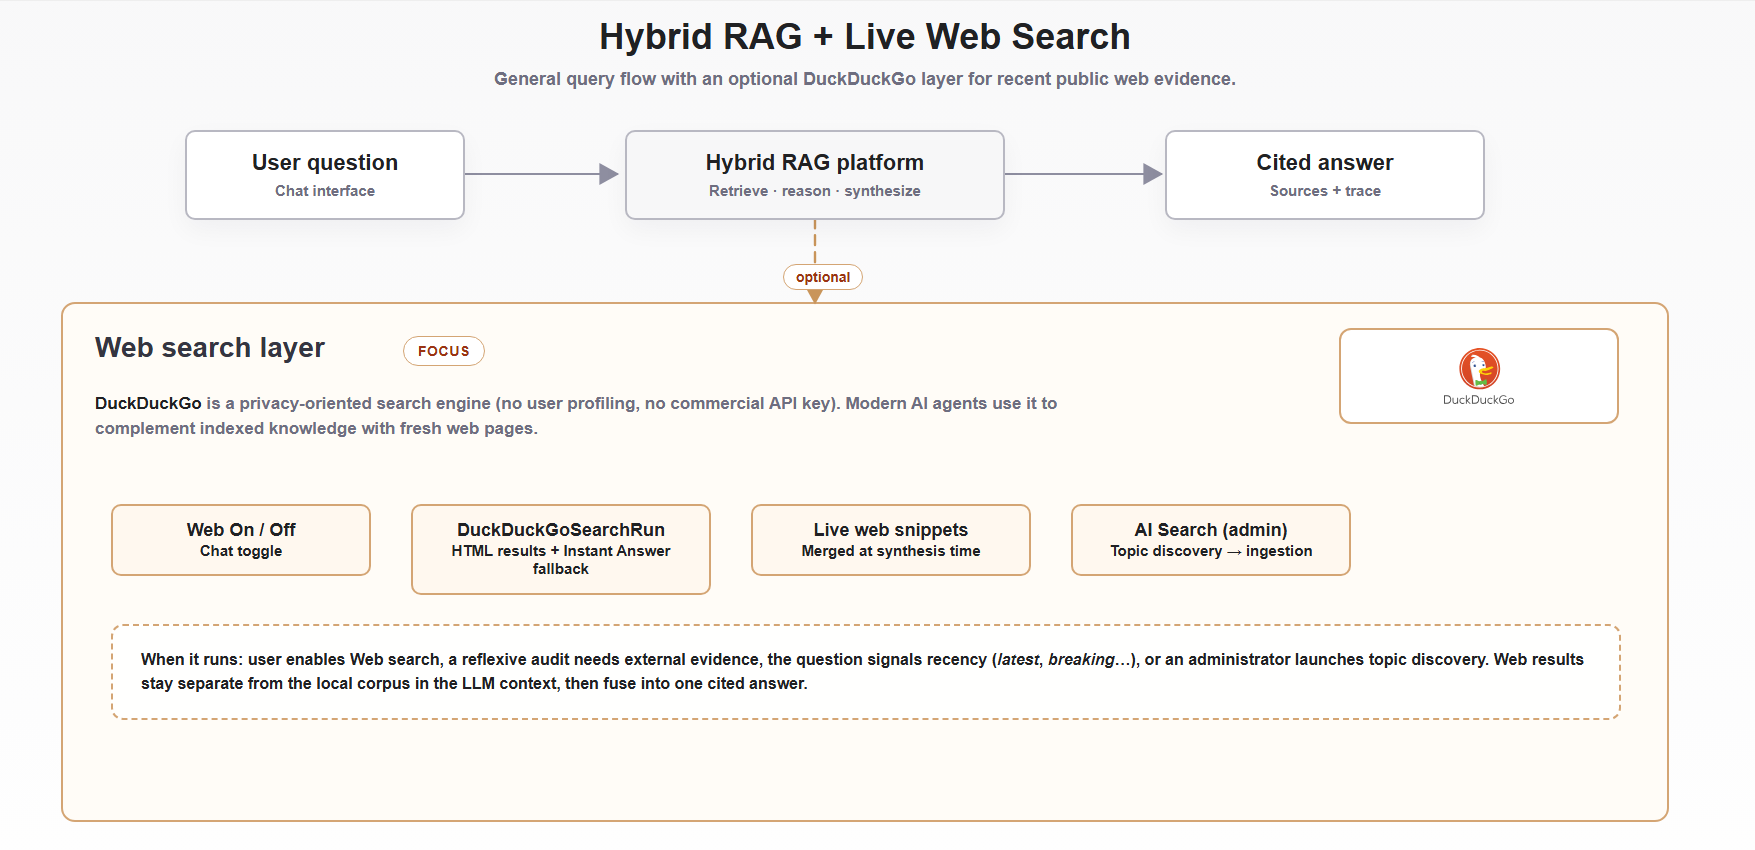
\includegraphics[width=0.96\textwidth,height=0.78\textheight,keepaspectratio]{images/duckduckgo_rag_websearch.png}
    \caption{Hybrid RAG implementation with optional DuckDuckGo web search at query time.}
    \label{fig:duckduckgo-rag-websearch}
\end{figure}

The diagram shows that internal retrieval (ZVec, Neo4j, MongoDB) remains the primary path, while DuckDuckGo supplies supplementary snippets when the user, the reflexive auditor, or an admin discovery job requires information not yet indexed locally. Web evidence does not replace the corpus; it bridges the gap until scheduled ingestion ingests the same sources permanently.

\section{Frontend Implementation}

The client is a React and Vite single-page application with React Router, TanStack Query for server state, and a resizable layout pairing a persistent chat-history sidebar with the active workspace. Routes include the home chat (\texttt{/}), session deep links (\texttt{/chat/:sessionId}), authentication (\texttt{/auth}), administration (\texttt{/admin}), graph explorer (\texttt{/graph}), legislative tracker (\texttt{/legislative/...}), political insights (\texttt{/insights/...}), and document library (\texttt{/documents}). A centralized API client wraps FastAPI endpoints for queries (including SSE streams), graph search, documents, auth, and admin operations, preserving a strict boundary between presentation and backend reasoning services.

\textbf{Analytical workspace: chat and reasoning trace.} The chat interface is the primary entry point for cited questioning. Figure~\ref{fig:ui-chat-interface} shows the layout: session sidebar, message thread, reasoning-mode selector (\texttt{rag}, \texttt{cot}, \texttt{reflexive}), and a \textbf{Web On / Web Off} control linked to DuckDuckGo retrieval in the reasoning implementation above. The mode and web flags are forwarded to the backend as \texttt{reasoning\_mode} and \texttt{enable\_web\_search}.

\begin{figure}[H]
    \centering
    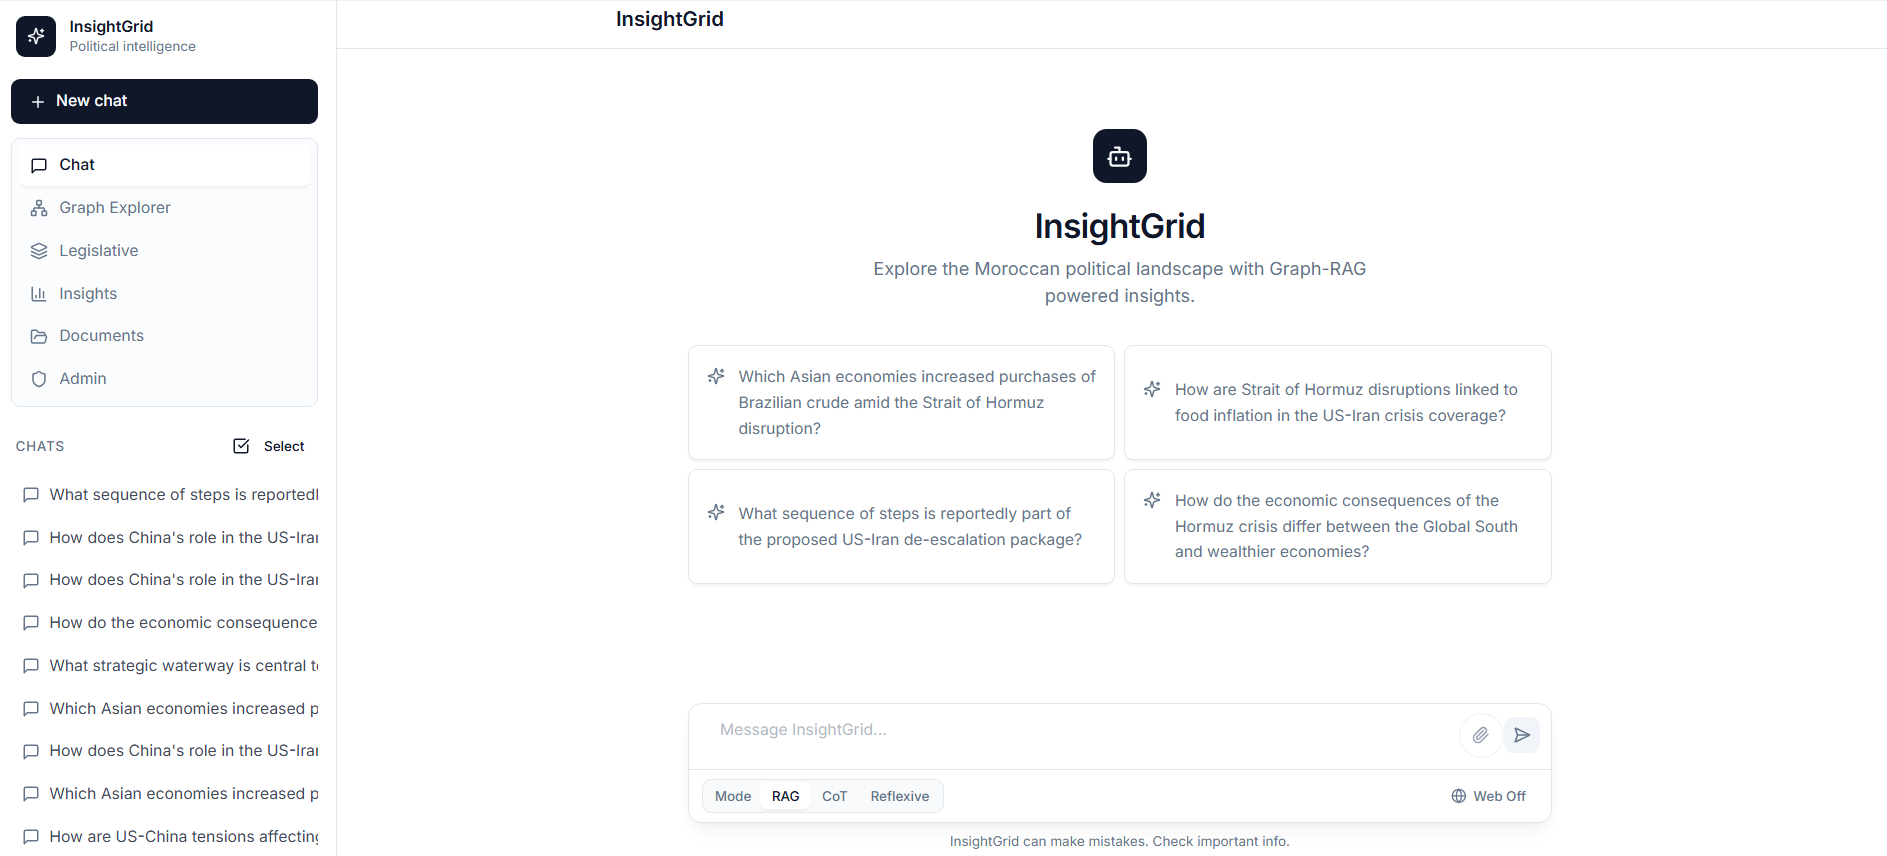
\includegraphics[width=0.96\textwidth,height=0.72\textheight,keepaspectratio]{chat interface.png}
    \caption{Chat workspace with session history sidebar and reasoning-mode controls.}
    \label{fig:ui-chat-interface}
\end{figure}

Figure~\ref{fig:ui-chat-rag} illustrates a completed answer in RAG mode: the assistant message includes inline citations, source cards, and confidence cues tied to retrieved chunks. Figure~\ref{fig:ui-chat-rag-trace} expands the reasoning trace panel, exposing sequential steps (ZVec retrieval, synthesis) so the user can verify which evidence supported each claim---implementing FR-07 at interface level.

\begin{figure}[H]
    \centering
    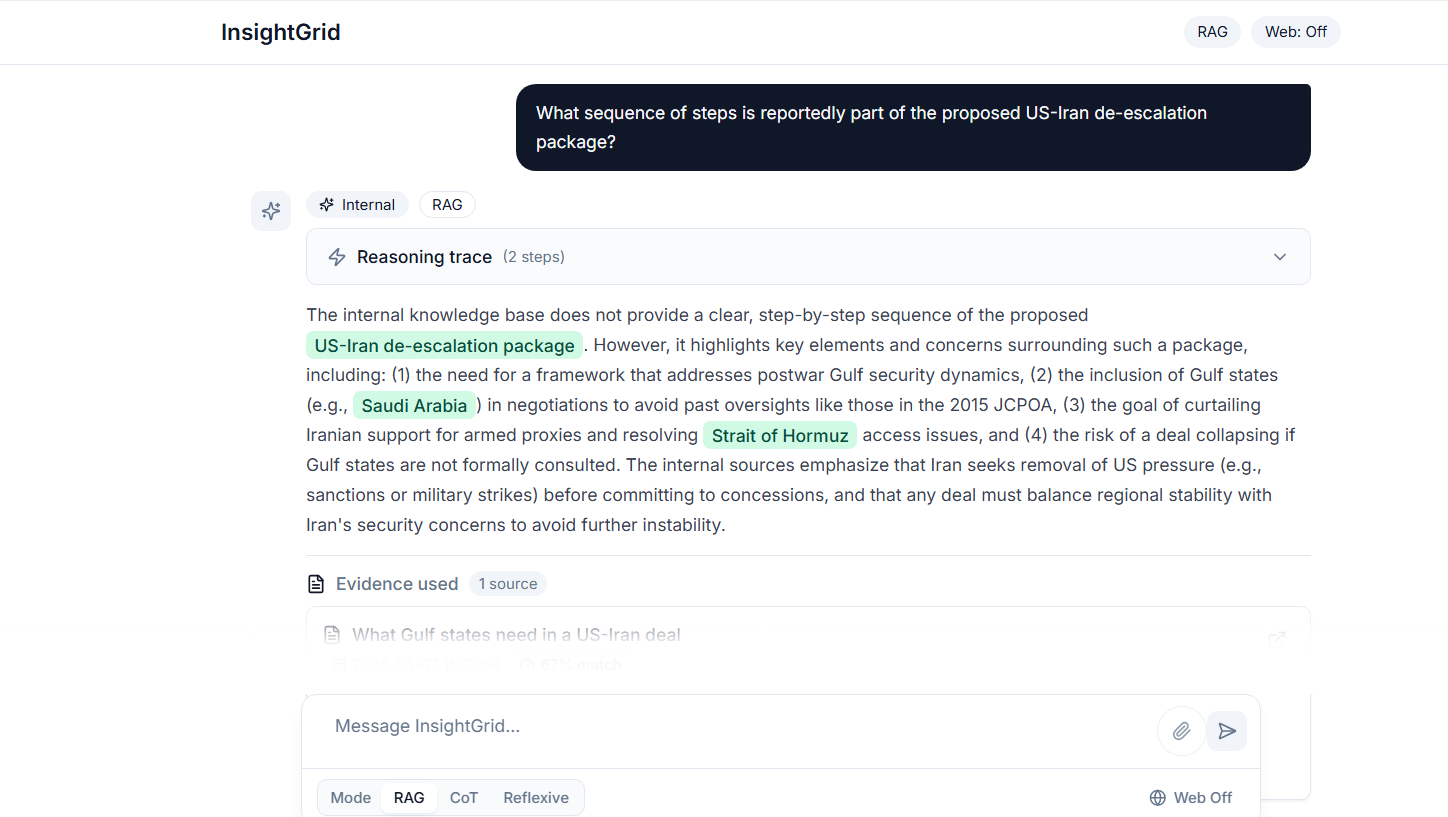
\includegraphics[width=0.96\textwidth,height=0.72\textheight,keepaspectratio]{chat question rag mode.png}
    \caption{Cited answer produced in standard RAG mode with linked source evidence.}
    \label{fig:ui-chat-rag}
\end{figure}

\begin{figure}[H]
    \centering
    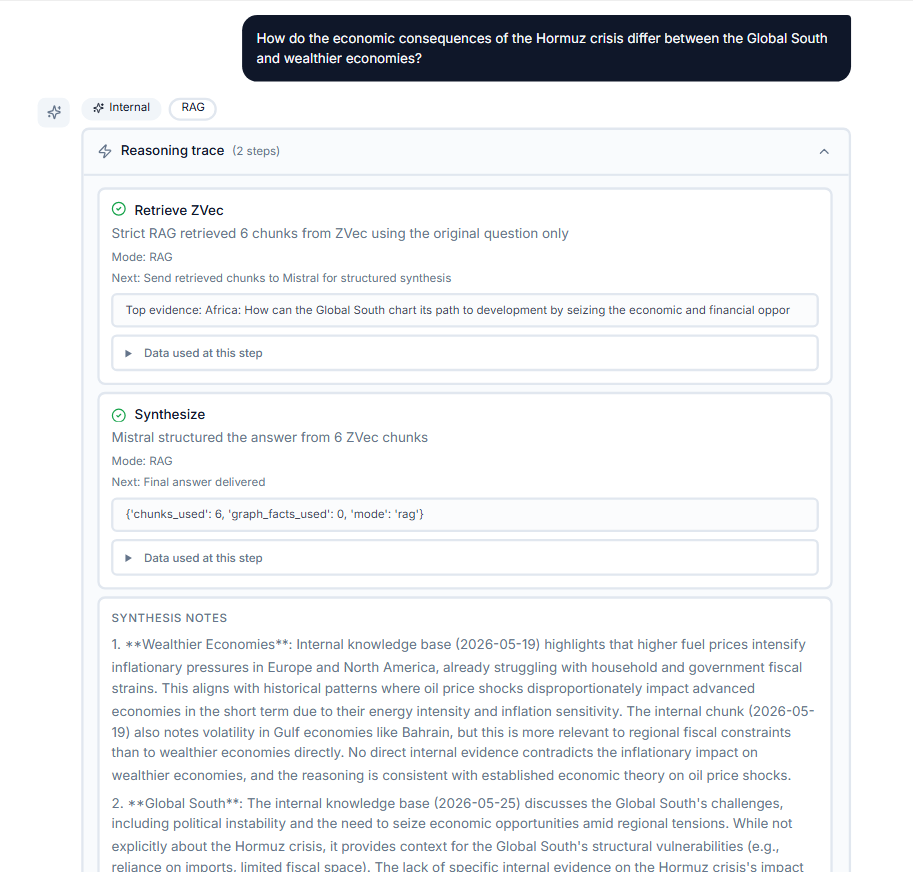
\includegraphics[width=0.96\textwidth,height=0.72\textheight,keepaspectratio]{chat question rag mode reasnoing trace.png}
    \caption{Expandable reasoning trace for a RAG-mode query (retrieval and synthesis steps).}
    \label{fig:ui-chat-rag-trace}
\end{figure}

\textbf{Document library and graph explorer.} The document library (Figure~\ref{fig:ui-documents}) lists ingested sources with filters on metadata, supporting the use case in which analysts verify wording and provenance before trusting synthesized summaries. Selecting a document opens normalized text and extraction status without leaving the analytical shell.

\begin{figure}[H]
    \centering
    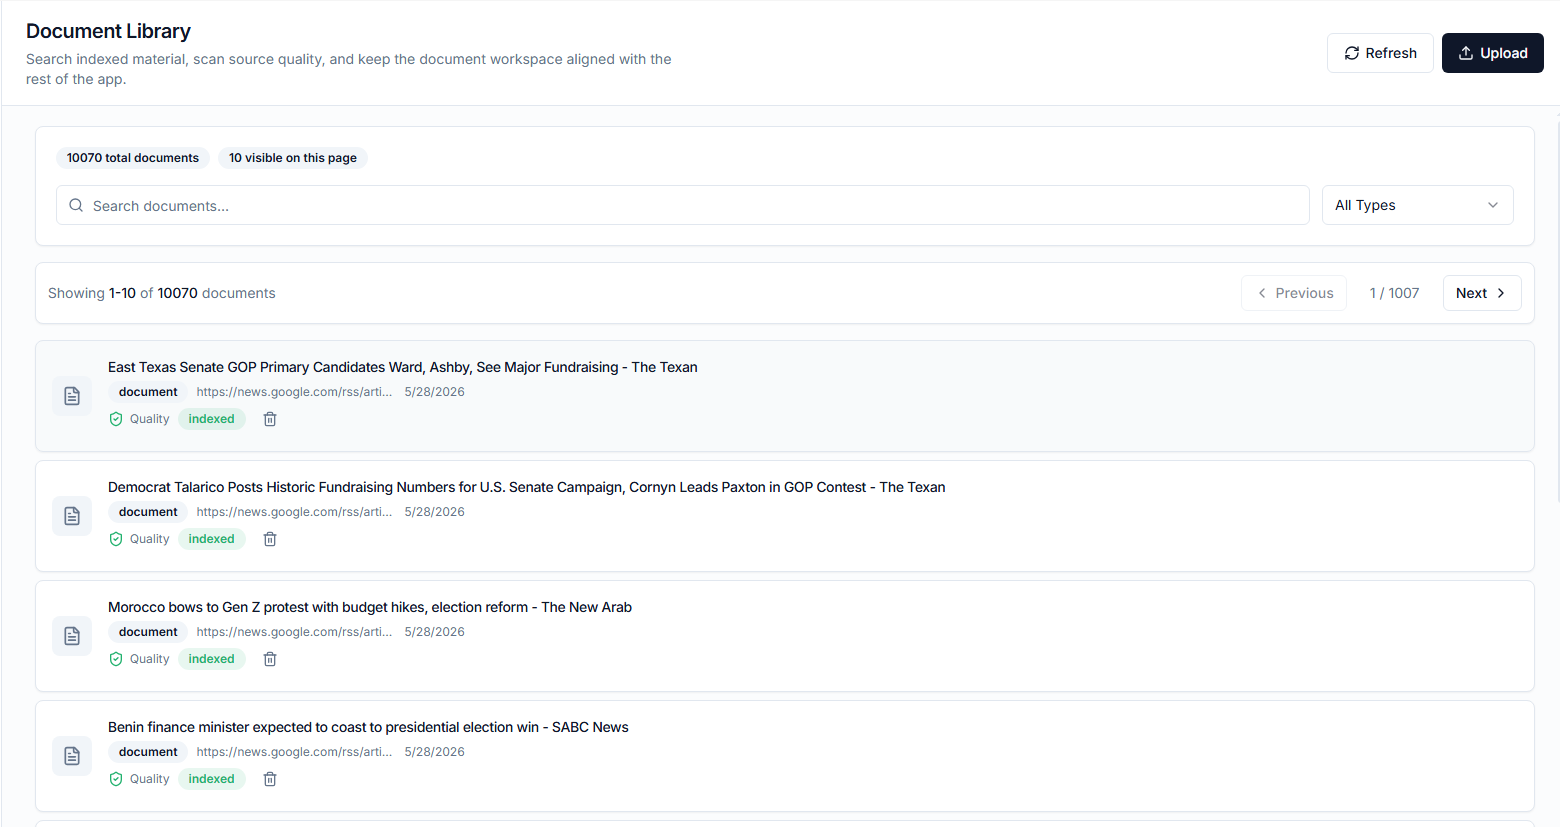
\includegraphics[width=0.96\textwidth,height=0.72\textheight,keepaspectratio]{page documents library.png}
    \caption{Document library for inspecting ingested corpus items and metadata.}
    \label{fig:ui-documents}
\end{figure}

The graph explorer (Figure~\ref{fig:ui-graph}) renders force-directed neighborhoods with \texttt{react-force-graph-2d} and D3.js interactions: pan, zoom, node selection, and typed edge labels. Users pivot from a chat answer to structural exploration by opening the same entities in the graph view, closing the loop between conversational synthesis and relational inspection.

\begin{figure}[H]
    \centering
    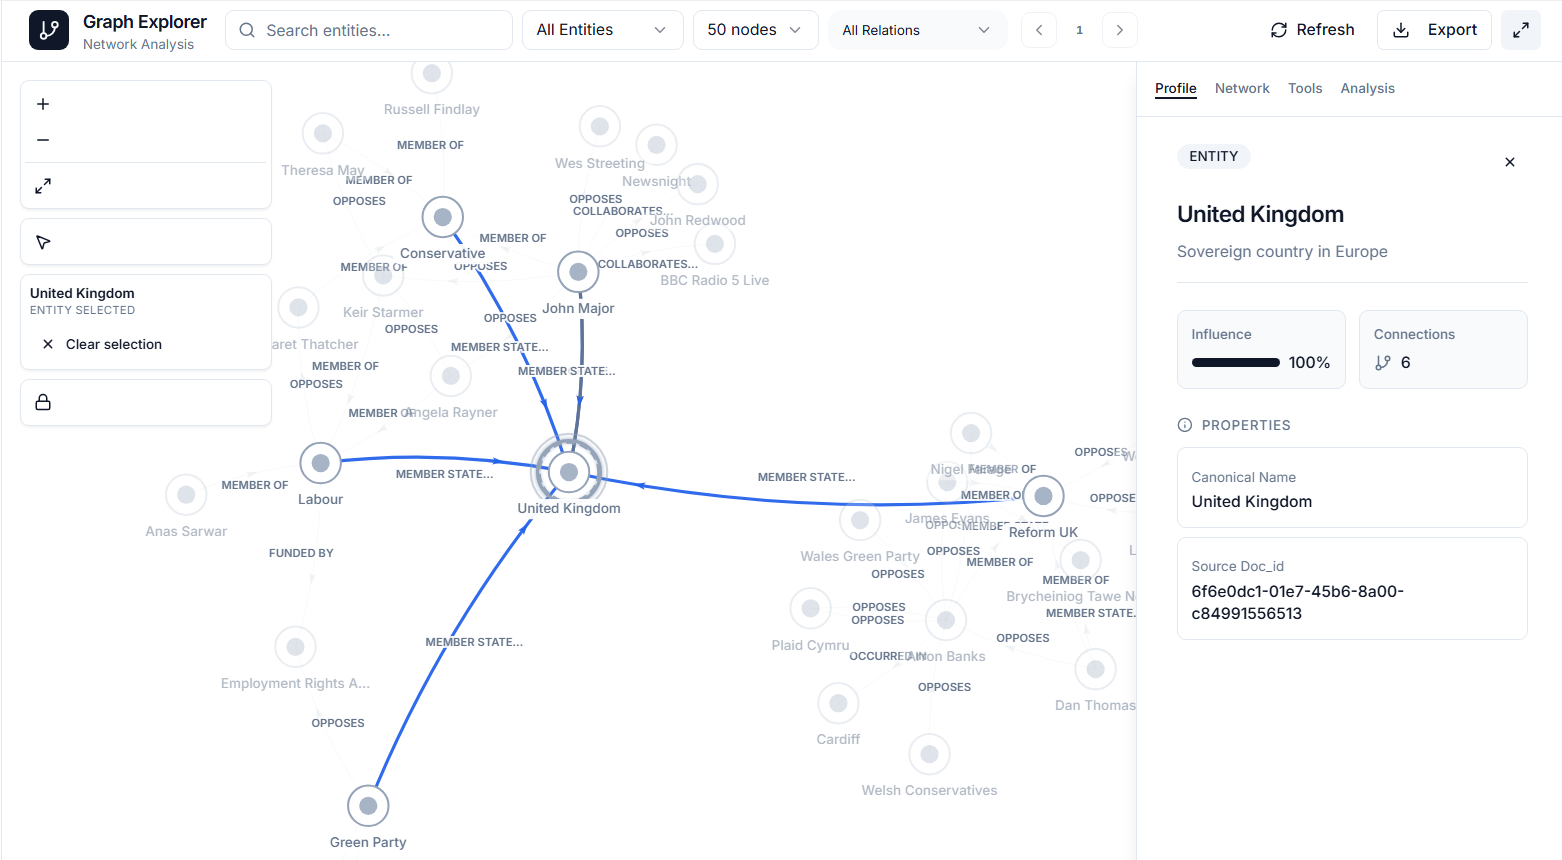
\includegraphics[width=0.96\textwidth,height=0.72\textheight,keepaspectratio]{page graph explorer.png}
    \caption{Graph explorer with interactive entity neighborhood layout.}
    \label{fig:ui-graph}
\end{figure}

\textbf{Legislative and structured political views.} The legislative tracker exposes MongoDB structured records extracted from policy corpora. Figure~\ref{fig:ui-legislative-bills} presents bill listings with status and sponsorship metadata; Figure~\ref{fig:ui-legislative-votes} focuses on roll-call votes; Figure~\ref{fig:ui-legislative-committees} shows committee assignments and related actors. These views complement graph traversal by offering tabular, schema-stable summaries for institutional monitoring.

\begin{figure}[H]
    \centering
    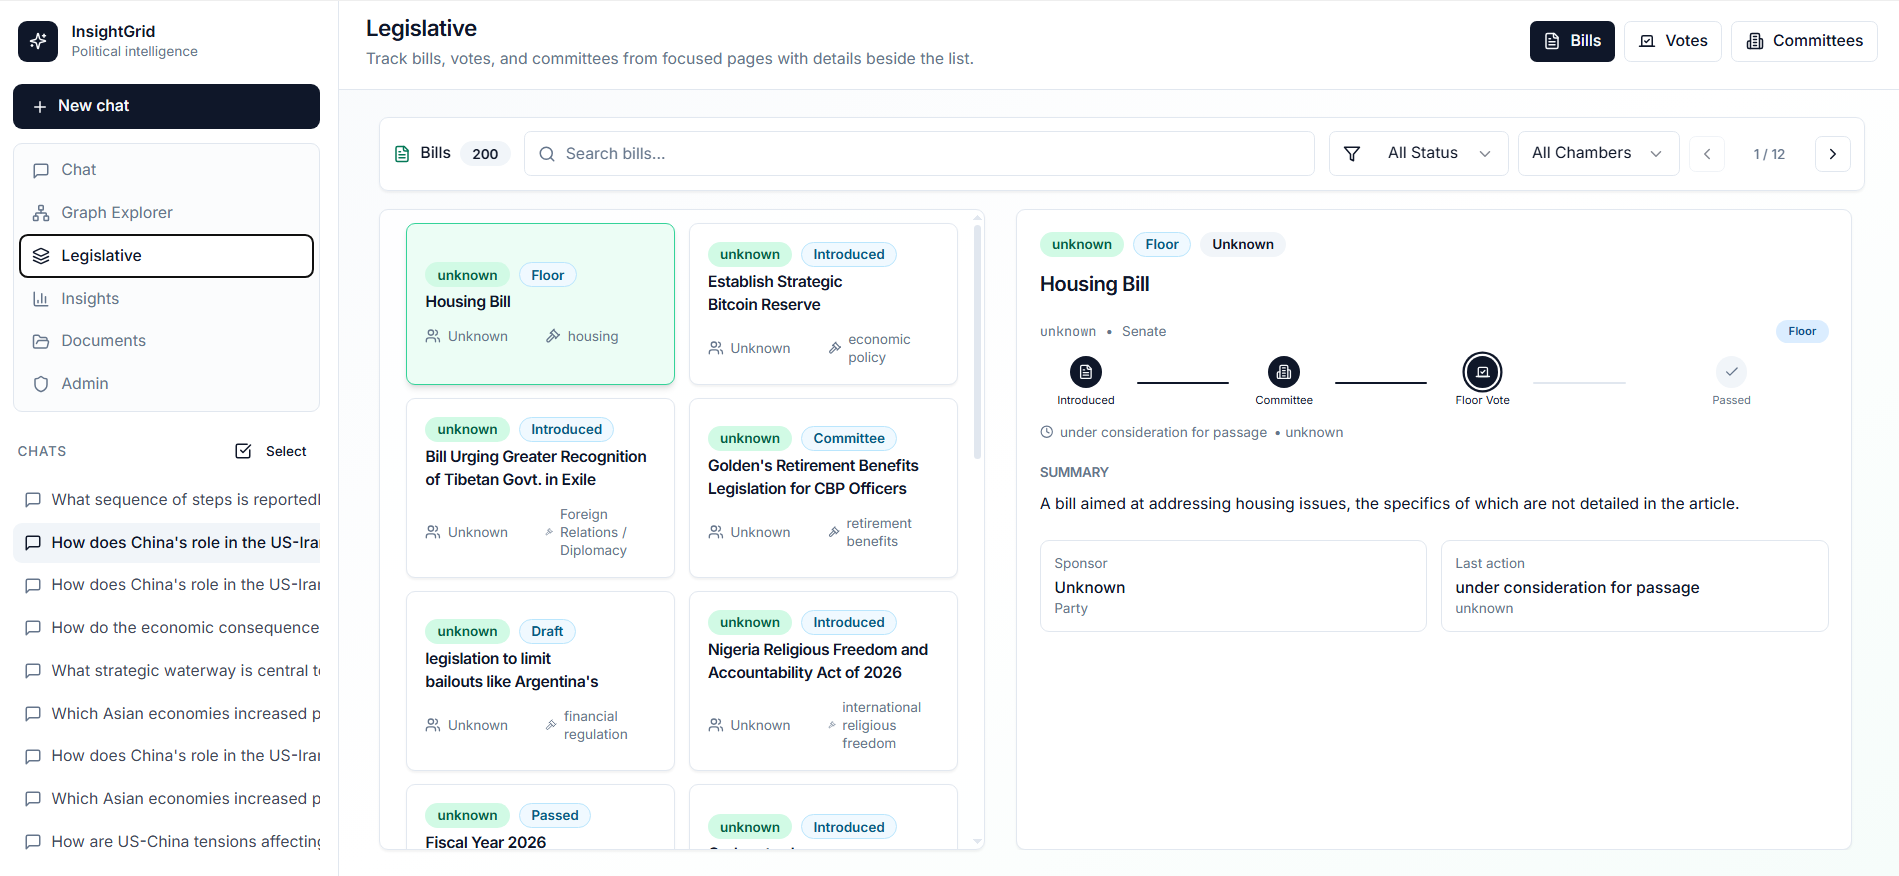
\includegraphics[width=0.96\textwidth,height=0.72\textheight,keepaspectratio]{page legislative bills.png}
    \caption{Legislative tracker: bills view with structured metadata from extracted records.}
    \label{fig:ui-legislative-bills}
\end{figure}

\begin{figure}[H]
    \centering
    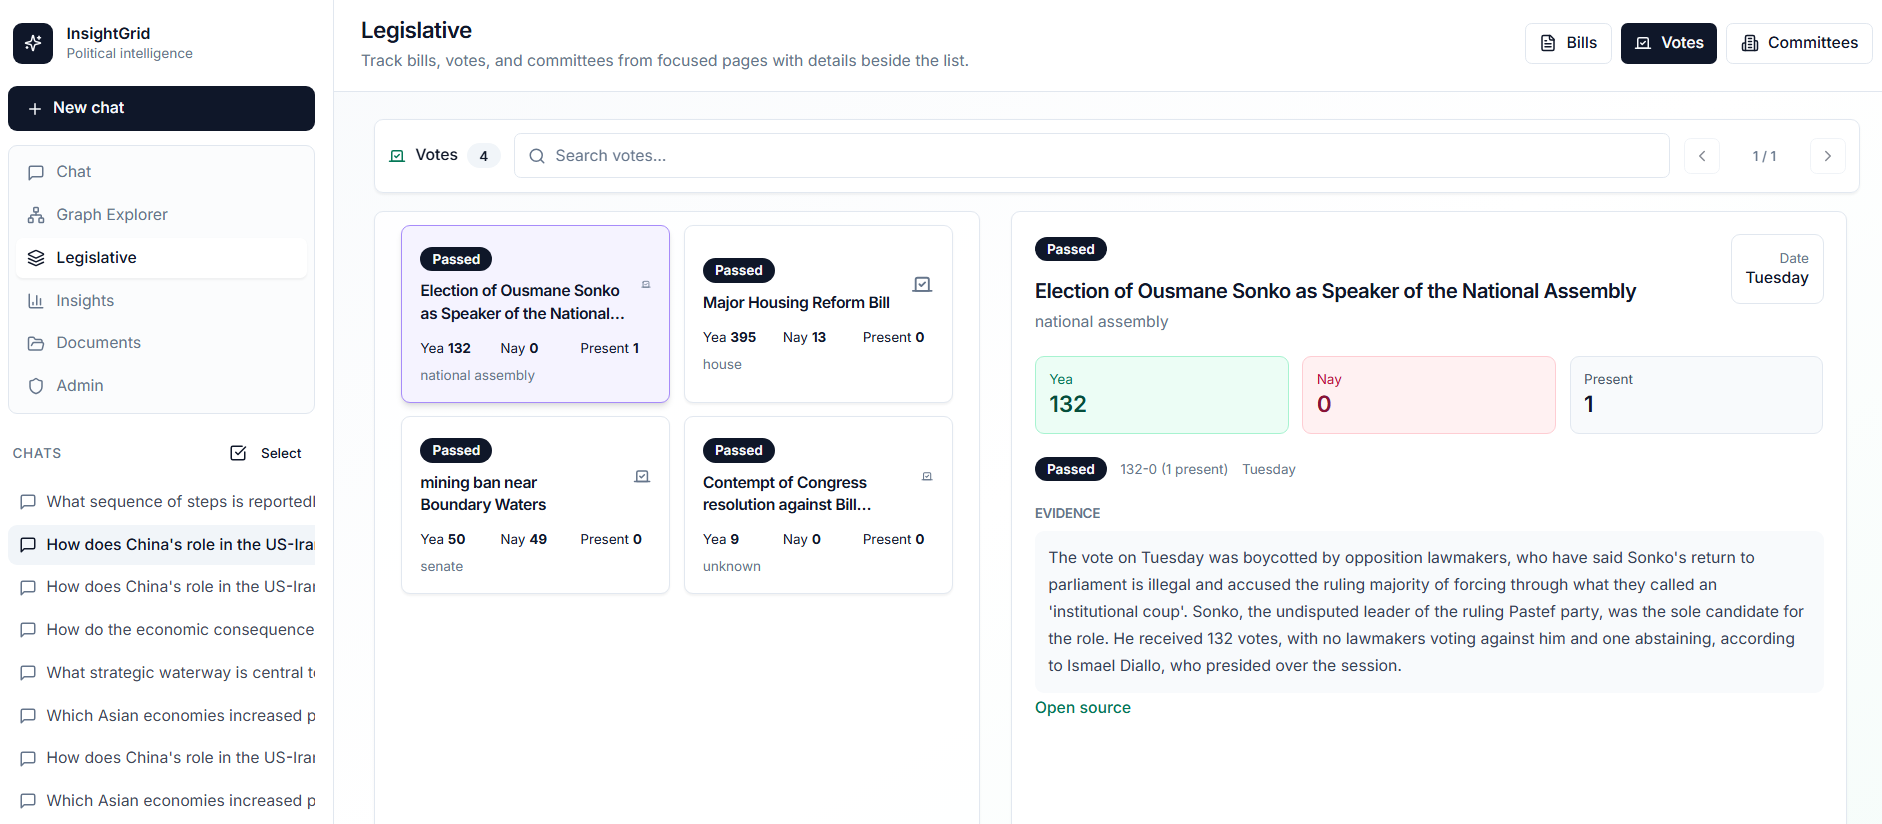
\includegraphics[width=0.96\textwidth,height=0.72\textheight,keepaspectratio]{page legislative Votes.png}
    \caption{Legislative tracker: votes view linking legislators to roll-call outcomes.}
    \label{fig:ui-legislative-votes}
\end{figure}

\begin{figure}[H]
    \centering
    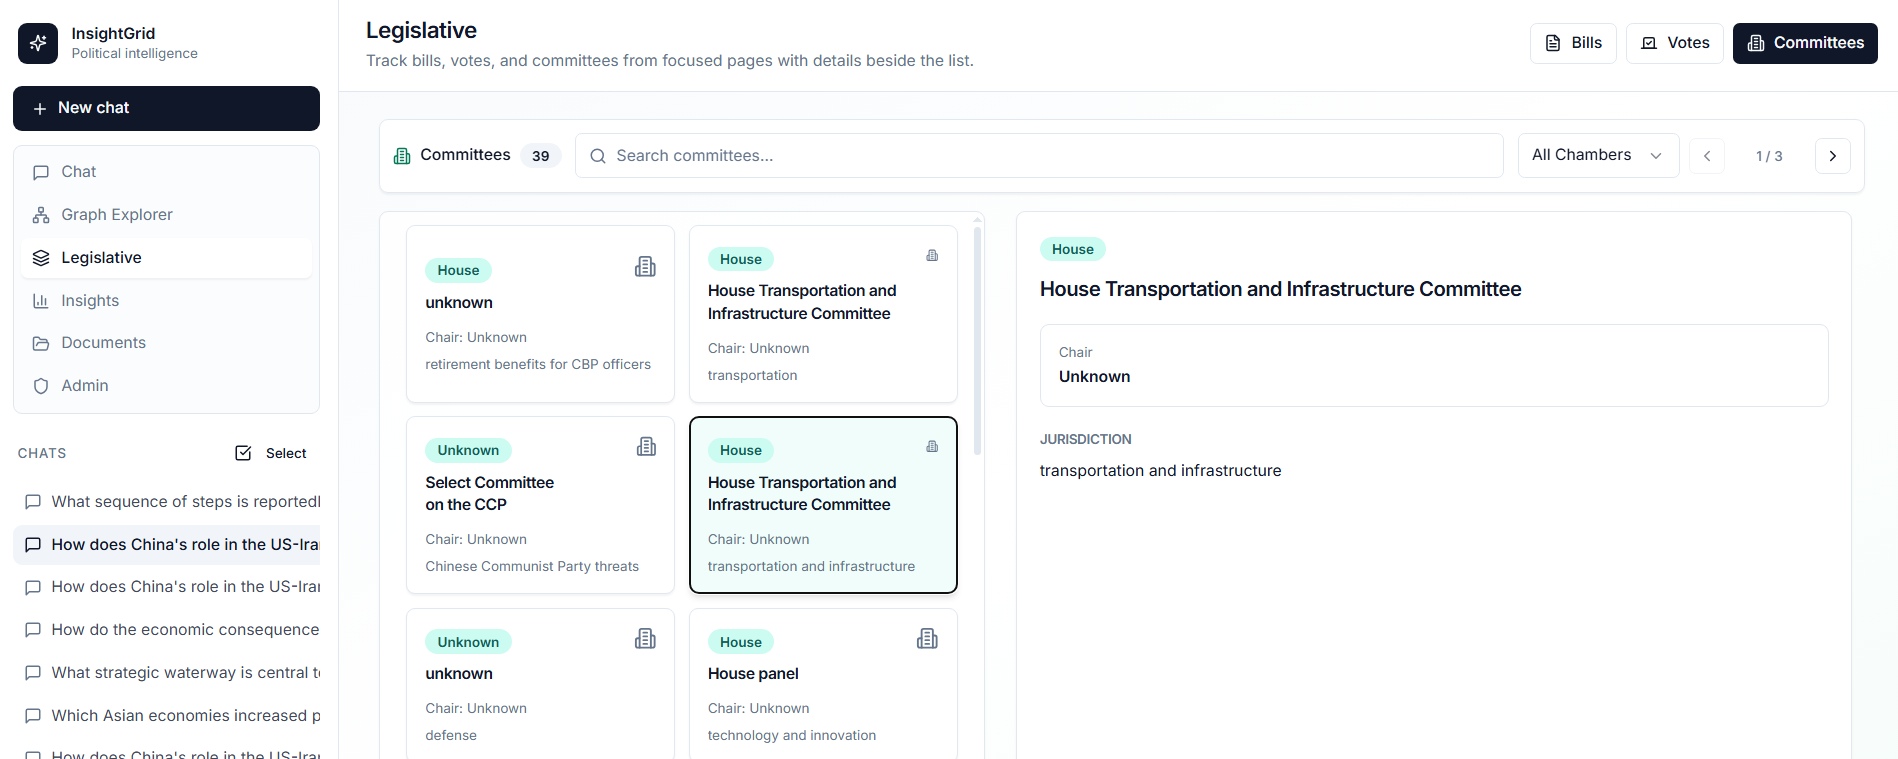
\includegraphics[width=0.96\textwidth,height=0.72\textheight,keepaspectratio]{page legislative committes.png}
    \caption{Legislative tracker: committees view for institutional roles and memberships.}
    \label{fig:ui-legislative-committees}
\end{figure}

\textbf{Political insights dashboards.} The \texttt{/insights/...} module groups four analytical tabs on top of MongoDB structured records, Neo4j neighborhoods, and derived analytics services.

The \textbf{finance} tab (Figure~\ref{fig:ui-insights-finance}) queries campaign-contribution and donor records filtered by electoral cycle, country, entity type, and free-text search. It surfaces top donors, aggregated amounts, and finance-related conflict flags when the same actor appears on both sides of a funding relationship---supporting scrutiny of economic influence without leaving the platform.

The \textbf{trends} tab (Figure~\ref{fig:ui-insights-trends}) plots mention frequency and sentiment volatility for entities or topics over selectable windows (e.g.\ seven days) and optional regional filters. Recharts time-series views help analysts distinguish sustained narrative shifts from short-lived spikes in media coverage.

The \textbf{conflicts} tab (Figure~\ref{fig:ui-insights-conflicts}) lists \texttt{conflict\_flags} extracted from documents: opposing stances, shared donors with competing beneficiaries, committee overlaps, and similar patterns where two actors occupy incompatible roles in the evidence. Each row links back to document provenance for manual verification.

The \textbf{compare} tab implements pairwise entity intelligence across eight analytical aspects (or all aspects at once). The user selects two canonical entities via autocomplete (\texttt{/graph/search} suggestions), then chooses an \emph{aspect scope}:
\begin{itemize}[leftmargin=*, itemsep=2pt]
\item \textbf{Political stance} --- party alignment, ideology, support/opposition, coalitions, elections;
\item \textbf{Economic policy} --- budgets, taxation, trade, inflation, subsidies, public spending;
\item \textbf{Influence and network} --- allies, donors, committees, appointments, lobbying ties;
\item \textbf{Governance style} --- reform, transparency, accountability, institutional oversight;
\item \textbf{Legislative record} --- bills, amendments, roll-call votes, committee hearings;
\item \textbf{Foreign policy} --- diplomacy, alliances, sanctions, security treaties;
\item \textbf{Public sentiment} --- polls, approval, protests, media backlash, popularity;
\item \textbf{Risk and conflict exposure} --- scandals, investigations, lawsuits, controversies;
\item \textbf{All aspects} --- runs the full matrix below in one report.
\end{itemize}

Figure~\ref{fig:ui-insights-compare-01} shows the selection panel (two entities + aspect dropdown). The backend (\texttt{POST /political/compare}) resolves both subjects in Neo4j, fetches ZVec/MongoDB evidence filtered by aspect keywords, computes shortest-path graph distance, and builds an \textbf{aspect matrix} (Figure~\ref{fig:ui-insights-compare-02}): for each row, evidence scores for entity~A, entity~B, term overlap, shared neighbors, and graph proximity. Cells summarize how strongly each actor is documented on that dimension.

Figure~\ref{fig:ui-insights-compare-03} presents the narrative layer: \emph{convergences} (shared terms, common neighbors, short graph paths), \emph{divergences} (unique evidence terms and asymmetric neighborhoods), an LLM-generated \emph{conclusion}, and optional \emph{graph path} visualization between the two nodes. The report can be exported as JSON for offline review. This three-step flow---configure, matrix, interpret---mirrors analyst practice: quantify overlap on defined dimensions before drawing qualitative judgments.

\begin{figure}[H]
    \centering
    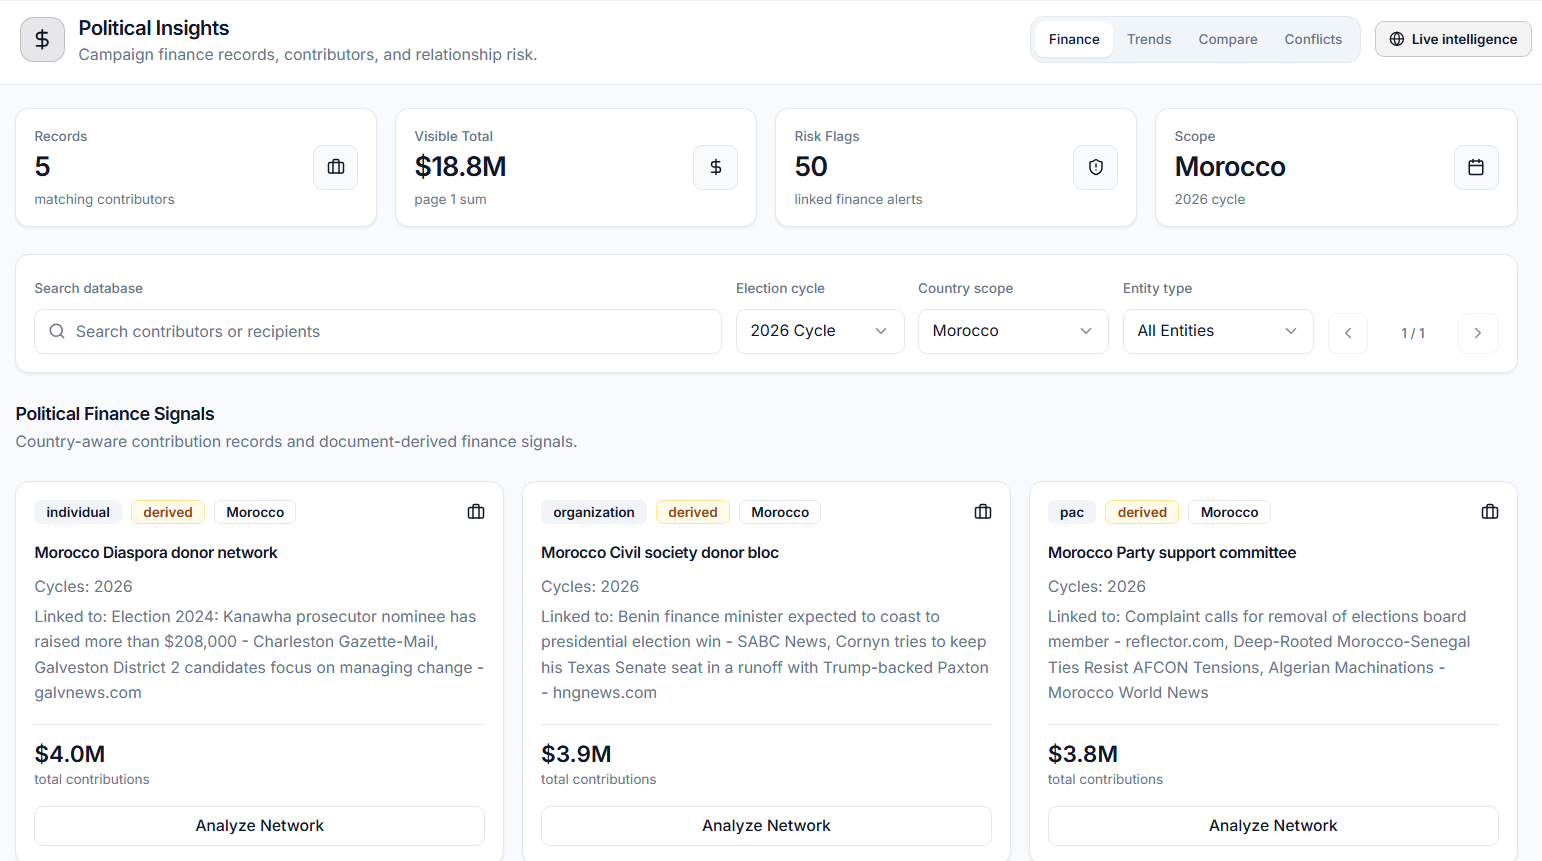
\includegraphics[width=0.96\textwidth,height=0.72\textheight,keepaspectratio]{page insights finance.png}
    \caption{Political insights: campaign finance dashboard.}
    \label{fig:ui-insights-finance}
\end{figure}

\begin{figure}[H]
    \centering
    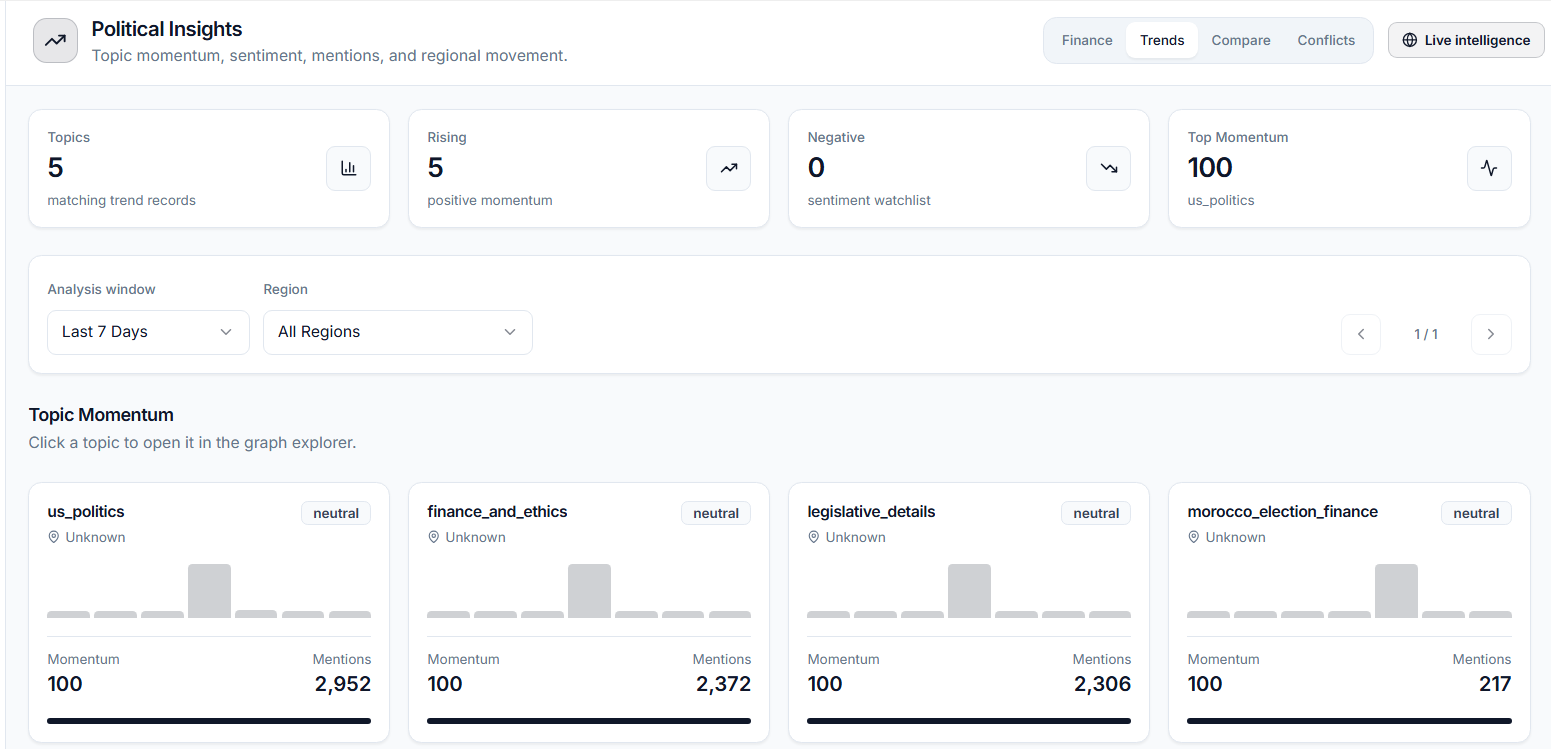
\includegraphics[width=0.96\textwidth,height=0.72\textheight,keepaspectratio]{page insights trends.png}
    \caption{Political insights: temporal trend tracking for entities or topics.}
    \label{fig:ui-insights-trends}
\end{figure}

\begin{figure}[H]
    \centering
    
\includegraphics[width=0.96\textwidth,height=0.72\textheight,keepaspectratio]{page insights compare 01.png}
    \caption{Entity comparison workflow (step 1): selection of actors or topics to compare.}
    \label{fig:ui-insights-compare-01}
\end{figure}

\begin{figure}[H]
    \centering
    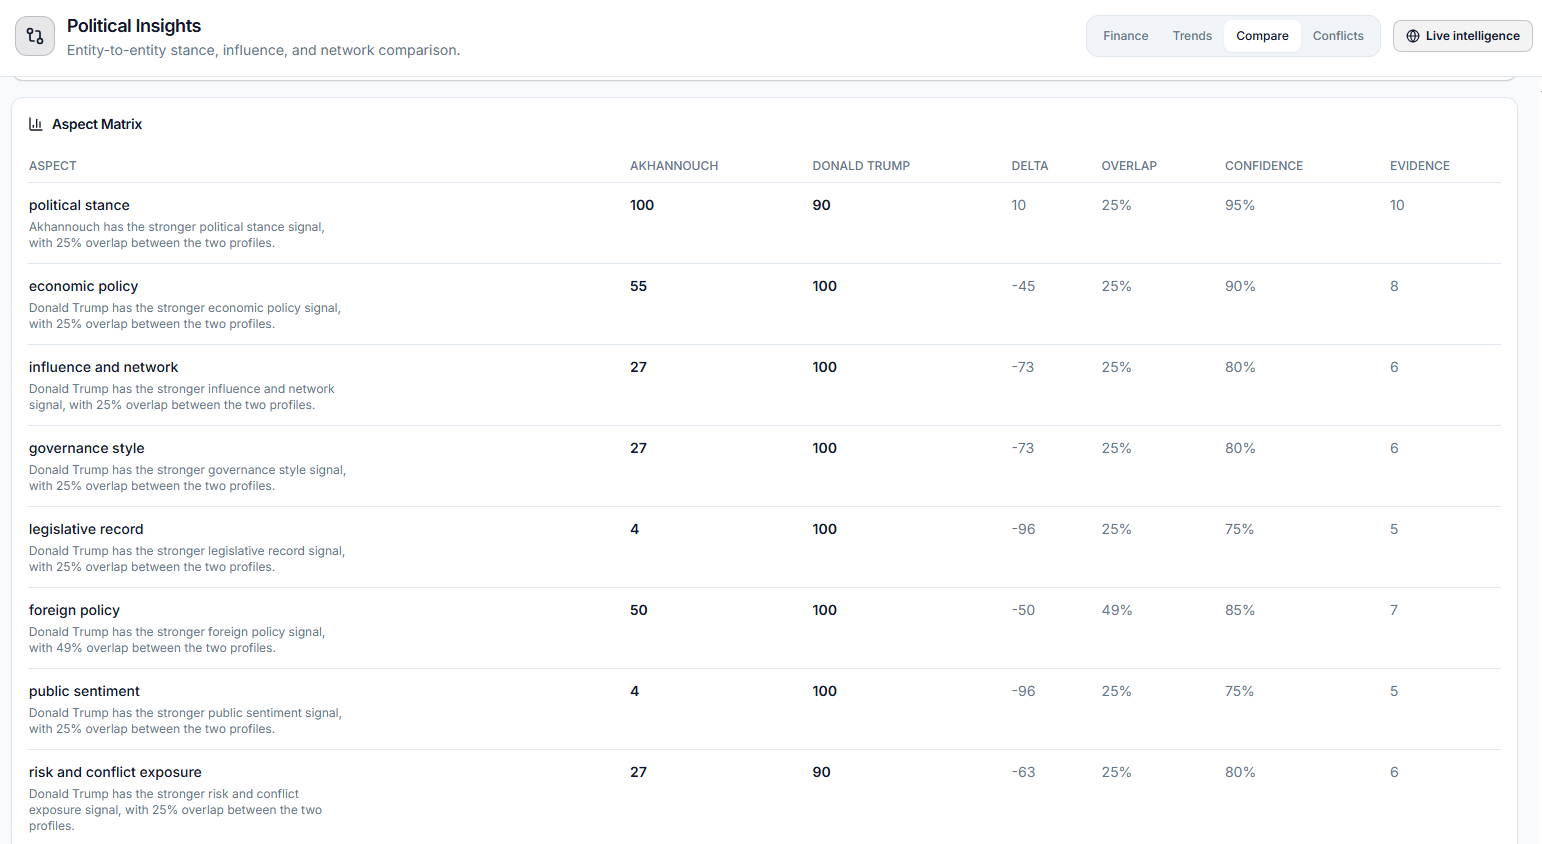
\includegraphics[width=0.96\textwidth,height=0.72\textheight,keepaspectratio]{page insights compare 02 matrix.png}
    \caption{Entity comparison workflow (step 2): relation matrix between selected entities.}
    \label{fig:ui-insights-compare-02}
\end{figure}

\begin{figure}[H]
    \centering
    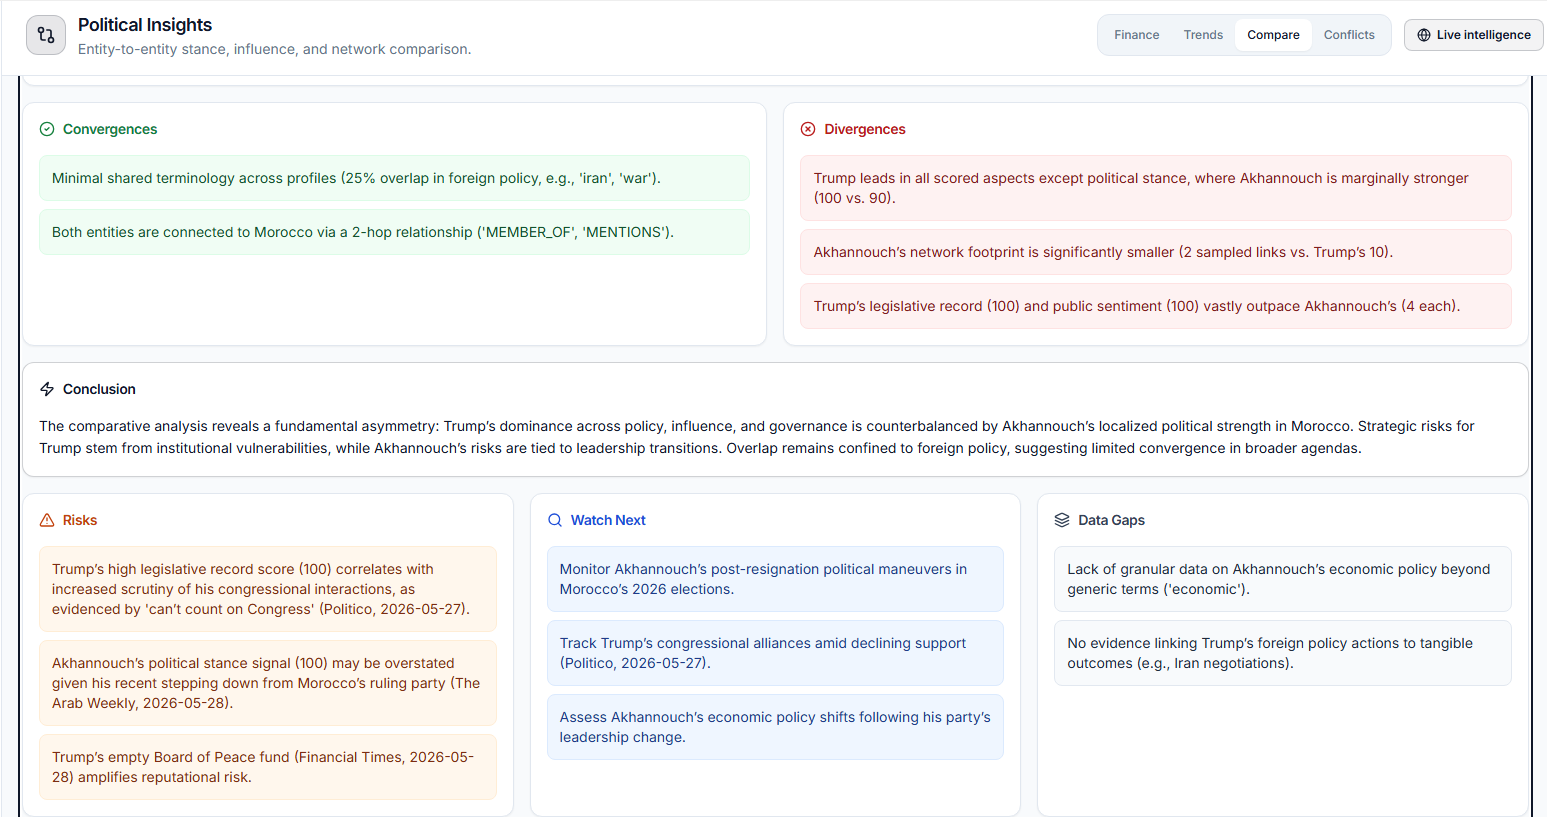
\includegraphics[width=0.96\textwidth,height=0.72\textheight,keepaspectratio]{page insights compare 03 conv div conclusion.png}
    \caption{Entity comparison workflow (step 3): convergence, divergence, and narrative conclusion.}
    \label{fig:ui-insights-compare-03}
\end{figure}

\begin{figure}[H]
    \centering
    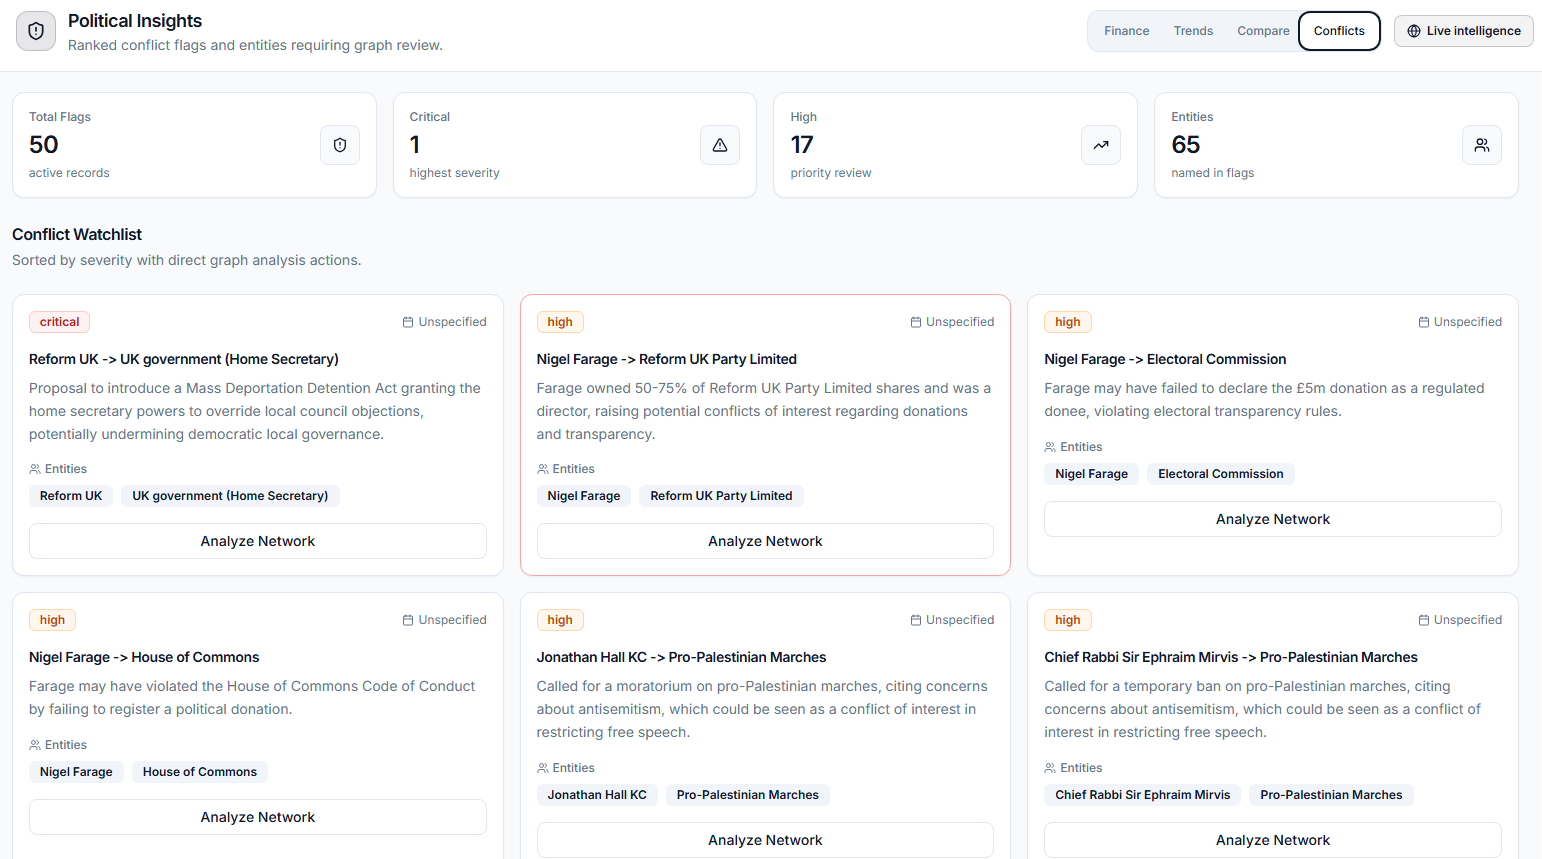
\includegraphics[width=0.96\textwidth,height=0.72\textheight,keepaspectratio]{page insights conflicts.png}
    \caption{Political insights: conflict and opposing-stance visualization.}
    \label{fig:ui-insights-conflicts}
\end{figure}

\textbf{Administration dashboard.} Administrative screens implement supervised ingestion (Chapter~2). Figure~\ref{fig:ui-admin-dashboard} summarizes service health, corpus counts, graph statistics, and recent activity. Figure~\ref{fig:ui-admin-scraped} controls import of scraped JSON batches into MongoDB and backfill into ZVec. Figure~\ref{fig:ui-admin-cron} exposes cron scheduler configuration and agentic trend-collection jobs. Figure~\ref{fig:ui-admin-topic} provides advanced topic search: administrators enter thematic queries that trigger DuckDuckGo-backed discovery (\emph{AI Search}), after which selected URLs follow the standard scrape--normalize--extract pipeline. Together these panels form the operational cockpit of the autonomous crawler rather than a passive monitoring page.

\begin{figure}[H]
    \centering
    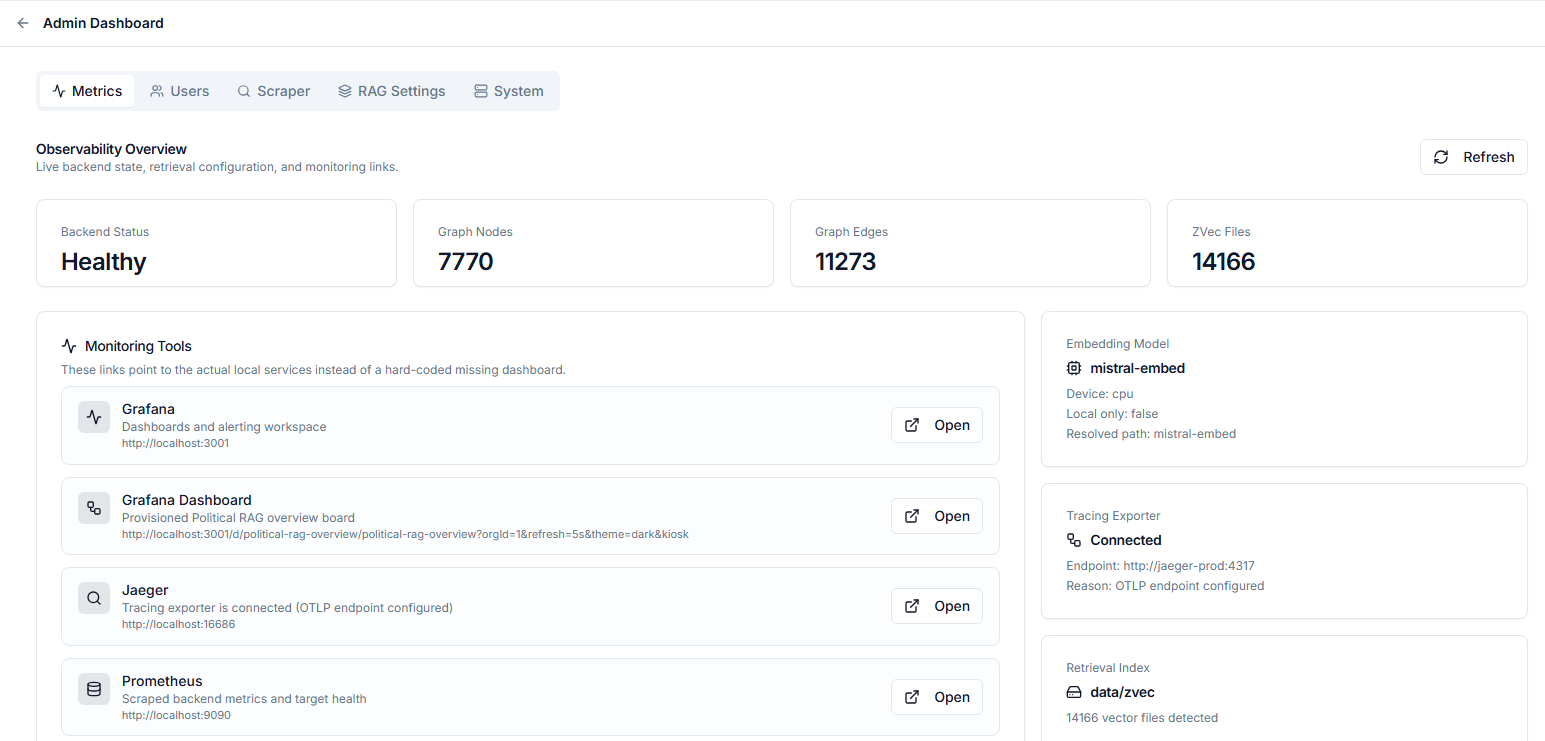
\includegraphics[width=0.96\textwidth,height=0.72\textheight,keepaspectratio]{page admin dashboard.png}
    \caption{Administration dashboard: health metrics, corpus counts, and pipeline overview.}
    \label{fig:ui-admin-dashboard}
\end{figure}

\begin{figure}[H]
    \centering
    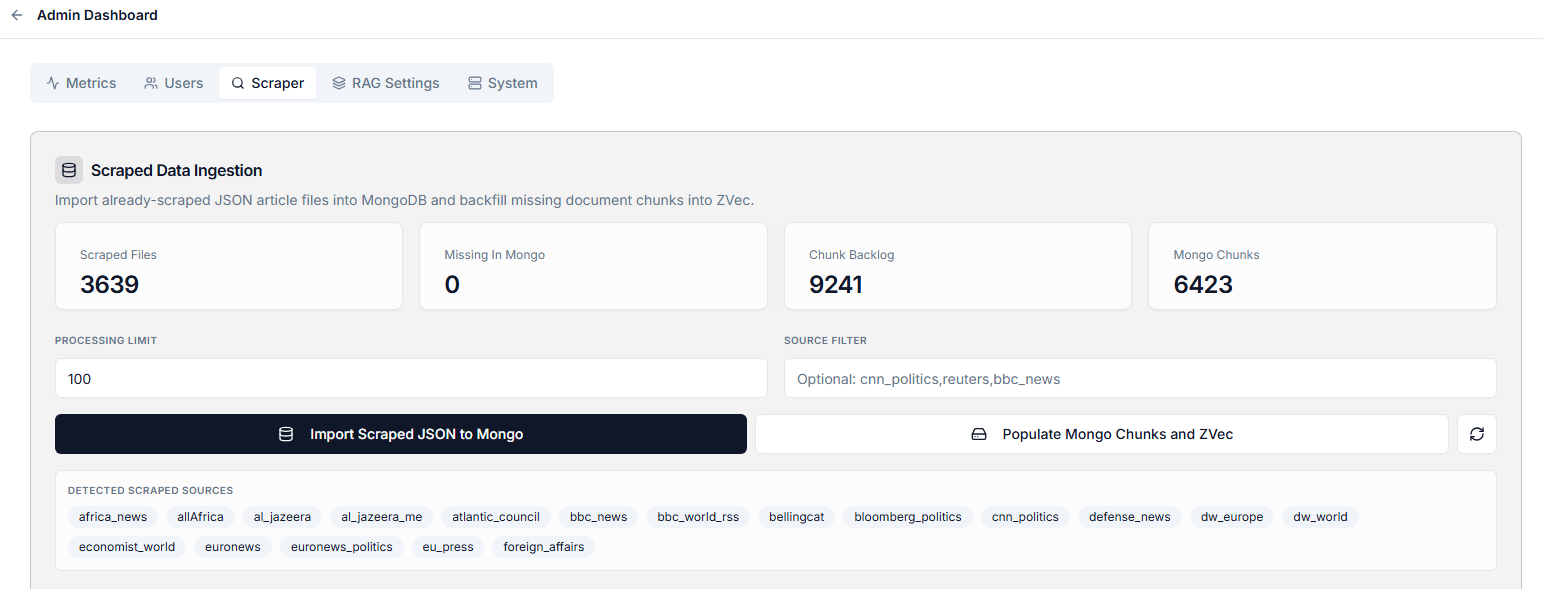
\includegraphics[width=0.96\textwidth,height=0.72\textheight,keepaspectratio]{page admin scaped data ingestion.png}
    \caption{Administration: scraped-data ingestion and vector backfill controls.}
    \label{fig:ui-admin-scraped}
\end{figure}

\begin{figure}[H]
    \centering
    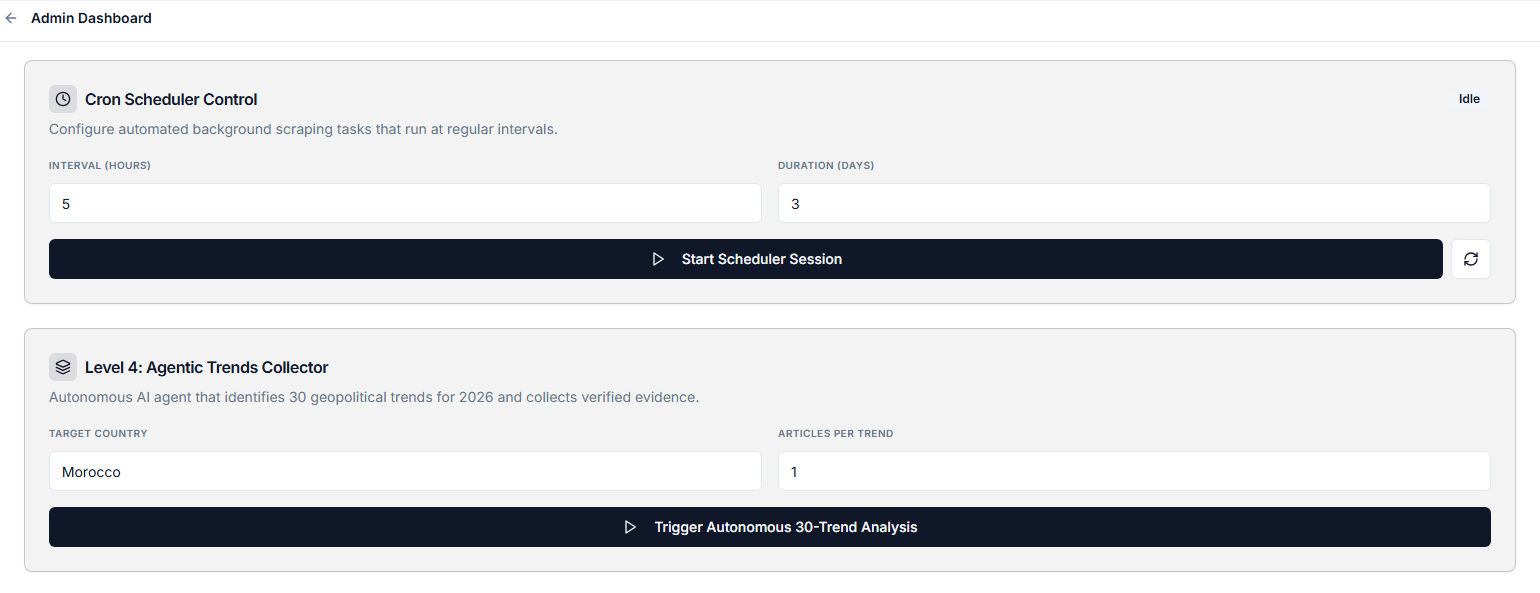
\includegraphics[width=0.96\textwidth,height=0.72\textheight,keepaspectratio]{page admin cron scheduler control and agnetic trend collector.png}
    \caption{Administration: cron scheduler and agentic trend-collection configuration.}
    \label{fig:ui-admin-cron}
\end{figure}

\begin{figure}[H]
    \centering
    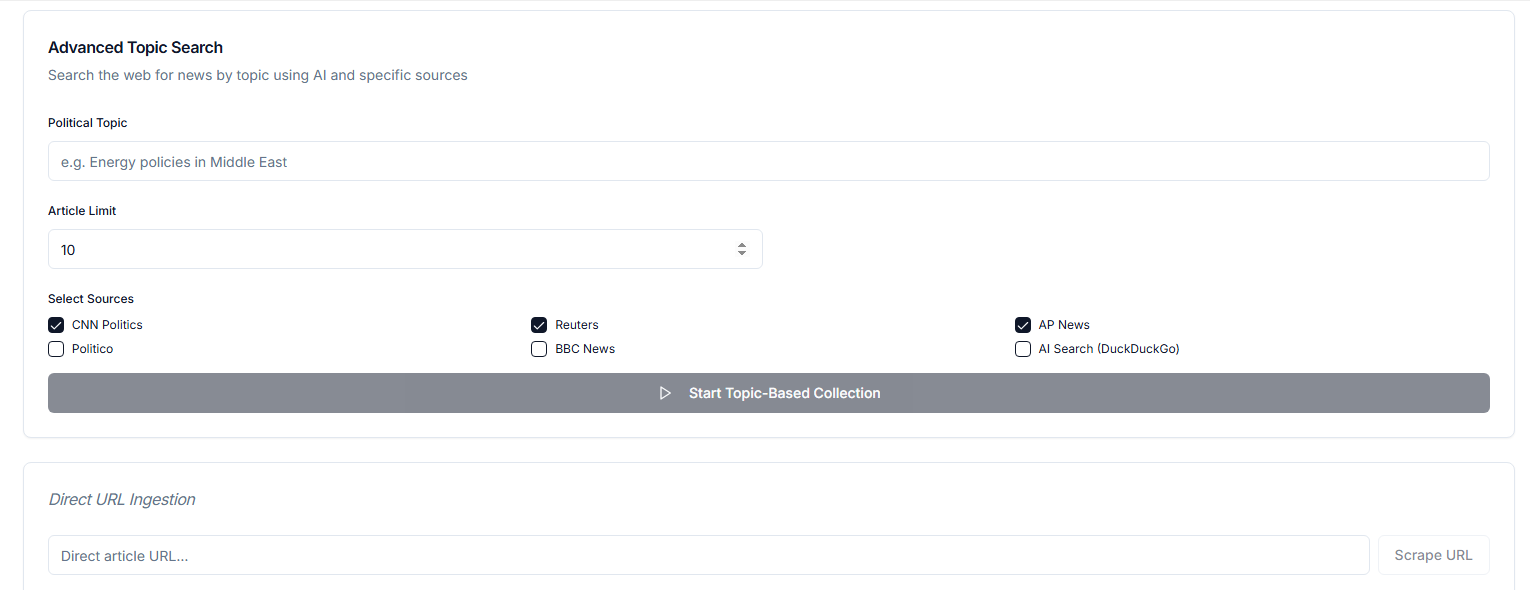
\includegraphics[width=0.96\textwidth,height=0.72\textheight,keepaspectratio]{page admin advaned topic search.png}
    \caption{Administration: advanced topic search for query-driven source discovery.}
    \label{fig:ui-admin-topic}
\end{figure}

\section{Deployment and Observability}

The stack is orchestrated with Docker Compose: MongoDB, Neo4j, Redis, FastAPI backend, React frontend (nginx), and observability services on a shared bridge network. Health checks on databases gate backend startup so the API does not accept traffic before connectors succeed. Environment variables externalize credentials and model keys, supporting reproducible deployment on sovereign infrastructure without embedding secrets in images.

OpenTelemetry instrumentation exports traces consumed by Jaeger, making multi-hop reasoning visible as a sequence of spans (API entry, retrieval, graph expansion, LLM calls, streaming response). Prometheus scrapes service metrics; Grafana dashboards track query latency, token usage, error rates, and cache behavior. Figure~\ref{fig:observability-stack} summarizes the monitoring topology; Figure~\ref{fig:deployment-topology} shows container relationships in the production compose file.

\begin{figure}[H]
    \centering
    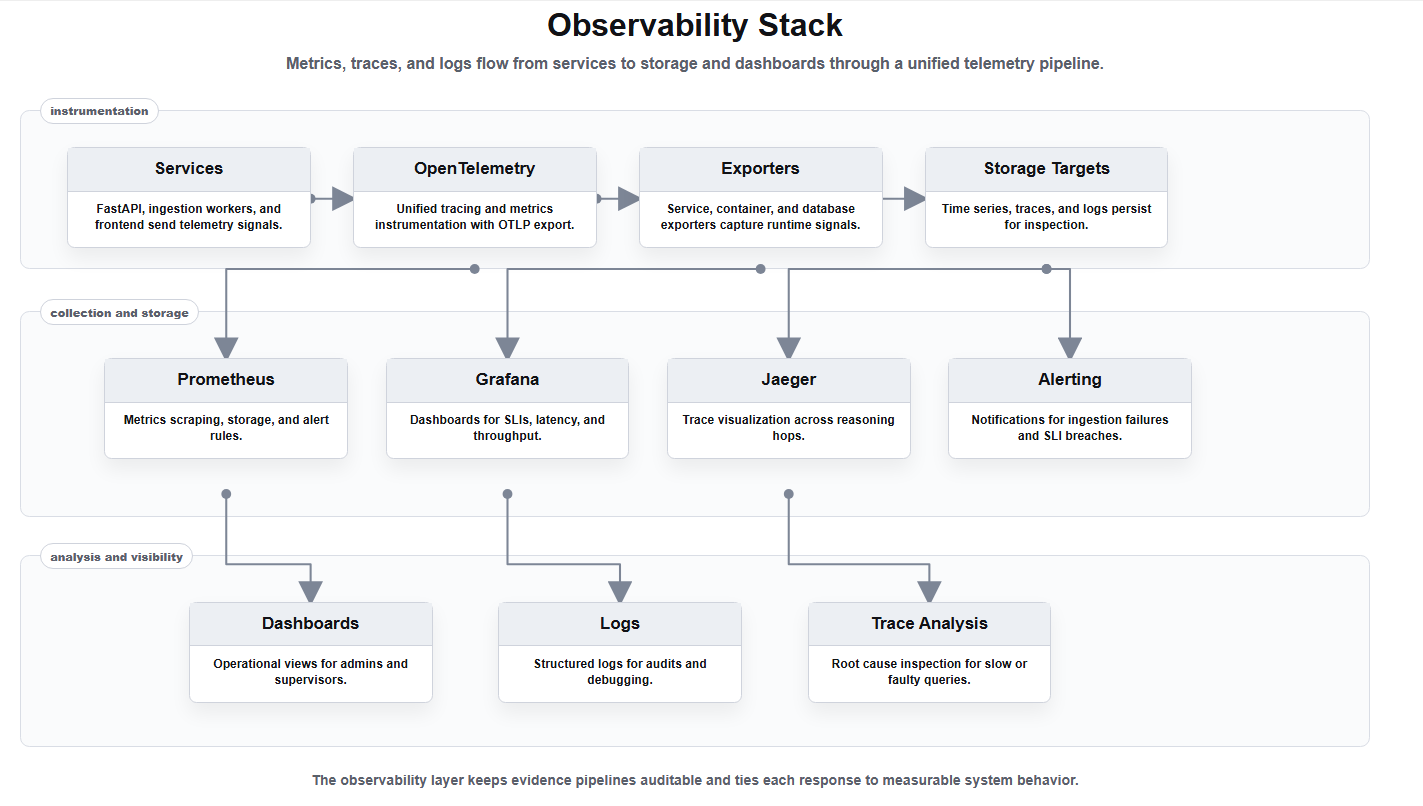
\includegraphics[width=0.96\textwidth,height=0.72\textheight,keepaspectratio]{images/observability_stack.png}
    \caption{Observability stack: metrics, dashboards, and distributed tracing.}
    \label{fig:observability-stack}
\end{figure}

\begin{figure}[H]
    \centering
    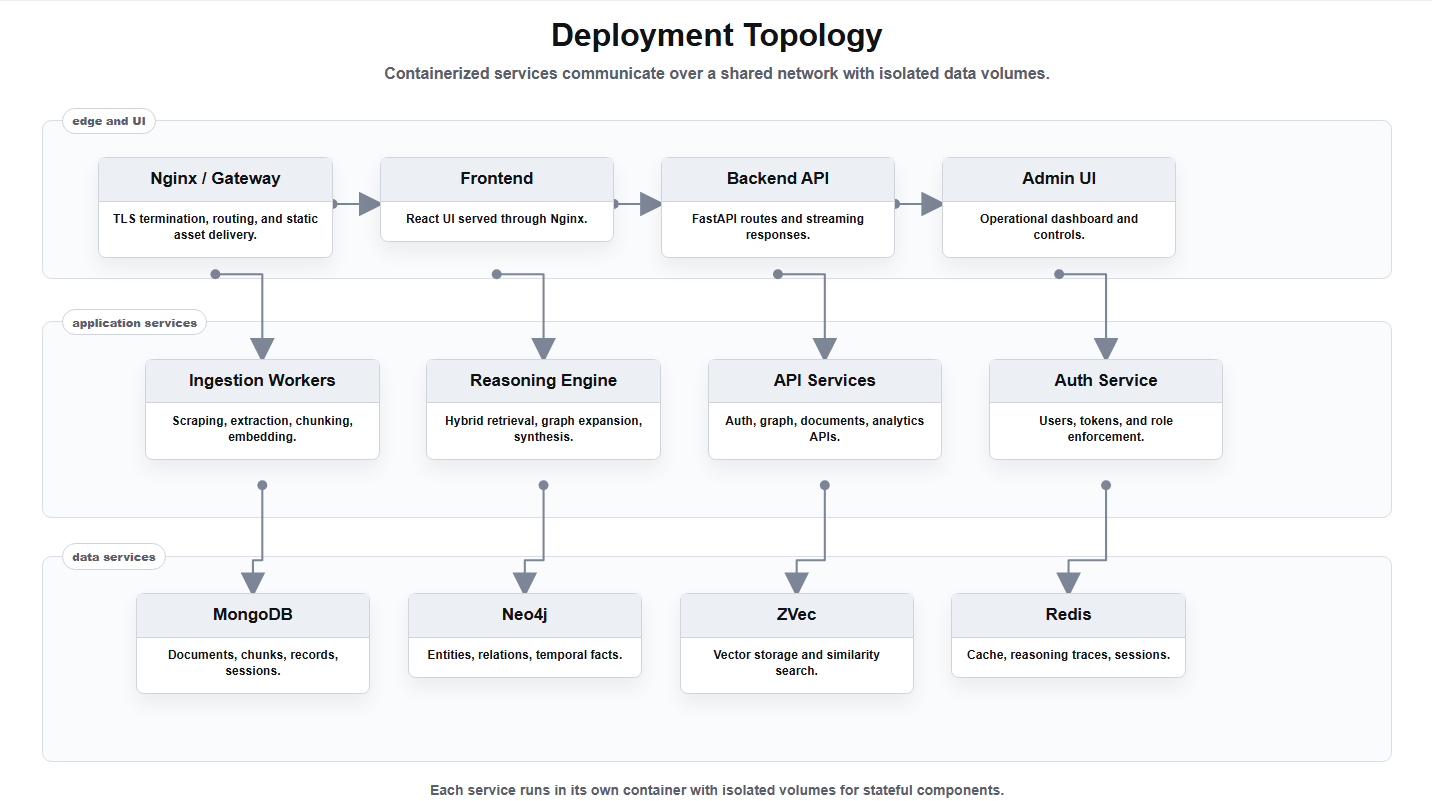
\includegraphics[width=0.96\textwidth,height=0.72\textheight,keepaspectratio]{images/deployment_topology.png}
    \caption{Deployment topology of containerized services and data stores.}
    \label{fig:deployment-topology}
\end{figure}

Resilience measures include API rate limiting with exponential backoff on external LLM calls, inter-document delays during bulk ingestion, graceful degradation when optional services are unavailable, and staged pipeline scripts (graph extract, structured extract, chunk/embed, graph publish) that can be rerun independently. The evaluation harness under \texttt{src/backend/evaluation} calls the same HTTP query endpoint as the frontend, ensuring Chapter~5 measurements reflect deployed behavior rather than isolated unit tests.

\section{Conclusion}

This chapter detailed the engineering realization of the platform: DSPy-optimized extraction, polyglot persistence with local ZVec retrieval, a three-mode reasoning engine with streaming traces, DuckDuckGo-augmented live search, a full React analytical workspace documented through operational screenshots, and a containerized observability stack. The implementation closes the gap between Chapter~3 design artifacts and runnable software. Chapter~5 will report empirical validation against the criteria defined in Chapter~2.

% Chapter 5 -- structure from table of content.md; impersonal academic style

\reportchapter{5}{Evaluation and Conclusion}{Evaluation methodology, empirical results, interpretation, contributions, limitations, and future work.}

\section{Introduction}

This chapter reports how the platform defined in Chapters~2--4 was evaluated against a curated benchmark and how the results should be interpreted. The objective is not to claim definitive superiority over all political-analysis systems, but to measure end-to-end behavior of the deployed Graph-RAG stack: retrieval from ZVec and Neo4j, synthesis with citations, and optional reasoning modes. The presentation covers the evaluation methodology, metric families, quantitative results obtained on the live backend, limitations and threats to validity, contributions of the PFE, and directions for future work.

\section{Evaluation Methodology}

Evaluation was designed to test the system as a complete platform rather than as isolated components. The harness under \texttt{src/backend/evaluation} sends each benchmark question to the same HTTP query endpoint used by the React frontend, collects the generated answer together with retrieved chunks and graph facts, and scores the output against a reference answer. This protocol ensures that reported numbers reflect deployed behavior (ingestion state, indexes, reasoning mode, and judge configuration) rather than a mocked retrieval function.

\textbf{Dataset and question categories.} The primary benchmark is stored at \texttt{benchmark/questions.jsonl} and loaded by \texttt{dataset.py}. It contains \textbf{fourteen} questions grouped into four categories aligned with political intelligence use cases: \textbf{factual} (direct entity or event lookup), \textbf{relational} (connections between actors or institutions), \textbf{temporal} (chronology and dated events), and \textbf{comparative} (synthesis across several sources or positions). Each row includes a question, a reference answer (\texttt{ground\_truth}), optional source hints, and evidence document identifiers where applicable. The mix exercises both flat retrieval and graph-dependent reasoning described in Chapter~3.

\textbf{Evaluation pipeline.} Figure~\ref{fig:state-evaluation-pipeline} summarizes the flow. Each sample is submitted to the backend in one of three reasoning modes (\texttt{rag}, \texttt{cot}, or \texttt{reflexive}). The response supplies answer text, source previews, and graph facts; the metrics module then computes RAGAS-style scores via a Mistral judge. Errors and latency are logged per sample so that failed queries do not silently skew aggregates.

\begin{figure}[H]
    \centering
    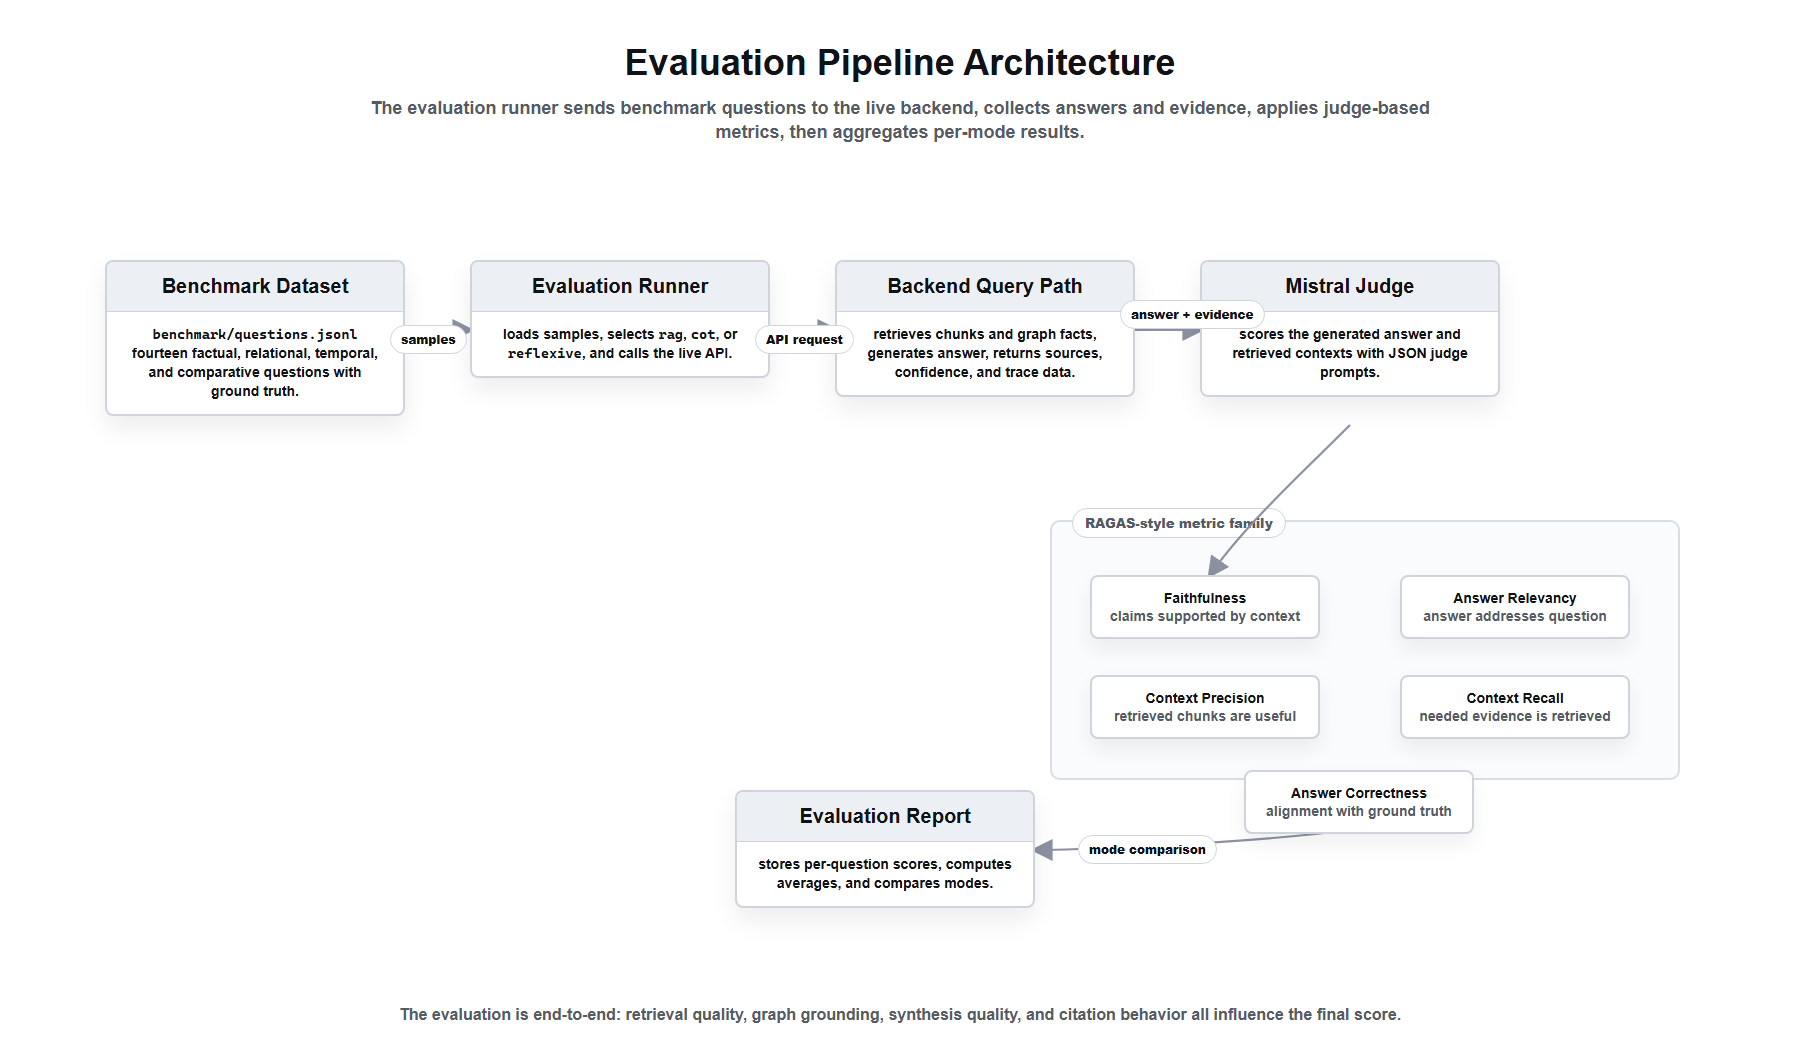
\includegraphics[width=0.96\textwidth,height=0.78\textheight,keepaspectratio]{images/state_evaluation_pipeline.png}
    \caption{Evaluation pipeline for querying the live backend and scoring generated answers.}
    \label{fig:state-evaluation-pipeline}
\end{figure}

\textbf{Experimental protocol.} The backend was invoked at \texttt{http://localhost:8001/api/v1/query} with \texttt{include\_sources=true} and \texttt{max\_hops=3}. Each of the fourteen benchmark questions was evaluated under \texttt{rag}, \texttt{cot}, and \texttt{reflexive} modes after MIPROv2 prompt optimization and corpus hardening. Each answer was judged on faithfulness, answer relevancy, context recall, and answer correctness (context precision is computed in the harness but omitted from the overview figure for readability). Aggregates are consolidated in \texttt{eval\_results.json} and per-mode files (\texttt{eval\_rag.json}, \texttt{eval\_cot.json}, \texttt{eval\_reflexive.json}); the reported run (May~2026) completed with zero backend errors on all samples.

\section{Evaluation Metrics and Results}

Three complementary metric families inform the analysis. Each answers a different quality question so that evaluation does not collapse into a single opaque score.

\textbf{Lexical metrics.} N-gram overlap compares the generated answer to the reference through contiguous word sequences, in the spirit of BLEU (precision-oriented) and ROUGE (recall-oriented) \cite{papineni-ngram,lin-rouge}. Lexical scores reward recovery of names, dates, institutions, and fixed expressions. They are strict: paraphrases that preserve meaning may score low. In political QA, lexical metrics are therefore used mainly to detect missing non-negotiable facts, not as the sole indicator of correctness.

\textbf{Semantic similarity.} Semantic Answer Similarity (SAS) measures whether two answers express the same meaning despite different surface wording \cite{risch-sas}. Embeddings and cosine similarity provide a softer signal than n-grams, which matters for relational and comparative questions where the system composes narrative answers from several evidence fragments. SAS complements lexical baselines when reference answers use alternate phrasing for the same geopolitical fact.

\textbf{RAGAS-style metrics.} The implemented harness follows the RAGAS philosophy: evaluate grounding and retrieval quality alongside the final answer \cite{ragas-paper,ragas-answer-correctness}. \textbf{Faithfulness} checks whether claims are supported by retrieved context. \textbf{Answer relevancy} measures alignment with the user question. \textbf{Context precision} and \textbf{context recall} assess whether retrieved passages contain useful and sufficient evidence. \textbf{Answer correctness} compares the generation to the ground truth through a Mistral judge (score in $[0,1]$ with short rationale). These metrics map directly to the validation criteria of Chapter~2 (grounded synthesis and inspectable evidence).

\textbf{Quantitative results.} Table~\ref{tab:mode-comparison} reports post-optimization mode-level means from \texttt{eval\_results.json} (fourteen questions, three modes, no request failures). In \texttt{rag} mode, answer correctness reaches \textbf{0.52} and answer relevancy \textbf{0.65}; faithfulness rises to \textbf{0.46} and context recall to \textbf{0.32} relative to the pre-optimization baseline. \texttt{cot} mode improves all four reported metrics (correctness \textbf{0.65}, relevancy \textbf{0.76}, faithfulness \textbf{0.58}, context recall \textbf{0.48}). \texttt{reflexive} mode achieves the strongest profile (correctness \textbf{0.80}, relevancy \textbf{0.92}, faithfulness \textbf{0.73}, context recall \textbf{0.64}), confirming that deeper reasoning and self-critique benefit political QA when retrieval supplies usable evidence.

\begin{table}[H]
\centering
\small
\setlength{\tabcolsep}{6pt}
\renewcommand{\arraystretch}{1.35}
\begin{tabularx}{\textwidth}{@{}>{\bfseries\raggedright\arraybackslash}p{2.2cm}>{\centering\arraybackslash}X>{\centering\arraybackslash}X>{\centering\arraybackslash}X>{\centering\arraybackslash}X@{}}
\toprule
\rowcolor{lightblue}
Mode & Correct. & Relev. & Faithful. & Ctx.\ recall \\
\midrule
RAG & 0.52 & 0.65 & 0.46 & 0.32 \\
CoT & 0.65 & 0.76 & 0.58 & 0.48 \\
Reflexive & 0.80 & 0.92 & 0.73 & 0.64 \\
\bottomrule
\end{tabularx}
\caption{Post-optimization RAGAS-style scores by reasoning mode (14-question benchmark, May 2026).}
\label{tab:mode-comparison}
\end{table}

Figure~\ref{fig:evaluation-results-overview} visualizes the same mode-level comparison. The monotonic gain from RAG to CoT to reflexive mode indicates that prompt optimization and reasoning depth compound; context recall remains the metric with the largest absolute lift under reflexive mode, while still leaving room for retrieval hardening.

\begin{figure}[H]
    \centering
    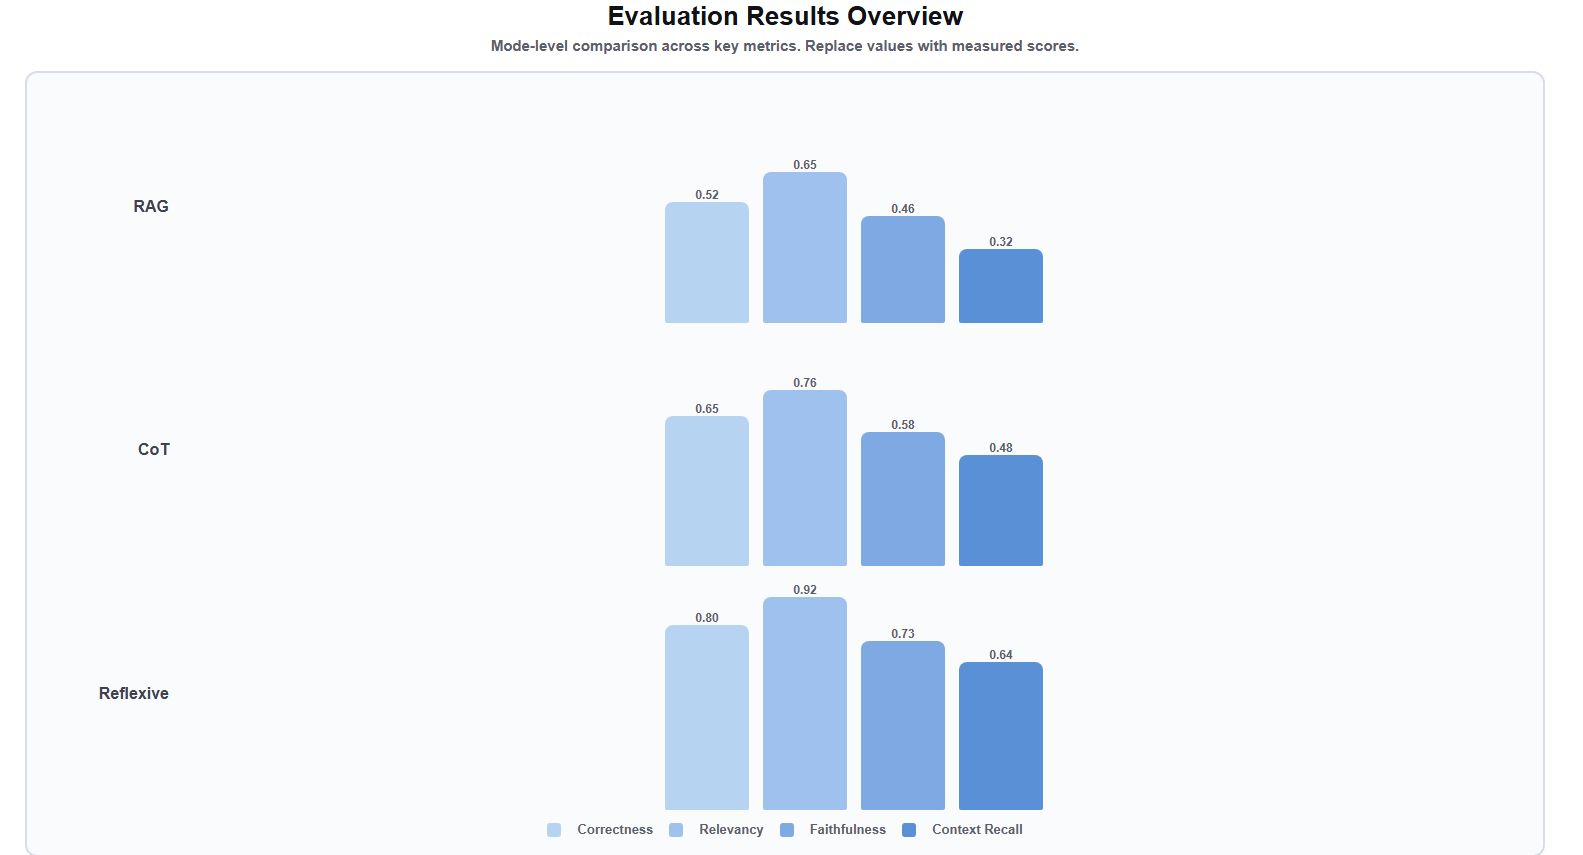
\includegraphics[width=0.92\textwidth,keepaspectratio]{images/evaluation_results_overview.png}
    \caption{Post-optimization overview of mean RAGAS-style scores by reasoning mode (correctness, relevancy, faithfulness, context recall).}
    \label{fig:evaluation-results-overview}
\end{figure}

\section{Interpretation and Limitations}

\textbf{Performance analysis.} Post-optimization scores show that the platform understands questions and grounds answers more reliably than in the first evaluation pass. \texttt{rag} mode already reaches moderate correctness and relevancy; \texttt{reflexive} mode nearly doubles context recall relative to \texttt{rag} (\textbf{0.64} vs.\ \textbf{0.32}), which supports the design choice of offering selectable reasoning depth in the UI. Remaining gaps appear on niche factual items where the corpus still lacks the exact entity or event named in the ground truth, even when the model abstains safely rather than hallucinating.

\textbf{Retrieval bottlenecks.} Context recall improves with mode complexity but remains the lowest absolute metric in \texttt{rag} mode (\textbf{0.32}). Contributing factors include corpus gaps, chunk-boundary effects, syndicated or noisy articles passing quality gates, and insufficient graph-aware reranking on the first retrieval hop. Further gains should come from ingestion expansion and reranking before additional reasoning hops, in line with validation criteria in Chapter~2.

\textbf{Threats to validity.} Four limitations bound the conclusions. \emph{Corpus coverage:} scores depend on what was ingested at evaluation time. \emph{Judge bias:} LLM-based scoring may favor fluent answers or penalize careful abstention. \emph{Temporal drift:} political facts change; the fourteen-question snapshot does not guarantee stable scores after new ingestion. \emph{Benchmark size:} the set is representative but small; enlarged benchmarks and human analyst ratings would strengthen external validity.

\section{Contributions}

The PFE delivers contributions at methodological, technical, and operational levels.

\textbf{Methodological.} A project-specific evaluation protocol combines lexical and semantic families from the literature with RAGAS-style grounding metrics executed on the live API. Question categories (factual, relational, temporal, comparative) tie metrics to analyst workflows rather than to generic QA benchmarks alone.

\textbf{Technical.} An end-to-end Graph-RAG platform integrates autonomous ingestion, ZVec semantic retrieval, Neo4j traversal, selectable reasoning modes, DuckDuckGo-augmented live search, a React analytical workspace, and containerized observability---addressing the integration gap identified in Chapter~1.

\textbf{Operational.} Staged ingestion scripts, database diagnostics, MIPROv2 prompt optimization, and the evaluation harness (\texttt{runner.py}, \texttt{compare\_modes.py}) make ingestion, retrieval, and scoring reproducible for iterative engineering.

\section{Future Work}

\textbf{Retrieval improvements.} Graph-aware reranking, stricter source filtering, query expansion, and temporal filters on edges should raise context precision and recall. Re-embedding and chunking experiments on the MongoDB corpus are the highest-impact lever given current metrics.

\textbf{Evaluation expansion.} The same fourteen-question protocol should be extended to a larger benchmark with lexical and SAS columns reported alongside RAGAS metrics, and with human analyst ratings on a stratified subset to cross-check the Mistral judge.

\textbf{Temporal modeling extensions.} Stronger validity intervals on relations, time-scoped graph queries at retrieval time, and alignment between structured legislative dates and graph edges would address weak temporal correctness scores.

\section{Conclusion}

The platform demonstrates that political Graph-RAG can be engineered as a sovereign, inspectable pipeline from ingestion to cited answers. Post-optimization evaluation on fourteen curated questions shows measurable gains across reasoning modes, with reflexive mode reaching strong relevancy and correctness while context recall remains the main lever for further improvement. The work contributes a reproducible architecture, an evaluation harness tied to production APIs, and evidence that prompt optimization and reasoning depth matter as much as raw retrieval. The bridge between unstructured political information and structured, grounded reasoning remains open for incremental hardening rather than closed as a finished product.


\begin{thebibliography}{25}
\addcontentsline{toc}{chapter}{References}

\bibitem{gdelt-official}
GDELT Project, \textit{Official GDELT website}. Available at: \url{https://www.gdeltproject.org/}.

\bibitem{gdelt-gkg}
GDELT Project, \textit{GDELT Global Knowledge Graph}. Available at: \url{https://blog.gdeltproject.org/gdelt-global-knowledge-graph/}.

\bibitem{fastapi-docs}
FastAPI, \textit{Official documentation}. Available at: \url{https://fastapi.tiangolo.com/}.

\bibitem{mongodb-docs}
MongoDB, \textit{Official documentation}. Available at: \url{https://www.mongodb.com/docs/}.

\bibitem{neo4j-docs}
Neo4j, \textit{Official documentation}. Available at: \url{https://neo4j.com/docs/}.

\bibitem{wikidata-sparql}
Wikidata, \textit{SPARQL query service}. Available at: \url{https://www.wikidata.org/wiki/Wikidata:SPARQL_query_service}.

\bibitem{celery-docs}
Celery, \textit{Official documentation}. Available at: \url{https://docs.celeryq.dev/}.

\bibitem{docker-docs}
Docker, \textit{Official documentation}. Available at: \url{https://docs.docker.com/}.

\bibitem{react-docs}
React, \textit{Official documentation}. Available at: \url{https://react.dev/}.

\bibitem{mistral-docs}
Mistral AI, \textit{Developer documentation}. Available at: \url{https://docs.mistral.ai/}.

\bibitem{lewis-rag}
P. Lewis, E. Perez, A. Piktus, F. Petroni, V. Karpukhin, N. Goyal, H. Kuttler, M. Lewis, W.-t. Yih, T. Rocktaschel, S. Riedel, and D. Kiela, \textit{Retrieval-Augmented Generation for Knowledge-Intensive NLP Tasks}, NeurIPS, 2020. Available at: \url{https://arxiv.org/abs/2005.11401}.

\bibitem{gao-rag-survey}
Y. Gao, Y. Xiong, X. Gao, K. Jia, J. Pan, Y. Bi, Y. Dai, J. Sun, and H. Wang, \textit{Retrieval-Augmented Generation for Large Language Models: A Survey}, arXiv:2312.10997, 2023. Available at: \url{https://arxiv.org/abs/2312.10997}.

\bibitem{edge-graphrag}
D. Edge, H. Trinh, N. Cheng, J. Bradley, A. Chao, A. Mody, S. Truitt, and J. Larson, \textit{From Local to Global: A Graph RAG Approach to Query-Focused Summarization}, arXiv:2404.16130, 2024. Available at: \url{https://arxiv.org/abs/2404.16130}.

\bibitem{microsoft-graphrag}
Microsoft Research, \textit{Project GraphRAG}. Available at: \url{https://www.microsoft.com/en-us/research/project/graphrag/}.

\bibitem{ragas-paper}
S. Es, J. James, L. Espinosa-Anke, and S. Schockaert, \textit{RAGAS: Automated Evaluation of Retrieval Augmented Generation}, arXiv:2309.15217, 2023. Available at: \url{https://arxiv.org/abs/2309.15217}.

\bibitem{ragas-answer-correctness}
Ragas Documentation, \textit{Answer Correctness}. Available at: \url{https://docs.ragas.io/en/v0.4.0/concepts/metrics/available_metrics/answer_correctness/}.

\bibitem{risch-sas}
J. Risch, T. Moeller, J. Gutsch, and M. Pietsch, \textit{Semantic Answer Similarity for Evaluating Question Answering Models}, arXiv:2108.06130, 2021. Available at: \url{https://arxiv.org/abs/2108.06130}.

\bibitem{lin-rouge}
C.-Y. Lin, \textit{ROUGE: A Package for Automatic Evaluation of Summaries}, Text Summarization Branches Out, Association for Computational Linguistics, 2004. Available at: \url{https://aclanthology.org/W04-1013/}.

\bibitem{papineni-ngram}
K. Papineni, \textit{Machine Translation Evaluation: N-grams to the Rescue}, LREC 2002. Available at: \url{https://research.ibm.com/publications/machine-translation-evaluation-n-grams-to-the-rescue}.

\bibitem{zvec-repo}
ZVec, \textit{ZVec GitHub Repository}. Available at: \url{https://github.com/alibaba/zvec}.

\bibitem{zvec-benchmarks}
ZVec, \textit{Benchmarks Documentation}. Available at: \url{https://zvec.org/en/docs/db/benchmarks/}.

\bibitem{proxima-engine}
Alibaba Cloud, \textit{Proxima: A Vector Retrieval Engine Independently Developed by Alibaba DAMO Academy}. Available at: \href{https://www.alibabacloud.com/blog/proxima-a-vector-retrieval-engine-independently-developed-by-alibaba-damo-academy_597250}{Alibaba Cloud technical blog}.

\bibitem{faiss-docs}
Meta AI Research, \textit{FAISS Documentation}. Available at: \url{https://faiss.ai/}.

\bibitem{qdrant-docs}
Qdrant, \textit{Qdrant Documentation}. Available at: \url{https://qdrant.tech/documentation/}.

\bibitem{weaviate-docs}
Weaviate, \textit{Weaviate Documentation}. Available at: \url{https://docs.weaviate.io/weaviate}.

\bibitem{milvus-docs}
Milvus, \textit{Milvus Documentation}. Available at: \url{https://milvus.io/docs/}.

\bibitem{chroma-docs}
Chroma, \textit{Chroma Documentation}. Available at: \url{https://docs.trychroma.com/}.

\bibitem{elasticsearch-vector-docs}
Elastic, \textit{Vector Search Documentation}. Available at: \url{https://www.elastic.co/docs/solutions/search/vector}.

\bibitem{opensearch-vector-docs}
OpenSearch, \textit{Vector Search Documentation}. Available at: \url{https://docs.opensearch.org/latest/vector-search/}.

\bibitem{langchain-splitters}
LangChain, \textit{Text Splitters Documentation}. Available at: \url{https://docs.langchain.com/oss/python/integrations/splitters}.

\bibitem{llamaindex-node-parsers}
LlamaIndex, \textit{Node Parser Modules}. Available at: \url{https://developers.llamaindex.ai/python/framework/module_guides/loading/node_parsers/}.

\bibitem{vaswani-attention}
A. Vaswani, N. Shazeer, N. Parmar, J. Uszkoreit, L. Jones, A. N. Gomez, L. Kaiser, and I. Polosukhin, \textit{Attention Is All You Need}, NeurIPS, 2017. Available at: \url{https://arxiv.org/abs/1706.03762}.

\bibitem{gfg-llm-architecture}
GeeksforGeeks, \textit{LLM Architecture}, updated October 28, 2025. Available at: \href{https://www.geeksforgeeks.org/artificial-intelligence/exploring-the-technical-architecture-behind-large-language-models/}{GeeksforGeeks: LLM Architecture}.

\bibitem{wei-cot}
J. Wei, X. Wang, D. Schuurmans, M. Bosma, B. Ichter, F. Xia, E. Chi, Q. V. Le, and D. Zhou, \textit{Chain-of-Thought Prompting Elicits Reasoning in Large Language Models}, NeurIPS, 2022. Available at: \url{https://arxiv.org/abs/2201.11903}.

\bibitem{khattab-dspy}
O. Khattab, C. Singh, D. Zhang, Y. Dann, L. Li, E. Ma, and C. Potts, \textit{DSPy: Compiling Declarative Language Model Calls into Self-Improving Pipelines}, ICLR, 2024. Available at: \url{https://arxiv.org/abs/2310.03714}.

\bibitem{allaway-stance}
E. Allaway and K. McKeown, \textit{Zero-shot Stance Detection: A Dataset and Model using Generalized Topic Representations}, EMNLP, 2020. Available at: \url{https://aclanthology.org/2020.emnlp-main.673/}.

\bibitem{trivedi-hyte}
S. Trivedi, H. Wang, and J. Tang, \textit{HyTE: Hyperplane-based Temporally aware Entity Embedding}, WWW, 2018. Available at: \url{https://doi.org/10.1145/3178876.3186048}.

\bibitem{yao-react}
S. Yao, J. Zhao, D. Yu, N. Du, I. Shafran, K. Narasimhan, and Y. Cao, \textit{ReAct: Synergizing Reasoning and Acting in Language Models}, ICLR, 2023. Available at: \url{https://arxiv.org/abs/2210.03629}.

\bibitem{trivedi-ircot}
H. Trivedi, N. Balasubramanian, T. Khot, and A. Sabharwal, \textit{Interleaving Retrieval with Chain-of-Thought Reasoning for Knowledge-Intensive Multi-Hop Questions}, ACL, 2023. Available at: \url{https://aclanthology.org/2023.acl-long.135/}.

\bibitem{asai-selfrag}
Y. Asai, C. Wu, J. Wang, W. Sil, and H. Hajishirzi, \textit{Self-RAG: Learning to Retrieve, Generate, and Critique through Self-Reflection}, ICLR, 2024. Available at: \url{https://arxiv.org/abs/2310.11511}.

\end{thebibliography}


\end{document}